\documentclass[11pt,a4paper,dvipsnames,twosided]{article}
\usepackage[deliverable]{IOHKCoverPage}

% data for Deliverable header -- added by KH from an EU H2020 project template
\DeliverableNumber{SL-D5}
\DeliverableTitle{A Formal Specification of the Cardano Ledger}{Formal Cardano Ledger Spec.}
\DeliverableResponsible{Formal Methods Team}
\EditorName{Jared Corduan, \IOHK}
\Authors{Jared Corduan \quad \texttt{<jared.corduan@iohk.io>}
   \\[1em]
   Polina Vinogradova \quad \texttt{<polina.vinogradova@iohk.io>}
   \\[1em]
   Matthias G\"udemann \quad \texttt{<matthias.gudemann@iohk.io>}
}
\DueDate{15$^{\textrm{th}}$ October 2019}
\SubmissionDate{8th October 2019}{2019/10/08}
\LeaderName{Philipp Kant, \IOHK}
\InstitutionAddress{\IOHK}
\Version{1.0}
\Project{Shelley Ledger}
\DisseminationPU

\usepackage[margin=2.5cm]{geometry}
\usepackage{lscape}
\usepackage{iohk}
\usepackage{microtype}
\usepackage{mathpazo} % nice fonts
\usepackage{amsmath}
\usepackage{amssymb}
\usepackage{amsthm}
\usepackage{latexsym}
\usepackage{mathtools}
\usepackage{stmaryrd}
\usepackage{extarrows}
\usepackage{slashed}
\usepackage[unicode=true,pdftex,pdfa,colorlinks=true]{hyperref}
\usepackage{xcolor}
\usepackage[capitalise,noabbrev,nameinlink]{cleveref}
\usepackage{float}
\floatstyle{boxed}
\restylefloat{figure}
\usepackage{tikz}
\usepackage{booktabs}
\usepackage{enumerate}
\usepackage{listings}
%%
%% Package `semantic` can be used for writing inference rules.
%%
\usepackage{semantic}
%% Setup for the semantic package
\setpremisesspace{20pt}

\usepackage{tocloft}
\addtolength{\cftsubsecnumwidth}{5pt}

%%
%% Types
%%
\newcommand{\Nothing}{\ensuremath{\Diamond}}
\newcommand{\N}{\ensuremath{\mathbb{N}}}
\newcommand{\Bool}{\type{Bool}}
\newcommand{\Npos}{\ensuremath{\mathbb{N}^{>0}}}
\newcommand{\Z}{\ensuremath{\mathbb{Z}}}
\newcommand{\Q}{\ensuremath{\mathbb{Q}}}
\newcommand{\R}{\ensuremath{\mathbb{R}}}
\newcommand{\Rnn}{\ensuremath{\mathbb{R}^{\geq 0}}}
\newcommand{\Tx}{\type{Tx}}
\newcommand{\TxBody}{\type{TxBody}}
\newcommand{\TxWitness}{\type{TxWitness}}
\newcommand{\Ix}{\type{Ix}}
\newcommand{\TxId}{\type{TxId}}
\newcommand{\Addr}{\type{Addr}}
\newcommand{\UTxO}{\type{UTxO}}
\newcommand{\Wdrl}{\type{Wdrl}}
\newcommand{\Coin}{\type{Coin}}
\newcommand{\PParams}{\type{PParams}}
\newcommand{\PParamsUpdate}{\type{PParamsUpdate}}
\newcommand{\ProposedPPUpdates}{\type{ProposedPPUpdates}}
\newcommand{\Slot}{\type{Slot}}
\newcommand{\StabilityWindow}{\ensuremath{\mathsf{StabilityWindow}}}
\newcommand{\RandomnessStabilisationWindow}{\ensuremath{\mathsf{RandomnessStabilisationWindow}}}
\newcommand{\SlotsPerEpoch}{\mathsf{SlotsPerEpoch}}
\newcommand{\SlotsPerKESPeriod}{\mathsf{SlotsPerKESPeriod}}
\newcommand{\MaxMajorPV}{\mathsf{MaxMajorPV}}
\newcommand{\ActiveSlotCoeff}{\mathsf{ActiveSlotCoeff}}
\newcommand{\Network}{\mathsf{Network}}
\newcommand{\NetworkId}{\mathsf{NetworkId}}
\newcommand{\BlockNo}{\type{BlockNo}}
\newcommand{\MaxKESEvo}{\ensuremath{\mathsf{MaxKESEvo}}}
\newcommand{\Quorum}{\ensuremath{\mathsf{Quorum}}}
\newcommand{\MaxLovelaceSupply}{\ensuremath{\mathsf{MaxLovelaceSupply}}}
\newcommand{\Duration}{\type{Duration}}
\newcommand{\StakePools}{\type{StakePools}}
\newcommand{\Seed}{\type{Seed}}
\newcommand{\seedOp}{\star}
\newcommand{\Ppm}{\type{Ppm}}
\newcommand{\ProtVer}{\ensuremath{\type{ProtVer}}}
\newcommand{\Metadatum}{\ensuremath{\type{Metadatum}}}
\newcommand{\Metadata}{\ensuremath{\type{Metadata}}}
\newcommand{\MetadataHash}{\ensuremath{\type{MetadataHash}}}
\newcommand{\Update}{\type{Update}}
\newcommand{\GenesisDelegation}{\type{GenesisDelegation}}
\newcommand{\FutGenesisDelegation}{\type{FutGenesisDelegation}}

\newcommand{\DCert}{\type{DCert}}
\newcommand{\DCertRegKey}{\type{DCert_{regkey}}}
\newcommand{\DCertDeRegKey}{\type{DCert_{deregkey}}}
\newcommand{\DCertDeleg}{\type{DCert_{delegate}}}
\newcommand{\DCertRegPool}{\type{DCert_{regpool}}}
\newcommand{\DCertRetirePool}{\type{DCert_{retirepool}}}
\newcommand{\DCertGen}{\type{DCert_{genesis}}}
\newcommand{\DCertMir}{\type{DCert_{mir}}}
\newcommand{\PoolParam}{\type{PoolParam}}
\newcommand{\PoolMD}{\type{PoolMD}}
\newcommand{\MIRPot}{\type{MIRPot}}
\newcommand{\InstantaneousRewards}{\type{InstantaneousRewards}}
\newcommand{\ReservesMIR}{\type{ReservesMIR}}
\newcommand{\TreasuryMIR}{\type{TreasuryMIR}}
\newcommand{\URL}{\type{Url}}
\newcommand{\UTxOState}{\ensuremath{\type{UTxOState}}}
\newcommand{\ledgerState}{\ensuremath{\type{ledgerState}}}

\newcommand{\AddrRWD}{\type{Addr_{rwd}}}
\newcommand{\AddrB}{\type{Addr_{base}}}
\newcommand{\AddrP}{\type{Addr_{ptr}}}
\newcommand{\AddrE}{\type{Addr_{enterprise}}}
\newcommand{\AddrBS}{\type{Addr_{bootstrap}}}
\newcommand{\Ptr}{\type{Ptr}}
\newcommand{\DState}{\type{DState}}
\newcommand{\DWEnv}{\type{DWEnv}}
\newcommand{\DPSEnv}{\type{DPSEnv}}
\newcommand{\DPEnv}{\type{DPEnv}}
\newcommand{\DEnv}{\type{DEnv}}
\newcommand{\PEnv}{\type{PEnv}}
\newcommand{\DPState}{\type{DPState}}
\newcommand{\PState}{\type{PState}}
\newcommand{\DCertBody}{\type{DCertBody}}
\newcommand{\TData}{\type{TData}}
\newcommand{\DPoolReap}{\ensuremath{\type{poolreap}}}
\newcommand{\UPIState}{\type{UPIState}}
\newcommand{\UpdatePayload}{\type{UpdatePayload}}

% multi-signature
\newcommand{\StakeCredential}{\type{Credential}_{stake}}

\newcommand{\txwitsVKey}[1]{\fun{txwitsVKey}~\var{#1}}
\newcommand{\txwitsScript}[1]{\fun{txwitsScript}~\var{#1}}

\newcommand{\AddrVKey}{\type{Addr^{vkey}}}
\newcommand{\AddrRWDVKey}{\type{Addr_{rwd}^{vkey}}}
\newcommand{\AddrRWDScr}{\type{Addr_{rwd}^{script}}}
\newcommand{\AddrVKeyB}{\type{Addr^{vkey}_{base}}}
\newcommand{\AddrVKeyP}{\type{Addr^{vkey}_{ptr}}}
\newcommand{\AddrVKeyE}{\type{Addr^{vkey}_{enterprise}}}
\newcommand{\AddrVKeyBS}{\type{Addr^{vkey}_{bootstrap}}}
\newcommand{\AddrScr}{\type{Addr^{script}}}
\newcommand{\AddrScrBase}{\type{Addr_{base}^{script}}}
\newcommand{\AddrScrEnterprise}{\type{Addr_{enterprise}^{script}}}
\newcommand{\AddrScrPtr}{\type{Addr_{ptr}^{script}}}
\newcommand{\HashScr}{\type{ScriptHash}}
\newcommand{\Script}{\type{Script}}
\newcommand{\MSig}{\type{MSig}}
\newcommand{\Credential}{\type{Credential}}

%% Adding witnesses
\newcommand{\TxIn}{\type{TxIn}}
\newcommand{\TxOut}{\type{TxOut}}
\newcommand{\VKey}{\type{VKey}}
\newcommand{\VKeyEv}{\type{VKey_{ev}}}
\newcommand{\VKeyGen}{\type{VKey_G}}
\newcommand{\SKey}{\type{SKey}}
\newcommand{\SKeyEv}{\type{SKey_{ev}}}
\newcommand{\KeyHash}{\type{KeyHash}}
\newcommand{\KeyHashGen}{\type{KeyHash_G}}
\newcommand{\KeyPair}{\type{KeyPair}}
\newcommand{\KeyPairEv}{\type{KeyPair_{ev}}}
\newcommand{\Sig}{\type{Sig}}
\newcommand{\Data}{\type{Data}}
\newcommand{\Ser}{\type{Ser}}
%% Adding delegation
\newcommand{\Epoch}{\type{Epoch}}
\newcommand{\KESPeriod}{\type{KESPeriod}}
%% Blockchain
\newcommand{\Acnt}{\type{Acnt}}
\newcommand{\Gkeys}{\var{G_{keys}}}
\newcommand{\Block}{\type{Block}}
\newcommand{\SlotId}{\type{SlotId}}
\newcommand{\PPUpdateState}{\type{PPUpdateState}}
\newcommand{\PPUpdateEnv}{\type{PPUpdateEnv}}
\newcommand{\UTxOEnv}{\type{UTxOEnv}}
\newcommand{\CEEnv}{\type{CEEnv}}
\newcommand{\CEState}{\type{CEState}}
\newcommand{\BDEnv}{\type{BDEnv}}
\newcommand{\BDState}{\type{BDState}}
\newcommand{\LEnv}{\type{LEnv}}
\newcommand{\LState}{\type{LState}}

\newcommand{\Proof}{\type{Proof}}
\newcommand{\Seedl}{\mathsf{Seed}_\ell}
\newcommand{\Seede}{\mathsf{Seed}_\eta}
\newcommand{\slotToSeed}[1]{\fun{slotToSeed}~ \var{#1}}
\newcommand{\prevHashToNonce}[1]{\fun{prevHashToNonce}~ \var{#1}}
\newcommand{\isOverlaySlot}[3]{\fun{isOverlaySlot}~\var{#1}~\var{#2}~\var{#3}}
\newcommand{\classifyOverlaySlot}[5]{\fun{classifyOverlaySlot}~\var{#1}~\var{#2}~\var{#3}~\var{#4}~\var{#5}}

\newcommand{\T}{\type{T}}
\newcommand{\vrf}[3]{\fun{vrf}_{#1} ~ #2 ~ #3}
\newcommand{\verifyVrf}[4]{\fun{verifyVrf}_{#1} ~ #2 ~ #3 ~#4}

\newcommand{\HashHeader}{\type{HashHeader}}
\newcommand{\HashBBody}{\type{HashBBody}}
\newcommand{\bhHash}[1]{\fun{bhHash}~ \var{#1}}
\newcommand{\bHeaderSize}[1]{\fun{bHeaderSize}~ \var{#1}}
\newcommand{\bSize}[1]{\fun{bSize}~ \var{#1}}
\newcommand{\bBodySize}[1]{\fun{bBodySize}~ \var{#1}}
\newcommand{\OCert}{\type{OCert}}
\newcommand{\BHeader}{\type{BHeader}}
\newcommand{\BHBody}{\type{BHBody}}

\newcommand{\bheader}[1]{\fun{bheader}~\var{#1}}
\newcommand{\hsig}[1]{\fun{hsig}~\var{#1}}
\newcommand{\bprev}[1]{\fun{bprev}~\var{#1}}
\newcommand{\bhash}[1]{\fun{bhash}~\var{#1}}
\newcommand{\bvkcold}[1]{\fun{bvkcold}~\var{#1}}
\newcommand{\bseedl}[1]{\fun{bseed}_{\ell}~\var{#1}}
\newcommand{\bprfn}[1]{\fun{bprf}_{n}~\var{#1}}
\newcommand{\bseedn}[1]{\fun{bseed}_{n}~\var{#1}}
\newcommand{\bprfl}[1]{\fun{bprf}_{\ell}~\var{#1}}
\newcommand{\bocert}[1]{\fun{bocert}~\var{#1}}
\newcommand{\bnonce}[1]{\fun{bnonce}~\var{#1}}
\newcommand{\bleader}[1]{\fun{bleader}~\var{#1}}
\newcommand{\hBbsize}[1]{\fun{hBbsize}~\var{#1}}
\newcommand{\bbodyhash}[1]{\fun{bbodyhash}~\var{#1}}
\newcommand{\overlaySchedule}[3]{\fun{overlaySchedule}~\var{#1}~\var{#2}~\var{#3}}

\newcommand{\OCertEnv}{\type{OCertEnv}}
\newcommand{\PrtclState}{\type{PrtclState}}
\newcommand{\PrtclEnv}{\type{PrtclEnv}}
\newcommand{\OverlayEnv}{\type{OverlayEnv}}
\newcommand{\VRFState}{\type{VRFState}}
\newcommand{\TickNonceState}{\type{TickNonceState}}
\newcommand{\TickNonceEnv}{\type{TickNonceEnv}}
\newcommand{\NewEpochState}{\type{NewEpochState}}
\newcommand{\UpdateNonceState}{\type{UpdateNonceState}}
\newcommand{\UpdateNonceEnv}{\type{UpdateNonceEnv}}
\newcommand{\PoolDistr}{\type{PoolDistr}}
\newcommand{\BBodyEnv}{\type{BBodyEnv}}
\newcommand{\BBodyState}{\type{BBodyState}}
\newcommand{\RUpdEnv}{\type{RUpdEnv}}
\newcommand{\ChainEnv}{\type{ChainEnv}}
\newcommand{\ChainState}{\type{ChainState}}
\newcommand{\ChainSig}{\type{ChainSig}}
\newcommand{\LastAppliedBlock}{\type{LastAppliedBlock}}
\newcommand{\lastAppliedHash}[1]{\fun{lastAppliedHash}~\var{#1}}


%%
%% Functions
%%
\newcommand{\txins}[1]{\fun{txins}~ \var{#1}}
\newcommand{\txouts}[1]{\fun{txouts}~ \var{#1}}
\newcommand{\txcerts}[1]{\fun{txcerts}~ \var{#1}}
\newcommand{\txid}[1]{\fun{txid}~ \var{#1}}
\newcommand{\outs}[1]{\fun{outs}~ \var{#1}}
\newcommand{\values}[1]{\fun{values}~ #1}
\newcommand{\ubalance}[1]{\fun{ubalance}~ \var{#1}}
\newcommand{\txttl}[1]{\fun{txttl}~ \var{#1}}
\newcommand{\firstSlot}[1]{\fun{firstSlot}~ \var{#1}}
\newcommand{\totalDeposits}[3]{\fun{totalDeposits}~ \var{#1} ~ \var{#2} ~ \var{#3}}
\newcommand{\keyRefund}[6]{\fun{keyRefund}~ {#1}~{#2}~{#3}~\var{#4}~\var{#5}~\var{#6}}
\newcommand{\refund}[4]{\fun{refund}~ \var{#1}~ \var{#2}~ {#3}~ {#4}}
\newcommand{\keyRefunds}[2]{\fun{keyRefunds}~ \var{#1}~ \var{#2}}
\newcommand{\consumed}[2]{\fun{consumed}~ \var{#1}~ \var{#2}}
\newcommand{\produced}[2]{\fun{produced}~ \var{#1}~ \var{#2}}
\newcommand{\applyFun}[2]{\fun{#1}~\var{#2}}

\newcommand{\RegKey}[1]{\textsc{RegKey}(#1)}
\newcommand{\DeregKey}[1]{\textsc{DeregKey}(#1)}
\newcommand{\Delegate}[1]{\textsc{Delegate}(#1)}
\newcommand{\RegPool}[1]{\textsc{RegPool}(#1)}
\newcommand{\RetirePool}[1]{\textsc{RetirePool}(#1)}
\newcommand{\cwitness}[1]{\fun{cwitness}~ \var{#1}}
\newcommand{\dpool}[1]{\fun{dpool}~ \var{#1}}
\newcommand{\poolParam}[1]{\fun{poolParam}~ \var{#1}}
\newcommand{\retire}[1]{\fun{retire}~ \var{#1}}
\newcommand{\addrRw}[1]{\fun{addr_{rwd}}~ \var{#1}}
\newcommand{\epoch}[1]{\fun{epoch}~\var{#1}}
\newcommand{\kesPeriod}[1]{\fun{kesPeriod}~\var{#1}}

%% UTxO witnesses
\newcommand{\inputs}[1]{\fun{inputs}~ \var{#1}}
\newcommand{\txwits}[1]{\fun{txwits}~ \var{#1}}
\newcommand{\verify}[3]{\fun{verify} ~ #1 ~ #2 ~ #3}
\newcommand{\sign}[2]{\fun{sign} ~ #1 ~ #2}
\newcommand{\verifyEv}[4]{\fun{verify_{ev}} ~ #1 ~ #2 ~ #3 ~ #4}
\newcommand{\signEv}[3]{\fun{sign_{ev}} ~ #1 ~ #2 ~ #3}
\newcommand{\serialised}[1]{\llbracket \var{#1} \rrbracket}
\newcommand{\hashKey}[1]{\fun{hashKey}~ \var{#1}}
\newcommand{\txbody}[1]{\fun{txbody}~ \var{#1}}
\newcommand{\txfee}[1]{\fun{txfee}~ \var{#1}}
\newcommand{\txwdrls}[1]{\fun{txwdrls}~ \var{#1}}
\newcommand{\minfee}[2]{\fun{minfee}~ \var{#1}~ \var{#2}}
\newcommand{\slotminus}[2]{\var{#1}~-_{s}~\var{#2}}
\DeclarePairedDelimiter\floor{\lfloor}{\rfloor}
% wildcard parameter
\newcommand{\wcard}[0]{\rule[-.5mm]{2mm}{.2mm}}
%% Adding ledgers...
\newcommand{\utxo}[1]{\fun{utxo}~ #1}
%% Delegation
\newcommand{\delegatesName}{\fun{delegates}}
\newcommand{\delegates}[3]{\delegatesName~#1~#2~#3}
\newcommand{\dwho}[1]{\fun{dwho}~\var{#1}}
\newcommand{\depoch}[1]{\fun{depoch}~\var{#1}}
\newcommand{\dval}{\ensuremath{d_{\mathsf{val}}}}
%% Delegation witnesses
\newcommand{\dbody}[1]{\fun{dbody}~\var{#1}}
\newcommand{\dwit}[1]{\fun{dwit}~\var{#1}}
%% Blockchain
\newcommand{\bwit}[1]{\fun{bwit}~\var{#1}}
\newcommand{\bslot}[1]{\fun{bslot}~\var{#1}}
\newcommand{\bblockno}[1]{\fun{bblockno}~\var{#1}}
\newcommand{\bbody}[1]{\fun{bbody}~\var{#1}}
\newcommand{\bhbody}[1]{\fun{bhbody}~\var{#1}}
\newcommand{\bdlgs}[1]{\fun{bdlgs}~\var{#1}}
%% ledgerstate constants
\newcommand{\genesisId}{\ensuremath{Genesis_{Id}}}
\newcommand{\genesisTxOut}{\ensuremath{Genesis_{Out}}}
\newcommand{\genesisUTxO}{\ensuremath{Genesis_{UTxO}}}
\newcommand{\genesisUTxOState}{(\genesisUTxO,\wcard,\wcard,\wcard)}
\newcommand{\emax}{\ensuremath{\mathsf{E_{max}}}}

\newcommand{\unitInterval}{\ensuremath{[0,~1]}}
\newcommand{\unitIntervalNonNull}{\ensuremath{(0,~1]}}
\newcommand{\nonnegReals}{\ensuremath{[0,~\infty)}}
\newcommand{\posReals}{\ensuremath{(0,~\infty)}}

\theoremstyle{definition}
\newtheorem{definition}{Definition}[section]
\newtheorem{lemma}[definition]{Lemma}
\newtheorem{theorem}[definition]{Theorem}
\newtheorem{property}{Property}[section]

\newcommand{\leteq}{\ensuremath{\mathrel{\mathop:}=}}

\begin{document}

\hypersetup{
  pdftitle={A Formal Specification of the Cardano Ledger (Byron Release)},
  breaklinks=true,
  bookmarks=true,
  colorlinks=false,
  linkcolor={blue},
  citecolor={blue},
  urlcolor={blue},
  linkbordercolor={white},
  citebordercolor={white},
  urlbordercolor={white}
}

\title{
  A Formal Specification of the Cardano Ledger\\
  \small{(for the Byron release)}
}

\author{Damian Nadales \\
  {\small \texttt{damian.nadales@iohk.io}}\\
}

\date{\today}

\maketitle

\begin{abstract}
  This document defines the rules for extending a ledger with transactions, as
  implemented in the Byron release of the Cardano Ledger. It is intended to
  serve as the specification for random generators of transactions which adhere
  to the rules presented here.
\end{abstract}

\section*{List of Contributors}
\label{acknowledgements}

Jared Corduan, Nicholas Clarke, Marko Dimjašević, Duncan Coutts, Ru Horlick,
Michael Hueschen, Ryan Lemmer.


\section{Introduction}
\label{sec:introduction}

This specification models the \textit{conditions} that the different parts of a
transaction have to fulfill so that they can extend a ledger, which is
represented here as a list of transactions. In particular, we model the
following aspects:

\begin{description}
\item[Preservation of value] relationship between the total value of input and
  outputs in a new transaction, and the unspent outputs.
\item[Witnesses] authentication of parts of the transaction data by means of
  cryptographic entities (such as signatures and private keys) contained in
  these transactions.
\item[Delegation] validity of delegation certificates, which delegate
  block-signing rights.
\item[Update validation] voting mechanism which captures the identification of
  the voters, and the participants that can post update proposals.
\end{description}

The following aspects will not be modeled (since they are not part of the Byron
release):
\begin{description}
\item[Stake] staking rights associated to an addresses.
\end{description}

\section{Notation}\label{sec:notation}

\begin{description}
\item[Natural Numbers] The set $\mathbb{N}$ refers to the set of all natural
  numbers $\{0, 1, 2, \ldots\}$. The set $\mathbb{Q}$ refers to the set of
  rational numbers.
\item[Booleans] The set $\mathbb{B}$ denotes the set of booleans
  $\{\var{True}, \var{False}\}$.
\item[Powerset] Given a set $\type{X}$, $\powerset{\type{X}}$ is the set of all
  the subsets of $X$.
\item[Sequences] Given a set $\type{X}$, $\seqof{\type{X}}$ is the set of
  sequences having elements taken from $\type{X}$. The empty sequence is
  denoted by $\epsilon$, and given a sequence $\Lambda$, $\Lambda; \type{x}$ is
  the sequence that results from appending $\type{x} \in \type{X}$ to
  $\Lambda$.
\item[Functions] $A \to B$ denotes a \textbf{total function} from $A$ to $B$.
  Given a function $f$ we write $f~a$ for the application of $f$ to argument
  $a$.
\item[Inverse Image] Given a function $f: A \to B$ and $b\in B$, we write
  $f^{-1}~b$ for the \textbf{inverse image} of $f$ at $b$, which is defined by
  $\{a \mid\ f a =  b\}$.
\item[Maps and partial functions] $A \mapsto B$ denotes a \textbf{partial
    function} from $A$ to $B$, which can be seen as a map (dictionary) with
  keys in $A$ and values in $B$. Given a map $m \in A \mapsto B$, notation
  $a \mapsto b \in m$ is equivalent to both $m~ a = b$ and $\mathsf{a}~m = b$.
  Given a set $A$, $A \mapsto A$ represents the identity map on $A$:
  $\{a \mapsto a \mid a \in A\}$. The $\emptyset$ symbol is also used to
  represent the empty map as well.
\item[Domain and range] Given a relation $R \in \powerset{(A \times B)}$,
  $\dom~R \in \powerset{A}$ refers to the domain of $R$, and
  $\range~R \in \powerset{B}$ refers to the range of $R$. Note that (partial)
  functions (and hence maps) are also relations, so we will be using $\dom$ and
  $\range$ on functions.
\item[Domain and range operations] Given a relation
  $R \in \powerset{(A \times B)}$ we make use of the \textit{domain-restriction},
  \textit{domain-exclusion}, and \textit{range-restriction} operators, which
  are defined in \cref{fig:domain-and-range-ops}. Note that a map $A \mapsto B$
  can be seen as a relation, which means that these operators can be
  applied to maps as well.
\item[Integer ranges] Given $a, b \in \mathbb{Z}$, $[a, b]$ denotes the
  sequence $[i \mid a \leq i \leq b]$ . Ranges can have open ends: $[.., b]$
  denotes sequence $[i \mid i \leq b]$, whereas $[a, ..]$ denotes sequence
  $[i \mid a \leq i]$. Furthermore, sometimes we use $[a, b]$ to denote a set
  instead of a sequence. The context in which it is used should provide enough
  information about the specific type.
\item[Domain and range operations on sequences] We overload the $\restrictdom$,
  $\subtractdom$, and $\restrictrange$ to operate over sequences. So for
  instance given $S \in \seqof{A}$, and $R \in \seqof{(A \times B)}$:
  $S \restrictdom R$ denotes the sequence
  $[ (a, b) \mid (a, b) \in R, a \in S]$.
\item[Wildcard variables] When a variable is not needed in a term, we replace
  it by $\wcard$ to make it explicit that we do not use this variable in the
  scope of the given term.
\item[Implicit existential quantifications] Given a predicate
  $P \in X \to \mathbb{B}$, we use $P \wcard$ as a shorthand notation for
  $\exists x \cdot P~x$.

\item[Pattern matching in premises] In the inference-rules premises use
  $\var{patt} \leteq \var{exp}$ to pattern-match an expression $\var{exp} $
  with a certain pattern $\var{patt}$. For instance, we use
  $\Lambda'; x \leteq \Lambda$ to be able to deconstruct a sequence $\Lambda$
  in its last element, and prefix. If an expression does not match the given
  pattern, then the premise does not hold, and the rule cannot trigger.

\item[Ceiling] Given a number $n \in \mathbb{R}$, $\ceil{n}$ represents the
  ceiling of $n$, and $\floor{n}$ represents its floor.
\end{description}

\begin{figure}[htb]
  \begin{align*}
    \var{S} \restrictdom \var{R}
    & = \{ (a, b) \mid (a, b) \in R, ~ a \in S \}
    & \text{domain restriction}
    \\
    S \subtractdom R
    & = \{ (a, b) \mid (a, b) \in R, ~ a \notin S \}
    & \text{domain exclusion}
    \\
    R \restrictrange S
    & = \{ (a, b) \mid (a, b) \in R, ~ b \in S \}
    & \text{range restriction}
  \end{align*}
  \caption{Domain and range operations}
  \label{fig:domain-and-range-ops}
\end{figure}
\section{Cryptographic primitives}
\label{sec:crypto-primitives-shelley}

Figure~\ref{fig:crypto-defs-shelley} introduces the cryptographic abstractions used in
this document. We begin by listing the abstract types, which are meant to
represent the corresponding concepts in cryptography.
Their exact
implementation remains open to interpretation and we do not rely on
any additional properties of public key cryptography that are not explicitly stated
in this document. The types and rules we give here are needed in
order to guarantee certain security properties of the delegation process, which
we discuss later.

The cryptographic concepts required for the formal definition of witnessing
include public-private key pairs, one-way functions, signatures and
multi-signature scripts. The constraint we introduce states that a signature of
some data signed with a (private) key is only correct whenever we can verify it
using the corresponding public key.

Abstract data types in this paper are essentially placeholders with names
indicating the data types they are meant to represent in an implementation.
Derived types are made up of data structures (i.e.~products, lists, finite
maps, etc.) built from abstract types. The underlying structure of a data type
is implementation-dependent and furthermore, the way the data is stored on
physical storage can vary as well.

Serialization is a physical manifestation of data on a given storage device.
In this document, the properties and rules we state involving serialization are
assumed to hold true independently of the storage medium and style of data
organization chosen for an implementation.
The type $\Ser$ denotes the serialized representation of a term of any serializable
type.

\begin{figure}[htb]
  \emph{Abstract types}
  %
  \begin{equation*}
    \begin{array}{r@{~\in~}lr}
      \var{sk} & \SKey & \text{private signing key}\\
      \var{vk} & \VKey & \text{public verifying key}\\
      \var{hk} & \KeyHash & \text{hash of a key}\\
      \sigma & \Sig  & \text{signature}\\
      \var{d} & \Ser  & \text{data}\\
      \var{script} & \Script & \text{multi-signature script} \\
      \var{hs} & \HashScr & \text{hash of a script}
    \end{array}
  \end{equation*}
  \emph{Derived types}
  \begin{equation*}
    \begin{array}{r@{~\in~}lr}
      (sk, vk) & \KeyPair & \text{signing-verifying key pairs}
    \end{array}
  \end{equation*}
  \emph{Abstract functions}
  %
  \begin{equation*}
    \begin{array}{r@{~\in~}lr}
      \hashKey{} & \VKey \to \KeyHash
                 & \text{hash a verification key} \\
                 %
      \fun{verify} & \powerset{\left(\VKey \times \Ser \times \Sig\right)}
                   & \text{verification relation}\\
                   %
      \fun{sign} & \SKey \to \Ser \to \Sig
                 & \text{signing function}\\
      \fun{hashScript} & \Script \to \HashScr & \text{hash a serialized script}
    \end{array}
  \end{equation*}
  \emph{Constraints}
  \begin{align*}
    & \forall (sk, vk) \in \KeyPair,~ d \in \Ser,~ \sigma \in \Sig \cdot
    \sign{sk}{d} = \sigma \implies (vk, d, \sigma) \in \fun{verify}
  \end{align*}
  \emph{Notation for serialized and verified data}
  \begin{align*}
    & \serialised{x} ~\in \Ser & \text{serialised representation of } x\\
    & \mathcal{V}_{\var{vk}}{\serialised{d}}_{\sigma} = \verify{vk}{d}{\sigma}
    & \text{shorthand notation for } \fun{verify}
  \end{align*}
  \caption{Cryptographic definitions}
  \label{fig:crypto-defs-shelley}
\end{figure}

When we get to the blockchain layer validation, we will use
key evolving signatures (KES).
This is another asymmetric key cryptographic scheme, also relying on
the use of public and private key pairs.
These signature schemes provide forward cryptographic security, meaning that a
compromised key does not make it easier for an adversary to forge a signature that
allegedly had been signed in the past.
Figure~\ref{fig:kes-defs-shelley} introduces the additional cryptographic abstractions
needed for KES.

In KES, the public verification key stays constant, but the
corresponding private key evolves incrementally. For this reason, KES
signing keys are indexed by integers representing the step in the key's
evolution. This evolution step parameter is also an additional parameter needed
for the signing (denoted by $\fun{sign_{ev}}$) and verification
(denoted by $\fun{verify_{ev}}$) functions.

Since the private key evolves incrementally in a KES scheme, the ledger rules
require the pool operators to evolve their keys every time a certain number of
slots have passed, as determined by the global constant $\SlotsPerKESPeriod$.

\begin{figure}[htb]
  \emph{Abstract types}
  %
  \begin{equation*}
    \begin{array}{r@{~\in~}lr}
      \var{sk} & \N \to \SKeyEv & \text{private signing keys}\\
      \var{vk} & \VKeyEv & \text{public verifying key}\\
    \end{array}
  \end{equation*}
  \emph{Notation for evolved signing key}
  \begin{align*}
    & \var{sk_n} = \var{sk}~n & n\text{-th evolution of }sk
  \end{align*}
  \emph{Derived types}
  \begin{equation*}
    \begin{array}{r@{~\in~}lr}
      (sk_n, vk) & \KeyPairEv & \text{signing-verifying key pairs}
    \end{array}
  \end{equation*}
  \emph{Abstract functions}
  %
  \begin{equation*}
    \begin{array}{r@{~\in~}lr}
      \fun{verify_{ev}} & \powerset{\left(\VKey \times \N \times \Ser \times \Sig\right)}
                        & \text{verification relation}\\
                        %
      \fun{sign_{ev}} & (\N \to \SKeyEv) \to \N \to \Ser \to \Sig
                      & \text{signing function}\\
    \end{array}
  \end{equation*}
  \emph{Constraints}
  \begin{align*}
    & \forall n\in\N, (sk_n, vk) \in \KeyPairEv, ~ d \in \Ser,~ \sigma \in \Sig \cdot \\
    & ~~~~~~~~\fun{sign_{ev}}~{sk}~{n}~{d} = \sigma \implies \verifyEv{vk}{n}{d}{\sigma}
  \end{align*}
  \emph{Notation for verified KES data}
  \begin{align*}
    & \mathcal{V}^{\mathsf{KES}}_{\var{vk}}{\serialised{d}}_{\sigma}^n
        = \verifyEv{vk}{n}{d}{\sigma}
    & \text{shorthand notation for } \fun{verify_{ev}}
  \end{align*}
  \caption{KES Cryptographic definitions}
  \label{fig:kes-defs-shelley}
\end{figure}

Figure~\ref{fig:types-msig} shows the types for multi-signature
schemes. Multi-signatures effectively specify one or more combinations of
cryptographic signatures which are considered valid. This is realized in a
native way via a script-like DSL which allows for defining terms that can be
evaluated. Multi-signature scripts is the only type of script (for any
purpose, including output-locking) that exist in Shelley.

The terms form a tree like structure and are evaluated via the
\fun{evalMultiSigScript} function. The parameters are a script and a set of key
hashes. The function returns $\mathsf{True}$ when the supplied key hashes are
a valid combination for the script, otherwise it returns $\mathsf{False}$.
The following are the four constructors that make up the multisignature script
scheme:

\begin{itemize}
\item[$\type{RequireSig}$] ~:~ the signature of a key with a specific
hash is required;
\item[$\type{RequireAllOf}$] ~:~signatures of all of the keys that hash to the
values specified in the given list are required;
\item[$\type{RequireAnyOf}$] ~:~a single signature is required, by a key hashing
to one of the given values in the list (this constructor is redundant and can
be expressed using $\type{RequireMOf}$);
\item[$\type{RequireMOf}$]~:~ $m$ of the keys with the hashes specified in the list
are required to sign
\end{itemize}

\begin{figure*}[hbt]
  \emph{MultiSig Type}

  \begin{equation*}
    \begin{array}{rll}
      \MSig & \subseteq & \Script \\
      \\~\\
      \var{msig}\in\MSig & = & \type{RequireSig}~\KeyHash\\
      & \uniondistinct &
         \type{RequireAllOf}~[\Script] \\
      & \uniondistinct&
         \type{RequireAnyOf}~[\Script] \\
      & \uniondistinct&
        \type{RequireMOf}~\N~[\Script]
    \end{array}
  \end{equation*}

  \emph{Functions}

  \begin{align*}
    \fun{evalMultiSigScript} & \in\MSig\to\powerset\KeyHash\to\Bool & \\
    \fun{evalMultiSigScript} & ~(\type{RequireSig}~hk)~\var{vhks} =  hk \in vhks \\
    \fun{evalMultiSigScript} & ~(\type{RequireAllOf}~ts)~\var{vhks} =
                              \forall t \in ts: \fun{evalMultiSigScript}~t~vhks\\
    \fun{evalMultiSigScript} & ~(\type{RequireAnyOf}~ts)~\var{vhks} =
                              \exists t \in ts: \fun{evalMultiSigScript}~t~vhks\\
    \fun{evalMultiSigScript} & ~(\type{RequireMOf}~m~ts)~\var{vhks} = \\
                             & m \leq \Sigma
                               \left(
                               [\textrm{if}~(\fun{evalMultiSigScript}~\var{t}~\var{vhks})~
                               \textrm{then}~1~\textrm{else}~0\vert t \leftarrow ts]
                               \right)
  \end{align*}

  \caption{Multi-signature via Native Scripts}
  \label{fig:types-msig}
\end{figure*}


%\subsection{Verifiable Random Functions (VRF)}
%\label{sec:defs-vrf}
Figure~\ref{fig:defs-vrf} shows the cryptographic abstractions needed for Verifiable Random Functions (VRF). VRFs allow key-pair owners, $(sk, vk)\in \KeyPair$, to evaluate a pseudorandom function in a provable way given a randomness seed. Any party with access to the verification key, $vk$, the randomness seed, the proof and the generated randomness can indeed verify that the value is pseudorandom. 

\begin{figure}[htb]
  %
  \emph{Abstract types}
  \begin{equation*}
    \begin{array}{r@{~\in~}lr}
      \var{seed} & \Seed  & \text{seed for pseudo-random number generator}\\
      \var{prf} & \Proof  & \text{VRF proof}\\
    \end{array}
  \end{equation*}
  %
  \emph{Abstract functions ($T$ an arbitrary type)}
  %
  \begin{equation*}
    \begin{array}{r@{~\in~}lr}
      \seedOp & \Seed \to \Seed \to \Seed & \text{binary seed operation} \\
      \vrf{\T}{}{} & \SKey \to \Seed \to \T\times\Proof
                   & \text{verifiable random function} \\
                   %
      \verifyVrf{\T}{}{}{} & \VKey \to \Seed \to \Proof\times\T \to \Bool
                           & \text{verify vrf proof} \\
                           %
    \end{array}
  \end{equation*}
  %
  \emph{Derived Types}
  \begin{align*}
    \PoolDistr = \KeyHash_{pool} \mapsto \left([0, 1]\times\KeyHash_{vrf}\right)
      \text{ \hspace{1cm}stake pool distribution}
  \end{align*}
  %

  \emph{Constraints}
  \begin{align*}
    & \forall (sk, vk) \in \KeyPair,~ seed \in \Seed,~
    \verifyVrf{T}{vk}{seed}{\left(\vrf{T}{sk}{seed}\right)}
  \end{align*}
  %
  \emph{Constants}
  \begin{align*}
    & 0_{seed} \in \Seed & \text{neutral seed element} \\
    & \Seedl \in \Seed & \text{leader seed constant} \\
    & \Seede \in \Seed & \text{nonce seed constant}\\
  \end{align*}

  \caption{VRF definitions}
  \label{fig:defs-vrf}
\end{figure}

\clearpage

\section{Addresses}
\label{sec:addresses}

Addresses are described in section 4.2 of the delegation design document \cite{delegation_design}.
The types needed for the addresses are defined in Figure~\ref{fig:defs:addresses}.
They all involve a credential, which is either a key or a multi-signature script.
There are four types of UTxO addresses:
\begin{itemize}
\item Base addresses, $\AddrB$, containing the hash of a payment credential and
  the hash of a staking credential. Note that the payment credential hash is the
  hash of the key (or script) which has contol of the funds at this address,
  i.e. is able to witness spending
  them. The staking credential controls the delegation
  decision for the Ada at this address (i.e. it is used for rewards, staking,
  etc.).
  The staking credential
  must be a (registered) delegation credential (see Section~\ref{sec:delegation-shelley}
  for a discussion of the delegation mechanism).
\item Pointer addresses, $\AddrP$, containing the hash of a payment credential
  and a pointer to a stake credential registration certificate.
\item Enterprise addresses, $\AddrE$,
  containing only the hash of a payment credential (and which have no staking rights).
\item Bootstrap addresses, $\AddrBS$, corresponding to the addresses in
  Byron, behaving exactly like enterprise addresses with a key hash
  payment credential.
\end{itemize}

\noindent Where a credential is either a key or a multi-signature script. Together, these
four address types make up the $\Addr$ type, which will be used in transaction
outputs in Section~\ref{sec:utxo}. The notations
$\Credential_{pay}$ and $\Credential_{stake}$ do not represent distinct types.
The subscripts are annotations indicating how the credential is being used.

Section 5.5.2 of~\cite{delegation_design} provides the motivation behind enterprise
addresses and explains why one might forgo staking rights.
Bootstrap addresses are needed for the Byron-Shelley transition in order to
accommodate having UTxO entries from the Byron era during the Shelley era.

There are also subtypes of the address types which correspond to the credential
being either a key hash (the $vkey$ subtype) or a script hash (the $script$
subtype). So for example $\Addr_{base}^{script}$ is the type of base addresses
which have a script hash as pay credential. This approach is used to facilitate
expressing the restriction of the domain of certain functions to a specific
credential type.

Note that for security, privacy and usability reasons, the staking (delegating)
credential associated with an address should be different from its payment
credential.  Before the stake credential is registered and delegated to an
existing stake pool, the payment credential can be used for transactions, though
it will not receive rewards from staking.  Once a stake credential is
registered, the shorter pointer addresses can be generated.

Finally, there is an account style address $\AddrRWD$ which contains the hash of
a staking credential. These account addresses will only be used for receiving
rewards from the proof of stake leader election. Appendix A
of~\cite{delegation_design} explains this design choice.  The mechanism for
transferring rewards from these accounts will be explained in
Section~\ref{sec:utxo} and follows the approach outlined in the
document~\cite{chimeric}.

Note that, even though in the Cardano system, most of the
accounting is UTxO-style, the reward addresses are a special case. Their
use is restricted to only special cases (e.g. collecting rewards from them),
outlined in the rules in Sections~\ref{sec:utxo} and Section~\ref{sec:epoch}.
For each staking credential, we use the function $\fun{addr_{rwd}}$ to create
the reward address corresponding to the credential, or to access an existing one
if it already exists.
Note that $\fun{addr_{rwd}}$ uses the global constant $\NetworkId$ to
attach a network ID to the given stake credential.

Base, pointer and enterprise addresses contain a payment credential which is
either a key hash or a script hash. Base addresses contain a staking credential
which is also either a key hash or a script hash.

\begin{figure*}[hbt]
  \emph{Abstract types}
  %
  \begin{equation*}
    \begin{array}{r@{~\in~}lr}
      \var{slot} & \Slot & \text{absolute slot}\\
      \var{ix} & \Ix & \text{index}\\
      \var{net} & \Network & \text{either $\mathsf{Testnet}$ or $\mathsf{Mainnet}$}\\
    \end{array}
  \end{equation*}
  %
  \emph{Derived types}
  %
  \begin{equation*}
    \begin{array}{r@{\in}l@{\qquad=\qquad}lr}
      \var{cred} & \Credential & \KeyHash\uniondistinct\HashScr \\
      \var{(s,t,c)}
      & \Ptr
      & \Slot\times\Ix\times\Ix
      & \text{certificate pointer}
      \\
      \var{addr}
      & \AddrB
      & \Network\times\Credential_{pay}\times\Credential_{stake}
      & \text{base address}
      \\
      \var{addr}
      & \AddrP
      & \Network\times\Credential_{pay}\times\Ptr
      & \text{pointer address}
      \\
      \var{addr}
      & \AddrE
      & \Network\times\Credential_{pay}
      & \text{enterprise address}
      \\
      \var{addr}
      & \AddrBS
      & \Network\times\KeyHash_{pay}
      & \text{bootstrap address}
      \\
      \var{addr}
      & \Addr
      & \begin{array}{l@{~\uniondistinct}l}
          \AddrB & \AddrP \uniondistinct \AddrE
          \\
                 & \AddrBS
        \end{array}
      & \text{output address}
      \\
      \var{acct}
      & \AddrRWD
      & \Network\times\Credential_{stake}
      & \text{reward account}
      \\
    \end{array}
  \end{equation*}
  %
  \emph{Address subtypes}
  %
  \begin{equation*}
    \begin{array}{r@{~\in~}l@{\qquad=\qquad}lr}
      \var{addr^{vkey}_{base}}
                 & \Addr^{vkey}_{base}
                               & \KeyHash\restrictdom\Addr_{base}
      \\
      \var{addr^{script}_{base}}
                 & \Addr^{vkey}_{base}
                               & \HashScr\restrictdom\Addr_{base}
      \\
      \var{addr^{vkey}_{ptr}}
                 & \Addr^{vkey}_{ptr}
                               & \KeyHash\restrictdom\Addr_{ptr}
      \\
      \var{addr^{script}_{ptr}}
                 & \Addr^{vkey}_{ptr}
                               & \HashScr\restrictdom\Addr_{ptr}
      \\
      \var{addr^{vkey}_{enterprise}}
                 & \Addr^{vkey}_{enterprise}
                               & \Addr_{enterprise}\cap\KeyHash
      \\
      \var{addr^{script}_{enterprise}}
                 & \Addr^{vkey}_{enterprise}
                               & \Addr_{enterprise}\cap\HashScr
      \\[0.5cm]
      \var{addr^{vkey}} &
             \Addr^{vkey} &
                            \Addr^{vkey}_{base} \uniondistinct \Addr^{vkey}_{ptr} \uniondistinct \Addr^{vkey}_{enterprise} \uniondistinct \Addr_{bootstrap}\\[0.3cm]
      \var{addr^{script}} &
                            \Addr^{script} &
                                             \Addr^{script}_{base}
                                             \uniondistinct \Addr^{script}_{ptr}
                                             \uniondistinct
                                             \Addr^{script}_{enterprise}
      \\[0.5cm]
      \var{addr_{rwd}^{vkey}} & \Addr_{rwd}^{vkey} & \Addr_{rwd}\cap\KeyHash \\
      \var{addr_{rwd}^{script}} & \Addr_{rwd}^{script} & \Addr_{rwd}\cap\HashScr \\
    \end{array}
  \end{equation*}
  %
  \emph{Accessor Functions}
  %
  \begin{equation*}
    \begin{array}{r@{~\in~}lr}
      \fun{paymentHK} & \AddrVKey \to \KeyHash_{pay}
      & \text{hash of payment key from addr}\\
      \fun{validatorHash} & \AddrScr \to \HashScr & \text{hash of validator
                                                    script} \\
            \fun{stakeCred_{b}} & \AddrB \to
                          \StakeCredential & \text{stake credential from base
                                      addr}\\
      \fun{stakeCred_{r}} & \AddrRWD \to \StakeCredential & \text{stake credential
                                                   from reward addr}\\
      \fun{addrPtr} & \AddrP \to \Ptr
                    & \text{pointer from pointer addr}\\
      \fun{netId} & \Addr \to \Network
                    & \text{network Id from addr}\\
    \end{array}
  \end{equation*}
  %
  \emph{Constructor Functions}
  %
  \begin{equation*}
    \begin{array}{r@{~\in~}lr}
      \fun{addr_{rwd}}
        & \Credential_{stake} \to \AddrRWD
        & \begin{array}{l}
            \text{construct a reward account,} \\
            \text{implicitly using $\NetworkId$}
          \end{array}
    \end{array}
  \end{equation*}
  %
  \emph{Constraints}
  %
  \begin{equation*}
    \var{hk_1} = \var{hk_2} \iff \fun{addr_{rwd}}~\var{hk_1} = \fun{addr_{rwd}}~\var{hk_2}
    ~~~ \left( \fun{addr_{rwd}} \text{ is injective} \right)
  \end{equation*}
  \caption{Definitions used in Addresses}
  \label{fig:defs:addresses}
\end{figure*}

\clearpage

\section{Language Versions and Cost Models}
\label{sec:protocol-parameters}

We require the following types (see Figure~\ref{fig:defs:protocol-parameters})
in addition to those that are already defined in the Shelley specification~\cite{shelley_spec}.

\vspace{12pt}
\begin{tabular}{lp{5in}}
  $\CostMod$ &
  $c\in\CostMod$ is the vector of coefficients that are used to compute
  a value $exu\in\ExUnits$ given a vector of some resource primitives. The mapping is defined
  concretely by the specific version of the Plutus interpreter that is associated with $\Language$.
  We keep this type as abstract in the specification, see \cite{plutuscore} and \cite{plutustech}
  for details.
  \\
  $\Language$ &
  This represents phase-2 language types. Currently there is only $\PlutusVI$.
  \\
  $\Prices$ &
  $\var{(pr_{mem}, pr_{steps})}\in \Prices$ consists of two rational numbers
  that correspond to the components of $\ExUnits$:
  $pr_{mem}$ is the price per unit of memory, and $pr_{steps}$ is the price per
  reduction step. This is used to calculate the cost for a specific script execution.
  \\
  $\ExUnits$ &
  $(mem, steps)\in \ExUnits$ is made up of two integer values.
  These represent abstract notions of the relative memory usage and script execution steps,
  respectively. We give it the structure of a partially ordered monoid via its product structure, i.e. addition and comparisons are defined point-wise.
  \\
  $\LangDepView$ &
  A pair of two byte strings, where the first represents the serialized language tag (eg. the tag for $\PlutusVI$),
  and the second, the protocol parameters that must be fixed (by the transaction) when carrying a phase-2 script
  in that language.
\end{tabular}

The function $\fun{serialize}$ is left abstract, as
these is an implementation-dependent serialization function. It must
be implemented for all serializable types, including all
collections of protocol parameters needed to construct a $\LangDepView$ for
each existing language.

\subsection{Language Versions and Backwards Compatibility Requirements}
\label{sec:versions}

In the $\Language$ type, each \emph{version} of a language is considered to be a different language (so there might be several versions of the Plutus language, each of which would be considered to
be different).
Each such language needs to be interpreted by a language-specific interpreter that is called from the ledger implementation.
The interpreter is provided with the (language- and version-specific) arguments that it requires.
It is necessary for the ledger to be capable of executing scripts in all languages it has ever supported.
This implies that it is necessary to maintain all forms of ledger
data that is needed by any past or current language, which constrains future ledger designs.
Introducing a new language will require a protocol version update, since the datatypes need to support the new language and the ledger rules must be updated to use the new interpreter.

\subsection{Determinism of Script Evaluation}
\label{sec:determinism}

The data that is passed to the interpreter
includes the validator script, the redeemer, possibly a datum from the UTxO, information about the transaction that
embeds the script, any relevant ledger data, and any relevant protocol parameters.
It is necessary for the validation outcome of any scripts to remain the same during the entire
period between transaction
submission and completion of the script processing.
%
In order to achieve this,
any data that is passed to the interpreter must be determined by the transaction body.
In property \ref{prop:fixed-inputs}, we make precise what deterministic script evaluation means.
The transaction body therefore includes a hash of any such data that is not uniquely determined by other parts of the transaction body or the UTXO.
When the transaction is processed, as part of the UTXOW rule, this hash is compared with a hash of the data that is passed to the interpreter. This
ensures that scripts are only executed if they have been provided with the intended data.

The $\fun{getLanguageView}$ function is used in the computation of this integrity hash.
Shown in (Figure~\ref{fig:defs:protocol-parameters}), it filters the data relvant
to a given language from the protocol parameters, and returns a pair of byte strings :
the serialized representation of
the language tag, and the serialized representation of the relevant data in the protocol
parameters, which, for
$\PlutusVI$, is just its cost model, $\fun{costmdls}~{pp}~\{\PlutusVI\}$.
This function must be defined for all
existing script languages that require a cost model (are phase-2), which, in Alonzo, is only $\PlutusVI$.
The only relevant parameter for $\PlutusVI$ is the cost model for this language.

\subsection{Script Evaluation Cost Model and Prices}
\label{sec:cost-mod}

To convert resource primitives into the
more abstract $\ExUnits$ during script execution a cost model needs to be supplied to the interpreter.
The cost models required for this purpose are recorded in the $\var{costmdls}$ protocol parameter.
%
The calculation of the actual cost, in Ada, of running
a script that takes $\var{exunits} \in \ExUnits$ resources to run,
is done by a formula in the ledger rules, which uses the
$\var{prices}$ parameter. This is a parameter that applies to all
scripts and that cannot be varied for individual languages. This parameter
reflects the real-world costs in terms of energy usage, hardware resources etc.

In Alonzo, the protocol parameter $\var{minUTxOValue}$ is deprecated, and replaced by
$\var{coinsPerUTxOWord}$. This specifies directly the deposit required for storing
bytes of data on the ledger in the form of UTxO entries.

\textbf{Limiting Script Execution Costs.}
The $\var{maxTxExUnits}$ and $\var{maxBlockExUnits}$ protocol parameters are
used to limit the total per-transaction and per-block resource use. These only apply to phase-2 scripts.
The parameters are used to ensure that the time and memory that are required to verify a block are bounded.

\textbf{Value size limit as a protocol parameter.}
The new parameter $\var{maxValSize}$ replaces the constant $\mathsf{maxValSize}$
used (in the ShelleyMA era) to limit the size of the $\Value$ part of an output in a
serialised transaction.

\textbf{Collateral inputs.}
Collateral inputs in a transaction are used to cover the transaction fees in the case
that a phase-2 script fails (see Section~\ref{sec:transctions}).
The term \emph{collateral} refers to the total Ada contained in the UTxOs referenced
by collateral inputs.

The parameter $\var{collateralPercent}$ is used to specify the percentage of
the total transaction fee its collateral must (at minimum) cover. The
collateral inputs must not themselves be locked by a script. That is, they must
be VKey inputs. The parameter $\var{maxCollateralInputs}$ is used to limit, additionally,
the total number of collateral inputs, and thus the total number of additional
signatures that must be checked during validation.

\begin{figure*}[htb]
  \emph{Abstract types}
  %
  \begin{equation*}
    \begin{array}{r@{~\in~}l@{\qquad\qquad\qquad}r}
      \var{cm} & \CostMod & \text{Coefficients for the cost model}
    \end{array}
  \end{equation*}
  %
  \emph{Derived types}
  \begin{equation*}
    \begin{array}{r@{~\in~}l@{\quad=\quad}l@{\qquad}r}
      \var{lg}
      & \Language
      & \{\PlutusVI, \dotsb\}
      & \text{Script Language}
      \\
      \var{(pr_{mem}, pr_{steps})}
      & \Prices
      & \mathsf{Rational} \times \mathsf{Rational}
      & \text {Coefficients for $\ExUnits$ prices}
      \\
      \var{(mem, steps)}
      & \ExUnits
      & \N \times \N
      & \text{Abstract execution units}
      \\
      \var{ldv}
      & \LangDepView
      & \ByteString~\times~\ByteString
      & \text{Language Tag and PParams view}
    \end{array}
  \end{equation*}
  %
  \emph{Deprecated Protocol Parameters}
  %
  \begin{equation*}
      \begin{array}{r@{~\in~}l@{\qquad}r}
        \var{minUTxOValue} \mapsto \Coin & \PParams & \text{Min. amount of Ada each UTxO must contain}
      \end{array}
  \end{equation*}
  %
  \emph{New Protocol Parameters}
  %
  \begin{equation*}
      \begin{array}{r@{~\in~}l@{\qquad}r}
        \var{costmdls} \mapsto (\Language \mapsto \CostMod) & \PParams \\
        % & \text{Script exec. cost model}\\
        \var{prices} \mapsto \Prices & \PParams \\
        % & \text{Coefficients for $\ExUnits$ prices} \\
        \var{maxTxExUnits} \mapsto \ExUnits & \PParams \\
        % & \text{Max. total tx script exec. resources}\\
        \var{maxBlockExUnits} \mapsto \ExUnits & \PParams \\
        % & \text{Max. total block script exec. resources}\\
        \var{maxValSize} \mapsto \N & \PParams \\
        % & \text{Max size a value can be}\\
        \var{coinsPerUTxOWord} \mapsto \Coin & \PParams \\
        % & \text{Min. Lovelace per word (8 bytes) a UTxO entry must contain}
        \var{collateralPercent} \mapsto \N & \PParams \\
        % & \text{Percentage of Tx fee which collateral must cover}
        \var{maxCollateralInputs} \mapsto \N & \PParams \\
        % & \text{Maximum number of VK inputs that can be used to cover collateral}
      \end{array}
  \end{equation*}
  %
  \emph{Accessor Functions}
  %
  \begin{center}
    \fun{costmdls},~\fun{prices},~\fun{maxTxExUnits},~\fun{maxBlockExUnits},~\fun{maxValSize},~\fun{coinsPerUTxOWord},\\
    \fun{collateralPercent},~\fun{maxCollateralInputs}
  \end{center}
  %
  \emph{Helper Functions}
  %
  \begin{align*}
    & \fun{getLanguageView} \in \PParams \to \Language \to \LangDepView \\
    & \fun{getLanguageView}~\var{pp}~\PlutusVI = (\fun{serialize}~\PlutusVI, ~ (\fun{serialize}~(\fun{costmdls}~{pp}~\{\PlutusVI\})))
  \end{align*}
  \caption{Definitions Used in Protocol Parameters}
  \label{fig:defs:protocol-parameters}
\end{figure*}

\begin{figure*}[t!]
  %
  \emph{Abstract types}
  %
  \begin{equation*}
    \begin{array}{r@{~\in~}l@{\qquad=\qquad}lr}
      \var{s_{v1}} & \ScriptNI & \ScriptMSig \\
      \var{s_{v2}} & \Timelock & \text{extended script language}
    \end{array}
  \end{equation*}
  %
  \emph{Derived types}
  %
  \begin{equation*}
    \begin{array}{r@{~\in~}l@{\qquad=\qquad}lr}
      \var{txout} & \TxOut & \Addr \times \hldiff{\Value} \\
%      & \text{tx outputs}
      \var{s} & \Script & \hldiff{\ScriptNI \uniondistinct \Timelock}
%      & \text{scripts}
      \\
    \end{array}
  \end{equation*}
  %
  \emph{Transaction Type}
  %
  \begin{equation*}
    \begin{array}{r@{~~}l@{~~}l@{\qquad}l}
      \var{txbody} ~\in~ \TxBody ~=~
      & \powerset{\TxIn} & \fun{txinputs}& \text{inputs}\\
      &\times ~(\Ix \mapsto \TxOut) & \fun{txouts}& \text{outputs}\\
      & \times~ \seqof{\DCert} & \fun{txcerts}& \text{certificates}\\
       & \times ~\hldiff{\Value}  & \hldiff{\fun{mint}} &\text{value minted}\\
       & \times ~\Coin & \fun{txfee} &\text{non-script fee}\\
       & \times ~\hldiff{\Slot^? \times \Slot^?} & \hldiff{\fun{txvldt}} & \text{validity interval}\\
       & \times~ \Wdrl  & \fun{txwdrls} &\text{reward withdrawals}\\
       & \times ~\Update^?  & \fun{txUpdates} & \text{update proposals}\\
       & \times ~\AuxiliaryDataHash^? & \fun{txADhash} & \text{auxiliary data hash}
    \end{array}
  \end{equation*}
  %
  \begin{equation*}
    \begin{array}{r@{~~}l@{~~}l@{\qquad}l}
      \var{ad} ~\in~ \AuxiliaryData ~=~
      & \powerset{\Script} & \fun{scripts}& \text{Optional scripts}\\
      & \times ~\Metadata^? & \fun{md} & \text{metadata}
    \end{array}
  \end{equation*}
  %
  \begin{equation*}
    \begin{array}{r@{~~}l@{~~}l@{\qquad}l}
      \var{tx} ~\in~ \Tx ~=~
      & \TxBody & \fun{txinputs}& \text{Transaction body}\\
      &\times ~\TxWitness & \fun{txouts}& \text{Witnesses}\\
      & \times ~\AuxiliaryData^? & \fun{txADhash} & \text{Auxiliary data}
    \end{array}
  \end{equation*}
  %
  \emph{Accessor Functions}
  \begin{equation*}
    \begin{array}{r@{~\in~}lr}
      \fun{getValue} & \TxOut \to \Value & \text{output value} \\
      \fun{getAddr} & \TxOut \to \Addr & \text{output address}
    \end{array}
  \end{equation*}
  \caption{Type Definitions used in the UTxO transition system}
  \label{fig:defs:utxo-shelley}
\end{figure*}

\section{Transactions}
\label{sec:transactions}

This section describes the changes that are necessary to the
transaction structure to support native multi-asset (MA) functionality in
Cardano.

\subsection*{New Output Type}

A key change needed to introduce MA functionality is changing the type of
the transaction and UTxO outputs to contain multi-asset values to accommodate
transacting with these types of assets natively, using the same ledger accounting
infrastructure as is used for Ada. That is,
$\TxOut$ now contains a $\Value$ rather than a $\Coin$.

\subsection*{New Script Type}

The multi-signature scripting language has been renamed to $\ScriptNI$ and
the type $\Script$ has been extended to include a new scripting language,
$\Timelock$. The two types of scripts which make up the $\Script$ type are both
native, meaning
that they are evaluated by the ledger directly. We specify the evaluation
function for the additional script type in section~\ref{sec:timelock-lang}.

Both types of scripts can be used for the same purposes, which means, for this
spec, as

\begin{itemize}
  \item output-locking scripts,
  \item certificate validation,
  \item reward withdrawals, or
  \item as minting scripts (see below).
\end{itemize}

\subsection*{The Mint Field}

The body of a transaction with multi-asset support contains one additional
field, the $\fun{mint}$ field.
The $\fun{mint}$ field is a term of type $\Value$, which contains
tokens the transaction is putting into or taking out of
circulation. Here, by "circulation", we mean specifically "the UTxO on the
ledger". Since the administrative fields cannot contain tokens other than Ada,
and Ada cannot be minted (this is enforced by the UTxO rule, see Figure~\ref{fig:rules:utxo-shelley}),
they are not affected in any way by minting.

Putting tokens into circulation is done with positive values in the $\Quantity$
fields $\fun{mint}$ field, and taking tokens out of circulation can be done
with negative quantities.

A transaction cannot simply mint arbitrary tokens. Restrictions on
Multi-Asset tokens are imposed, for each asset with ID $\var{pid}$, by a script
with the hash $\var{pid}$. Whether a given transaction adheres to the restrictions
prescribed by its script is verified as part of the processing of the transaction.
The minting mechanism is detailed in Section~\ref{sec:utxo}.

\subsection*{Transaction Body}

The following changes were made to $\TxBody$:

\begin{itemize}
  \item a change in the type of $\TxOut$ --- instead of
$\Coin$, the transaction outputs now have type $\Value$.
  \item the addition of the $\fun{mint}$ field to the transaction body
  \item the time-to-live slot number (which had the accessor $\fun{txttl}$),
  has been replaced with a validity interval with accessor $\fun{txvldt}$,
  both endpoints of which are optional
\end{itemize}

The only change to the types related to transaction witnessing is the addition
of minting policy scripts to the underlying $\Script$ type, so we do not include the
whole $\Tx$ type here.

\subsection*{Auxiliary Data}

The auxiliary data section of the transaction consists of two parts:
$\fun{md}$ which is the same metadata type used in
Shelley, and $\fun{scripts}$, which is used to allow transactions to
contain optional scripts that are not used for witnessing. The
intended purpose of this field is to give users the ability to
transmit a script that belongs to a script address via this
auxiliary data. There are no restrictions on this field however, and users
can use it to put arbitrary scripts into the auxiliary data.

\section{Update Proposal Mechanism}
\label{sec:update}


The $\mathsf{UPDATE}$ transition is responsible for the federated governance model in Shelley.
The governance process includes a mechanism for core nodes to propose and vote on
protocol parameter updates. In this chapter we
outline rules for genesis keys \textit{proposing} protocol parameter updates.
For rules regarding the \textit{adoption} of protocol
parameter updates, see Section~\ref{sec:pparam-update}.

This chapter does not discuss authentication of update proposals.
The signature for the keys in the proposal will be checked in the
$\mathsf{UTXOW}$ transition, which checks all the necessary witnesses
for a transaction, see Section\ref{sec:witnesses-shelley}.

\textbf{Genesis Key Delegations.} The environment for the protocol parameter
update transition contains the value $\var{genDelegs}$,
which is a finite map indexed by genesis key hashes,
and which maps to a pair consisting of a delegate key hash
(corresponding to the cold key used for producing blocks) and
a VRF key hash.

During the Byron era, the genesis nodes are all
already delegated to some $\KeyHash$, and these delegations are inherited
through the Byron-Shelley transition (see Section~\ref{sec:byron-to-shelley}).
The VRF key hashes in this mapping will be new to the Shelley era.

The delegations mapping can be updated as described in
Section~\ref{sec:delegation-shelley},
but there is no mechanism for them to un-delegate or for the keys to which they delegate
to retire (unlike regular stake pools).

The types $\ProposedPPUpdates$ and $\Update$ were defined in
Figure~\ref{fig:defs:utxo-shelley}.
The update proposal type $\Update$ is a pair of $\ProposedPPUpdates$ and $\Epoch$.
The epoch in the update specifies the epoch in which the proposal is valid.
$\ProposedPPUpdates$ is a finite maps which is indexed by the hashes of the keys of
entities proposing the given updates, $\KeyHashGen$.
We use the abstract type $\KeyHashGen$ to represent hashes of genesis
(public verification) keys, which have type $\VKeyGen$.
Genesis keys are the keys belonging to the federated
nodes running the Cardano system currently (also referred to as core nodes).
The regular user verification keys are of a type $\VKey$, distinct from the
genesis key type, $\VKeyGen$. Similarly, the type hashes of these
are distinct, $\KeyHash$ and $\KeyHashGen$ respectively.

Currently, updates can only be proposed and voted on by the owners of the genesis keys.
The process of decentralization will result in the core nodes gradually giving up
some of their privileges and responsibilities to the network,
eventually give them \textit{all} up.
The update proposal mechanism will not be decentralized in the Shelley era, however.
For more on the decentralization process, see Section~\ref{sec:new-epoch-trans}.

\subsection{Protocol Parameter Update Proposals}
\label{sec:pp-proposals}

The transition type $\mathsf{PPUP}$ is for proposing updates to protocol
parameters, see Figure \ref{fig:ts-types:pp-update} (for the corresponding rules,
see Figure \ref{fig:rules:pp-update}).
The signal for this transition is an optional update.

Protocol updates for the current epoch are only allowed up until
($2\cdot\StabilityWindow$)-many slots before the end of the epoch.
The reason for this involves how we safely predict hard forks.
Changing the protocol version can result in a hard fork, and we would like an
entire stability period between when we know that a hard fork will necessarily happen
and when the current epoch ends.
Protocol updates can still be submitted during the last
($2\cdot\StabilityWindow$)-many slots of the epoch, but they must
be marked for the following epoch.

The transition $\mathsf{PPUP}$ has three rules:
\begin{itemize}
  \item PP-Update-Empty : No new updates were proposed, do nothing.
  \item PP-Update-Current : Some new updates $\var{up}$ were proposed
    for the current epoch, and the current slot is not too far into the epoch.
    Add these to the existing proposals using a right override. That is, if a genesis key
    has previously submitted an update proposal, replace it with its new
    proposal in $\var{pup}$.
  \item PP-Update-Future : Some new updates $\var{up}$ were proposed
    for the next epoch, and the current slot is near the end of the epoch.
    Add these to the existing future proposals using a right override. That is, if a genesis key
    has previously submitted a future update proposal, replace it with its new
    proposal in $\var{pup}$.

    The future update proposals will become update proposals on the next epoch,
    provided they contain no proposals for a protocol version which cannot follow
    from the current protocol version.
    See the $\mathsf{NEWPP}$ transition in Figure~\ref{fig:rules:new-proto-param},
    and the function $\fun{updatePpup}$ from Figure~\ref{fig:ts-types:new-proto-param}.
\end{itemize}

This rule has the following predicate failures:

\begin{enumerate}
\item In the case that the epoch number in the signal is not appropriate for the
  slot in the current epoch, there is a \emph{PPUpdateWrongEpoch} failure.
\item In the case of \var{pup} being non-empty, if the check $\dom pup \subseteq
  \dom genDelegs$ fails, there is a \emph{NonGenesisUpdate} failure as only genesis keys
  can be used in the protocol parameter update.
\item If a protocol parameter update in \var{pup} contains a proposal for a
  protocol version which cannot follow from the current protocol version,
  there is a \emph{PVCannotFollow} failure.
  Note that $\fun{pvCanFollow}$ is defined in Figure~\ref{fig:ts-types:pp-update}.
\end{enumerate}

\begin{figure}[htb]
  \emph{Derived types}
  \begin{equation*}
    \begin{array}{lclr}
      \GenesisDelegation
      & ~=~
      & \KeyHashGen\mapsto(\KeyHash\times\KeyHash_{vrf})
      & \text{genesis delegations} \\
    \end{array}
  \end{equation*}
  %
  \emph{Protocol Parameter Update environment}
  %
  \begin{equation*}
    \PPUpdateState =
    \left(
      \begin{array}{r@{~\in~}lr}
        \var{pup} & \ProposedPPUpdates & \text{current proposals}\\
        \var{fpup} & \ProposedPPUpdates & \text{future proposals}\\
      \end{array}
    \right)
  \end{equation*}
  %
  \begin{equation*}
    \PPUpdateEnv =
    \left(
      \begin{array}{r@{~\in~}lr}
        \var{slot} & \Slot & \text{current slot}\\
        \var{pp} & \PParams & \text{protocol parameters}\\
        \var{genDelegs} & \GenesisDelegation
                        & \text{genesis key delegations} \\
      \end{array}
    \right)
  \end{equation*}
  %
  \emph{Protocol Parameter Update transitions}
  \begin{equation*}
    \_ \vdash
    \var{\_} \trans{ppup}{\_} \var{\_}
    \subseteq \powerset (
    \PPUpdateEnv \times \PPUpdateState \times \Update^? \times \PPUpdateState)
  \end{equation*}
  %
  \emph{Helper Functions}
  \begin{align*}
      & \fun{pvCanFollow} \in \ProtVer \to \ProtVer \to \Bool\\
      & \fun{pvCanFollow}~(m,~n)~(m',~n') = \\
      & ~~~~(m + 1, 0) = (m', n') \lor (m, n + 1) = (m', n')
  \end{align*}
  %
  \caption{Protocol Parameter Update Transition System Types}
  \label{fig:ts-types:pp-update}
\end{figure}

\begin{figure}[htb]
  \begin{equation}\label{eq:pp-update-Empty}
    \inference[PP-Update-Empty]
    {
      \var{up} = \Nothing
    }
    {
      \begin{array}{r}
        \var{slot}\\
        \var{pp}\\
        \var{genDelegs}\\
      \end{array}
      \vdash
      \left(
      \begin{array}{r}
        \var{pup_s} \\
        \var{fpup_s}
      \end{array}
      \right)
      \trans{ppup}{up}
      \left(
      \begin{array}{r}
        \var{pup_s} \\
        \var{fpup_s}
      \end{array}
      \right)
    }
  \end{equation}

  \nextdef

  \begin{equation}\label{eq:update-nonempty-current}
    \inference[PP-Update-Current]
    {
      (\var{pup},~\var{e})\leteq\var{up}
      &
      \dom{pup}\subseteq\dom{genDelegs}
      \\
      \forall\var{ps}\in\range{pup},~
        \var{pv}\mapsto\var{v}\in\var{ps}\implies\fun{pvCanFollow}~(\fun{pv}~\var{pp})~\var{v}
      \\
      \var{slot} < \fun{firstSlot}~((\epoch{slot}) + 1) - 2\cdot\StabilityWindow
      \\
      \epoch{slot} = e
    }
    {
      \begin{array}{c}
        \var{slot}\\
        \var{pp}\\
        \var{genDelegs}\\
      \end{array}
      \vdash
      \left(
      \begin{array}{c}
        \var{pup_s} \\
        \var{fpup_s}
      \end{array}
      \right)
      \trans{ppup}{up}
      \left(
      \begin{array}{c}
        \varUpdate{pup_s\unionoverrideRight pup} \\
        \var{fpup_s}
      \end{array}
      \right)
    }
  \end{equation}

  \nextdef

  \begin{equation}\label{eq:update-nonempty-future}
    \inference[PP-Update-Future]
    {
      (\var{pup},~\var{e})\leteq\var{up}
      &
      \dom{pup}\subseteq\dom{genDelegs}
      \\
      \forall\var{ps}\in\range{pup},~
        \var{pv}\mapsto\var{v}\in\var{ps}\implies\fun{pvCanFollow}~(\fun{pv}~\var{pp})~\var{v}
      \\
      \var{slot} \geq \fun{firstSlot}~((\epoch{slot}) + 1) - 2\cdot\StabilityWindow
      \\
      (\epoch{slot})  +1 = e
    }
    {
      \begin{array}{c}
        \var{slot}\\
        \var{pp}\\
        \var{genDelegs}\\
      \end{array}
      \vdash
      \left(
      \begin{array}{c}
        \var{pup_s} \\
        \var{fpup_s}
      \end{array}
      \right)
      \trans{ppup}{up}
      \left(
      \begin{array}{c}
        \var{pup_s} \\
        \varUpdate{fpup_s\unionoverrideRight pup} \\
      \end{array}
      \right)
    }
  \end{equation}

  \caption{Protocol Parameter Update Inference Rules}
  \label{fig:rules:pp-update}
\end{figure}

\clearpage

%%% Local Variables:
%%% mode: latex
%%% TeX-master: t
%%% End:

\section{UTxO}
\label{sec:utxo}

\begin{figure*}[htb]
  \emph{Functions}
  %
  \begin{align*}
    & \fun{isTwoPhaseScriptAddress} \in \Tx \to \Addr \to \Bool \\
    & \fun{isTwoPhaseScriptAddress}~tx~a = \\
      &\quad\begin{cases}
        \True  & a \in \AddrScr \land \fun{validatorHash}~a \mapsto s \in \fun{txscripts} (\fun{txwits}~tx) \land s \in \ScriptPhTwo \\
        \False & \text{otherwise}
      \end{cases}
                 \nextdef
    & \fun{totExUnits} \in \Tx \to \ExUnits \\
    & \fun{totExUnits}~\var{tx} = \sum_{r \in \fun{txrdmrs}~tx} \fun{exunits}~r
    \nextdef
    & \fun{feesOK} \in \PParams \to \Tx \to \UTxO \to \Bool  \\
    & \fun{feesOK}~\var{pp}~tx~utxo~= \\
    &~~      \minfee{pp}~{tx} \leq \txfee{txb} \wedge (\fun{txrdmrs}~tx \neq \Nothing \Rightarrow \\
    &~~~~~~((\forall (a, \wcard, \_) \in \fun{range}~(\fun{collateral}~{txb} \restrictdom \var{utxo}), a \in \AddrVKey) \\
    &~~~~~~\wedge~ \fun{adaOnly}~\var{balance} \\
    &~~~~~~\wedge~ \var{balance}~*~100 \geq \txfee~{txb} * (\fun{collateralPercent}~pp))) \\
    &~~~~~~\wedge~ \fun{collateral}~{tx}~ \neq~\{\}) \\
    &~~      \where \\
    & ~~~~~~~ \var{txb}~=~\txbody{tx} \\
    & ~~~~~~~ \var{balance}~=~\fun{ubalance}~(\fun{collateral}~{txb} \restrictdom \var{utxo})
    \nextdef
    & \fun{cbalance} \in \UTxO \to \Coin \\
    & \fun{cbalance}~\var{utxo}~=~ \fun{valueToCoin}~(\fun{ubalance}~\var{utxo})
    \nextdef
    & \fun{txscriptfee} \in \Prices \to \ExUnits \to \Coin \\
    & \fun{txscriptfee}~(pr_{mem}, pr_{steps})~ (\var{mem, steps})
    = \fun{ceiling}~(\var{pr_{mem}}*\var{mem} + \var{pr_{steps}}*\var{steps})
    \nextdef
    &\fun{minfee} \in \PParams \to \Tx \to \Coin \\
    &\fun{minfee}~\var{pp}~\var{tx} = \\
    &~~(\fun{a}~\var{pp}) \cdot \fun{txSize}~\var{tx} + (\fun{b}~\var{pp}) +
    \hldiff{\fun{txscriptfee}~(\fun{prices}~{pp})~(\fun{totExunits}~(\fun{txbody}~{tx}))}
  \end{align*}
  \caption{Functions related to fees and collateral}
  \label{fig:functions:utxo}
\end{figure*}

We have added or changed several functions that deal with fees and collateral as shown in Figure \ref{fig:functions:utxo}.

\begin{itemize}
  \item $\fun{isTwoPhaseScriptAddress}$ is a predicate that checks
  whether an address is used as a script address with a phase-2
  script.
  \item $\fun{totExunits}$ calculates the total $\ExUnits$ in a transaction by summing
  the per-script units stored in the indexed redeemer structure
  \item The predicate $\fun{feesOK}$ checks whether the transaction is
  paying the necessary fees, and that it does it correctly. That is, it checks that:
  \begin{enumerate}[label=({\roman*})]
    \item the fee amount that the transaction states it is paying suffices to cover
    the minimum fee that the transaction is obligated to pay; and if the transaction uses phase-2 scripts, that
    \item the collateral inputs refer only to UTxOs with key-hash addresses;
    \item all the collateral inputs refer to UTxOs containing Ada only and no other kinds of token; and
    \item the collateral provided is sufficient to cover the percentage of the
    transaction fee amount specified by the protocol parameter $\fun{collateralPercent}$
    \item the set of collateral inputs is non-empty
  \end{enumerate}
  Note that checking that a transaction is carrying redeemers is the most simple way to
  check that it is carrying phase-2 scripts. A separate check is done in the rule prior to
  calling the $\fun{feesOK}$ function that ensure that this is the case.
  \item $\fun{txscriptfee}$ calculates the fee that a transaction must pay for script
  execution based on the amount of $\ExUnits$ it has budgeted, and the prices in the current protocol parameters
  for each component of $\ExUnits$. The prices are expressed as rational numbers,
  so we take the ceiling of the result of the calculation to get an integer-valued $\Coin$.
  \item The minimum fee calculation, $\fun{minfee}$, includes the script
  fees that the transaction is obligated to pay in order to run its scripts.
\end{itemize}

Note that when creating a transaction, the wallet is responsible for
determining the fees. Thus, it also has to execute the phase-2 scripts
and include the fees for their execution.

\subsection{Combining Scripts with Their Inputs}
\label{sec:scripts-inputs}

Figure~\ref{fig:functions:script1} shows the functions that are needed to
retrieve all the data that is relevant to Plutus script validation.
These include:

\begin{itemize}
\item $\UTCTime$ is the system time (UTC time zone)
\item $\EpochInfo$ is a consensus-level parameter needed to compute the system time. Within
the Alonzo era, this is constant, with value $\mathsf{epochInfo}$
\item $\SystemStart$ is another consensus-level parameter needed to compute the system time. Within
the Alonzo era, this is also constant, with value $\mathsf{systemTime}$
\item
  $\ScriptPurpose$ is a sum type of all parts of a transaction that may
  require a script witness to validate. Note that this contains the data
  (eg. a certificate $c \in \fun{txcerts}~{txb}$,
  or a transaction input $tin \in \fun{txcerts}~{txb}$) of the item being validated,
  not just a tag indicating the type.
\item
  $\fun{indexof}$ is a helper function that finds the index of a given certificate, value, input, or
  withdrawal in a list, finite map, or set of such objects.
  For each of these, it computes the index as follows :
  \begin{itemize}
    \item certificates in the $\DCert$ list are indexed in the order in which they arranged
    in the (full, unfiltered) list of certificates inside the transaction
    \item the index of a reward account $\var{ract}$ in the reward withdrawals map is
    the index of $\var{ract}$ as a key in the (unfiltered) map. The keys of the $\Wdrl$
    map are arranged in the order defined on the $\RewardAcnt$ type, which is a lexicographical
    (abbrv. lex) order
    on the pair of the $\Network$ and the $\Credential$.
    \item the set of inputs is an ordered set (according to the order defined on
    the type $\TxIn$) - this also is the order in which the elements of the set are
    indexed (lex order on the pair of $\TxId$ and $\Ix$). All inputs of a transaction
    are included in the set being indexed (not just the ones that point to a Plutus script UTxO)
    \item the set of policy IDs is ordered according to the order defined on $\PolicyID$ (lex).
    The index of a $\PolicyID$ in this set of policy IDs is computed according to this order.
    Note that at the use site, the set of policy IDs passed to $\fun{indexof}$ is
    the (unfiltered) domain of the $\Value$ map in the $\fun{mint}$ field of the transaction.
  \end{itemize}
  Note that in all the orderings above, long and short lex are one in the same, since
  for each of the ordered types, all the terms of that type have the same length.
\item
  $\fun{indexedRdmrs}$ indexes the pair of a redeemer and an $\ExUnits$ value
  for a given script by its script purpose (eg. the input, or certificate, etc.),
  and $\Nothing$ if no associated data is found.
  It uses the script purpose to generate the $\RdmrPtr$ key,
  then find the corresponding entry in the redeemer structure.
  \item $\fun{rdptr}$ builds a redeemer pointer from a script purpose by
  setting the tag according to the type of the script purpose, and the index
  according to the placement of script purpose inside its container (ie. by using $\fun{indexof}$)
\end{itemize}


\begin{figure}[htb]
  \emph{Abstract types and constants of these types}
  %
  \begin{equation*}
    \begin{array}{r@{~\in~}l@{}lr}
      \var{tm}
      & \UTCTime
      & \text{System time (variable)} \\
      \mathsf{epochInfo}
      & \EpochInfo
      & \text{Epoch info (constant within Alonzo)} \\
      \mathsf{systemTime}
      & \SystemStart
      & \text{System start time (constant within Alonzo)}
    \end{array}
  \end{equation*}
  %
  \emph{Derived types}
  %
  \begin{equation*}
    \begin{array}{r@{~\in~}l@{\qquad=\qquad}lr}
      \var{sp}
      & \ScriptPurpose
      & \PolicyID \uniondistinct \TxIn \uniondistinct \AddrRWD \uniondistinct \DCert
%      & \text{item the script is validated for}
    \end{array}
  \end{equation*}
  %
  \emph{Abstract functions}
  \begin{align*}
    &\fun{indexOf} \in \DCert \to \seqof{\DCert} \to \Ix^?\\
    &\fun{indexOf} \in \AddrRWD \to \Wdrl \to \Ix^?\\
    &\fun{indexOf} \in \TxIn \to \powerset{\TxIn} \to \Ix^?\\
    &\fun{indexOf} \in \PolicyID \to \powerset{\PolicyID} \to \Ix^?
  \end{align*}
  %
  \emph{Indexing functions}
  \begin{align*}
    &\fun{indexedRdmrs} \in \Tx \to \ScriptPurpose \to (\Redeemer~\times~\ExUnits)^?\\
    &\fun{indexedRdmrs}~tx~sp =
      \begin{cases}
        r        & (\fun{rdptr}~txb~sp)~ \mapsto r \in \fun{txrdmrs}~(\fun{txwits}~{tx}) \} \\
        \Nothing & \text{otherwise}
      \end{cases} \\
    & ~~\where \\
    & ~~\quad \var{txb} = \txbody{tx}
    \nextdef
    &\fun{rdptr} ~\in~\TxBody~\to~\ScriptPurpose~ \to~ \RdmrPtr^? \\
    &\fun{rdptr}~txb~sp~ =~
      \begin{cases}
        (\mathsf{Cert},\fun{indexOf}~\var{sp}~(\fun{txcerts}~{txb}))   & \var{sp}~\in~\DCert \\
        (\mathsf{Rewrd},\fun{indexOf}~\var{sp}~(\fun{txwdrls}~{txb}))   & \var{sp}~\in~\AddrRWD \\
        (\mathsf{Mint},\fun{indexOf}~\var{sp}~(\dom (\fun{mint}~{txb})))    & \var{sp}~\in~\PolicyID \\
        (\mathsf{Spend},\fun{indexOf}~\var{sp}~(\fun{txinputs}~{txb})) & \var{sp}~\in~\TxIn
      \end{cases}
  \end{align*}
  \caption{Indexing script and data objects}
  \label{fig:functions:script1}
\end{figure}


\subsection{Plutus Script Validation}
Figure~\ref{fig:defs:functions-valid} shows the abstract functions that are used for script validation.

\begin{itemize}
\item $\fun{epochInfoSlotToUTCTime}$ translates a slot number to system time if possible.
This translation is implemented by the consensus algorithm (not the ledger), and requires
two additional parameters to do this.

If it is not possible to do this translation, $\Nothing$ is returned.
The reason it may not be possible to translate is that the slot number
is too far in the future for the system to accurately
predict the exact time to which it refers.

\item $\fun{txInfo}$ summarizes all the necessary transaction and chain state info
  that needs to be passed to the script interpreter. The $\Language$ argument
  is required because different languages have different expectations of the
  format and contents of the $\TxInfo$ summary.

  Note that $\fun{txInfo}$ has a $\UTxO$ argument. Even though the full ledger UTxO
  is passed to it, we define this function in such a way that the only
  entries in the ledger UTxO map that a Plutus script
  actually sees via the argument $\fun{txInfo}$ builds are the ones corresponding to the transaction
  inputs (ie. its realized inputs). This is done in order to maintain
  deterministic evaluation. For details, see~\ref{sec:txinfo}

\item
  $\fun{valContext}$ constructs the \emph{validation context}. A validation context is
  a $\Data$ term which encodes both the summary of the transaction and ledger information
  (this is supplied by the $\fun{txInfo}$ summarizing function), and the script purpose.

\item
  $\fun{runPLCScript}$ validates Plutus scripts. It takes the following
  arguments:
  \begin{itemize}
  \item A cost model, that is used to calculate the $\ExUnits$ that are needed for script execution;
  \item A script to execute;
  \item the execution unit budget; and
  \item A list of terms of type $\Data$ that will be passed to the script.
  \end{itemize}
  It outputs the validation result.
  Note that script execution stops if the full budget has been spent before validation is complete.
  It is left abstract because it is implemented as part of the phase-1 script interpreter, not the ledger.
  The interpreter called depends on the language of the script.
\end{itemize}


\textbf{Slot to time translation.}
One of the inputs to scripts is the transaction validity interval (recall here that
they do not actually see the current slot number). The length of a
slot may change in a future era. In this case, for a script written in a previous
era, if we were to pass the transaction validity interval expressed as slot numbers,
we get that

\begin{itemize}
  \item the script logic is expressed in terms of slot numbers
  which likely assume the slot length of the era in which it was created
  \item the slot numbers in the validity interval of the transaction are used
  assuming slot length of the current era
\end{itemize}

Therefore, the slot numbers inside the contract and the slot numbers in the transaction
map differently onto points in time. The ledger does not have access to data (or conversion functions)
that is needed to convert transaction validity interval slots numbers to slots numbers
that correspond to the contracts world view. To address this, we decided to pass
phase-2 contracts (in all languages and all eras) the system time instead of slot numbers.
The conversion function is implemented by consensus (see~\cite{cardano_consensus}),
which has the information to do this correctly for

\begin{itemize}
  \item all slots prior to the current slot
  \item a number of slots after the current slot (this number is determined by
  the consensus's forecast window)
\end{itemize}

Note that because of this potential slot length change issue, Plutus scripts will
not receive any information in terms of slot numbers (no phase-1 scripts, no
validity intervals as slots, and not the current slot). Phase-1 timelock scripts
continue to operate on validity interval data expressed as slot numbers, and are
therefore vulnerable to the consequences of changing the slot length.

\textbf{Validation context construction.}
  As additional phase-2 scripting languages become supported in the future, scripts of different
  languages may expect different (or differently structured) transaction and ledger data summary.
  The $\fun{txInfo}$ function will be implemented differently
  for each new language. So, the construction is
  dependent on both the language of the script being validated and the ledger/transaction structure
  of the current era.

  In order to ensure that running scripts of all script languages is supported indefinitely across
  future eras, the $\fun{txInfo}$ function must be total.
  Recall here that while \emph{running} all scripts must be supported across
  all future ledger changes,
  it is not a requirement that every script must \emph{validate} within the context of some transaction.

  The $\fun{txInfo}$ output is computed once for the whole transaction. The output of the function
  $\fun{valContext}$ is computed separately for each script purpose.
  The script purpose is passed to it
  to allow the script to reference itself via its hash, and to be aware of what it is validating.

\textbf{Know your contract arguments.}
  A Plutus validator script may receive either a list of three terms of type $\Data$, in case it validates the spending of script outputs
  or two terms (redeemer and context, with no datum), for all other uses.
  Script authors must keep this in mind when writing scripts, since the ledger call to the interpreter is oblivious to what
  arguments are required.

  The following is a summary of what arguments are required for what scripts:
  \begin{itemize}
    \item Datum objects are required for all output-locking phase-2 scripts. That is, a
    phase-2 script-locked output that does not include a datum hash is unspendable.
    \item Non-output locking scripts do not expect datum objects - that is, it is not possible to pass
    a datum to a script used for another purpose (certificate, etc.).
    \item Redeemers are required for all phase-2 scripts.
  \end{itemize}

   If a transaction carrying a Plutus script is missing any inputs required
   to run a script, we have specified this to be a phase 1
   ledger failure, and the script is never run (even if its code does not look at
   the missing input). The reason for this approach is that
   not passing all inputs results in a script never actually getting run,
   rather than running and failing.

\begin{figure*}[htb]
  \emph{Abstract Script Validation Types}
  %
  \begin{equation*}
    \begin{array}{r@{~\in~}l@{\quad\quad\quad\quad}r}
      \var{txinfo} &\TxInfo & \text{Language-specific summary of transaction data}\\
    \end{array}
  \end{equation*}
  \emph{Abstract Script Validation Functions}
  %
  \begin{align*}
     &\fun{epochInfoSlotToUTCTime} \in \EpochInfo \to \SystemStart \to \Slot \to \UTCTime^? \\
     &\text{Translate slot number to system time (via consensus) or fail} \\~\\
     &\fun{txInfo} \in \Language \to \UTxO \to \Tx \to \TxInfo \\
     &\text{Summarizes transaction data} \\~\\
     &\fun{valContext} \in \TxInfo \to \ScriptPurpose \to \Data \\
     &\text{Pairs transaction data with a script purpose} \\~\\
     &\fun{runPLCScript} \in \CostMod \to \ScriptPlutus \to \ExUnits \to \seqof{\Data} \to
     \IsValid \\
     &\text{Validate a Plutus script, taking resource limits into account}
  \end{align*}
  %
  \emph{Notation}
  %
  \begin{align*}
    \llbracket \var{script_v} \rrbracket_{\var{cm},\var{eu}}~\var{d}
    &=& \fun{runPLCScript} ~\var{script_v}~\var{d}~\var{eu}~{cm}
  \end{align*}
  \caption{Script Validation, cont.}
  \label{fig:defs:functions-valid}
\end{figure*}

Figure \ref{fig:functions:script2} contains the functions used to
match scripts with their corresponding inputs and pass them to the
evaluator.

\begin{itemize}
  \item $\fun{getDatum}$ looks for a datum associated with a given script purpose. Note that
  only an $\TxIn$-type script purpose can result in finding an associated datum hash.
  If no datum is found, an empty list is returned. A list containing the found datum
  is returned otherwise.

  \item $\fun{collectTwoPhaseScriptInputs}$ builds a list of scripts, paired with their
  inputs. Specifically, each tuple in the list contains :

  \begin{itemize}
  \item the script, only if it is a phase-2 one;

  \item a list of the following script arguments, in this order:

  \begin{itemize}
    \item the hash of the required datum, if any (returned by the $\fun{getDatum}$ function,
    wrapped in a list type instead of a $\Data^?$ type).

    \item a redeemer, returned as the first term of the pair by the $\fun{indexedRdmrs}$ function.
    and an $\ExUnits$ amount. We are assuming this value is not $\Nothing$ here
    because that must have already been checked by the UTXOW rule.

    \item the validation context, built by the $\fun{valContext}$ function using
    the transaction summary built by $\fun{txInfo}$, together with the current item being validated;
  \end{itemize}

  \item an $\ExUnits$ amount, which is the second term of the pair returned by the $\fun{indexedRdmrs}$ function.

  \item the cost model for $\PlutusVI$, specified in the protocol parameters
  \end{itemize}

  \item $\fun{evalScripts}$ evaluates a whole list of scripts. For $\PlutusVI$ scripts,
  it evaluates them paired with all their
  inputs by calling the phase-2 script validator function, $\fun{runPLCScript}$ (see
  \ref{sec:txinfo} for details).
  For phase-1 (timelock) scripts, it calls $\fun{evalTimelock}$. Note that although this
  case is covered in the $\fun{evalScripts}$ definition, it should never be used, as
  the list of scripts and inputs that gets passed to the this function is constructed
  to contain only Plutus scripts. So, phase-1 scripts do not get evaluated twice.
\end{itemize}

Note that no ``checks'' are performed within these functions (though they may be,
in the implementation).
Missing validators, missing inputs, incorrect hashes, the wrong type of script etc,
are caught during the application of the UTXOW rule (before these functions are ever applied).

\begin{figure}[htb]
  \begin{align*}
    & \fun{getDatum} \in \Tx \to \UTxO \to \ScriptPurpose \to \seqof{\Datum} \\
    & \fun{getDatum}~{tx}~{utxo}~{sp}~=~
      \begin{cases}
        [\var{d}] & \var{sp} \mapsto (\_, \_, h_d) \in \var{utxo}, \var{h_d}\mapsto \var{d} \in \fun{txdats}~(\fun{txwits}~tx) \\
        \epsilon  & \text{otherwise}
      \end{cases}
    \nextdef
    & \fun{collectTwoPhaseScriptInputs} \in \PParams \to \Tx \to \UTxO \to \\
    & ~~~~ \seqof{(\Script \times \seqof{\Data} \times \ExUnits \times \CostMod)} \\
    & \fun{collectTwoPhaseScriptInputs} ~\var{pp}~\var{tx}~ \var{utxo} ~=~ \\
    & ~~\fun{toList} \{ (\var{script}, (\fun{getDatum}~tx~utxo~sp~++~[~\var{rdmr};~\fun{valContext}~\var{txinfo}~\var{sp}~]), \var{eu}, \var{cm}) \mid \\
    & ~~~~(\var{sp}, \var{scriptHash}) \in \fun{scriptsNeeded}~{utxo}~{(\txbody{tx})}, \\
    & ~~~~\var{scriptHash}\mapsto \var{script}\in \fun{txscripts}~(\fun{txwits}~tx), \\
    & ~~~~(\var{rdmr}, \var{eu}) := \fun{indexedRdmrs}~tx~sp, \\
    & ~~~~\fun{language}~{script} \mapsto \var{cm} \in \fun{costmdls}~{pp}, \\
    & ~~~~\var{script} \in \ScriptPhTwo \} \\
    & \where \\
    & ~~~~~~~ \var{txinfo}~=~\fun{txInfo}~(\fun{language}~{script})~\var{utxo}~\var{tx} \\
    \nextdef
    & \fun{evalScripts} \in \Tx \times \seqof{(\Script \times \seqof{\Data} \times \ExUnits \times \CostMod)} \to \IsValid \\
    & \fun{evalScripts}~\var{tx}~\epsilon = \True \\
    & \fun{evalScripts}~\var{tx}~((\var{sc}, \var{d}, \var{eu}, \var{cm});\Gamma) = \\
      & \begin{cases}
        \llbracket sc \rrbracket_{cm,\var{eu}} d \land \fun{evalScripts}~\var{tx}~\Gamma & \var{sc}\in\ScriptPlutus \\
        \fun{evalTimelock}~\var{tx}~\var{sc} \land \fun{evalScripts}~\var{tx}~\Gamma & \var{sc}\in\ScriptPhOne
      \end{cases}
  \end{align*}
  \caption{Scripts and their arguments}
  \label{fig:functions:script2}
\end{figure}

\subsection{Two-Phase Transaction Validation for Phase-2 Scripts}
\label{sec:two-phase}

Transactions are validated in two phases:
the first phase consists of every aspect of transaction validation apart from executing the phase-2 scripts; and
the second phase involves actually executing those scripts.
This ensures that users pay for the computational resources that are needed to validate phase-2 scripts, even
if script validation fails. %
In order to handle script execution, an additional transition system is used, called UTXOS.
It performs the appropriate UTxO state changes, based on the
value of the $\IsValid$ tag, which it checks using the $\fun{evalScripts}$ function.

In general, there is no way to check \emph{a-priori} that the budget that has been supplied is sufficient for the transaction.
This can only be done by actually running the scripts. From the perspective of the ledger, there is no difference
between a script that exhausts the $\ExUnits$ budget during validation, and one that fails to validate.

\textbf{Transaction integrity and charging for failing scripts.}
If a transaction contains a failing script, the only change to the ledger that is made
is that the collateral is collected into the fee pot. It is important to note here
that it can be the case that the only signatures on a transaction are those
of the keys for the collateral UTxOs (but this must include at least one signature).

The implication of this is that the collateral key owners may be the only
users that attest to the integrity of the data in the body of the transaction. These
same key owners, however, are also the only users who stand to lose money if the
transaction is modified in some way that results in phase-2 failure.
Transactions with the same body will necessarily have the same outcome of phase-2
script validation (we give the details in the deterministic script validation property, \ref{prop:fixed-inputs}).
Therefore, signing the body ensures any modification to any part of a transaction (including
witnesses, etc.) or update to the ledger state that affect the transaction's validity will result in a phase-1 failure,
and no collateral collected. The implication of this is that
the collateral-locking keys have full control over the outcome of phase-2 validation.


\textbf{The $\IsValid$ Tag. }
It is always in the interest of the slot leader to have the new block validate,
and for it to contain only valid transactions. This motivates the
slot leader to:

\begin{enumerate}
  \item Correctly apply the $\IsValid$ tag;
  \item Include all transactions that validate within the block,
  \textit{even when there is a 2nd phase script validation failure};
  \item Exclude any transactions that are phase-1 invalid
\end{enumerate}

One important reason for adding the validation tag
to a transaction is that re-applying blocks will not require repeat
execution of scripts in the transactions inside a block, which would increase execution costs.
In fact, when replaying
blocks, all the witnessing information can be thrown away.

\subsection{The UTXOS transition system}
\label{sec:utxo-state-trans}

We have defined a separate transition system, UTXOS, to represent the two distinct
UTxO state changes: i) when all the scripts in a transaction validating; and
ii) when at least one fails to validate. Its transition types
are identical to the UTXO transition (Figure
\ref{fig:ts-types:utxo-scripts}).

\begin{figure}[htb]
  \emph{State transitions}
  \begin{equation*}
    \_ \vdash
    \var{\_} \trans{utxos}{\_} \var{\_}
    \subseteq \powerset (\UTxOEnv \times \UTxOState \times \Tx \times \UTxOState)
  \end{equation*}
  %
  \caption{UTxO script state update types}
  \label{fig:ts-types:utxo-scripts}
\end{figure}

There are two rules, corresponding to the two possible state changes of the
UTxO state in the UTXOS transition system (Figure~\ref{fig:rules:utxo-state-upd}).
%
In both cases, the $\fun{evalScripts}$ function is called upon to verify that the $\IsValid$
tag has been applied correctly. The function $\fun{collectTwoPhaseScriptInputs}$ is used to build
the input list $\var{sLst}$ for the $\fun{evalScripts}$ function.
%
The first rule
applies when the validation tag is $\True$.
In this case, the states of the UTxO, fee
  and deposit pots, and updates are updated exactly as in the current Shelley
  ledger spec.
%
  The second rule
  applies when the validation tag is $\False$.
  In this case, the UTxO state changes as follows:

  \begin{enumerate}
    \item All the
    UTxO entries corresponding to the collateral inputs are removed;

    \item The sum total of the value of the collateral UTxO entries
    is added to the fee pot.
  \end{enumerate}


\begin{figure}[htb]
  \begin{equation}
    \inference[Scripts-Yes]
    {
    \var{txb}\leteq\txbody{tx} &
    \var{sLst} := \fun{collectTwoPhaseScriptInputs}~\var{pp}~\var{tx}~\var{utxo}
    \\
    ~
    \\
    \fun{isValid}~\var{tx} = \fun{evalScripts}~\var{tx}~\var{sLst} = \True
    \\~\\
    {
      \begin{array}{r}
        \var{slot} \\
        \var{pp} \\
        \var{genDelegs} \\
      \end{array}
    }
    \vdash \var{pup} \trans{\hyperref[fig:rules:update]{ppup}}{\fun{txup}~\var{tx}} \var{pup'}
    \\~\\
    \var{refunded} \leteq \keyRefunds{pp}{txb}
    \\
    \var{depositChange} \leteq
      (\fun{totalDeposits}~{pp}~\var{poolParams}~\txcerts{txb})~-~\var{refunded}
    }
    {
    \begin{array}{l}
      \var{slot}\\
      \var{pp}\\
      \var{poolParams}\\
      \var{genDelegs}\\
    \end{array}
      \vdash
      \left(
      \begin{array}{r}
        \var{utxo} \\
        \var{deposits} \\
        \var{fees} \\
        \var{pup} \\
      \end{array}
      \right)
      \trans{utxos}{tx}
      \left(
      \begin{array}{r}
        \varUpdate{\var{(\txins{txb} \subtractdom \var{utxo}) \cup \outs~{txb}}}  \\
        \varUpdate{\var{deposits} + \var{depositChange}} \\
        \varUpdate{\var{fees} + \txfee{txb}} \\
        \varUpdate{\var{pup'}} \\
      \end{array}
      \right) \\
    }
  \end{equation}
  \begin{equation}
    \inference[Scripts-No]
    {
    \var{txb}\leteq\txbody{tx} &
    \var{sLst} := \fun{collectTwoPhaseScriptInputs}~\var{pp}~\var{tx}~\var{utxo}
    \\
    ~
    \\
    \fun{isValid}~\var{tx} = \fun{evalScripts}~\var{tx}~\var{sLst} = \False
    }
    {
    \begin{array}{l}
      \var{slot}\\
      \var{pp}\\
      \var{poolParams}\\
      \var{genDelegs}\\
    \end{array}
      \vdash
      \left(
      \begin{array}{r}
        \var{utxo} \\
        \var{deposits} \\
        \var{fees} \\
        \var{pup} \\
      \end{array}
      \right)
      \trans{utxos}{tx}
      \left(
      \begin{array}{r}
        \varUpdate{\var{\fun{collateral}~{txb} \subtractdom \var{utxo}}}  \\
        \var{deposits} \\
        \varUpdate{\var{fees} + \fun{cbalance}~(\fun{collateral}~{txb}\restrictdom \var{utxo})} \\
        \var{pup} \\
      \end{array}
      \right)
    }
  \end{equation}
  \caption{State update rules}
  \label{fig:rules:utxo-state-upd}
\end{figure}

Figure \ref{fig:rules:utxo-shelley} shows the $\type{UTxO-inductive}$
transition rule for the UTXO transition type.
This rule has the following changes:

\begin{enumerate}
  \item The transaction pays fees and supplies collateral Ada correctly, as defined above;

  \item The end of the transaction validity interval is translatable into
  system time (ie. within the consensus's forecast window). This is checked
  by $\fun{epochInfoSlotToUTCTime}$, which returns $\Nothing$ if the end slot is outside.
  Note that we do not need to check that the start slot can be converted to
  time, because all pasts slots can be converted into time correctly.

  \item $\fun{coinsPerUTxOWord}$ is now a protocol parameter explicitly, the
  $\fun{utxoEntrySize}$ calculation is defined differently than for ShelleyMA
  (see Section~\ref{sec:value-size})

  \item $\fun{maxValSize}$ is now also a protocol parameter (not a constant).
  It represents a size (in bytes) of the total transaction
  size that the size of a $\Value$ in an output can be. Otherwise, this check is
  the same as in ShelleyMA.

  \item The network ID field in the transaction body must match the
  network ID constant

 \item The execution unit budget for a transaction is within the maximum
  permitted number of units for a transaction;

  \item The number of maximum allowed collateral inputs is not exceeded

  \item The UTXOS state transition is valid (this is the transition that runs the
  phase-2 scripts)
\end{enumerate}

The resulting state transition is defined entirely by the application of the
UTXOS rule.

\begin{figure}[htb]
  \begin{equation}\label{eq:utxo-inductive-shelley}
    \inference[UTxO-inductive]
    {
      \var{txb}\leteq\txbody{tx} &
      \fun{ininterval}~\var{slot}~(\fun{txvldt}~{tx}) &
      \hldiff{\var{(\wcard, i_f)}\leteq\fun{txvldt}~{tx}} \\~\\
      \hldiff{\Nothing \notin \{\fun{txrdmrs}~\var{tx}, i_f\} ~\Rightarrow~ \fun{epochInfoSlotToUTCTime}~\mathsf{epochInfo}~\mathsf{systemTime}~i_f \neq \Nothing} \\
      \txins{txb} \neq \emptyset
      & \hldiff{\fun{feesOK}~pp~tx~utxo}
      & \txins{txb}~\cup~\fun{collateral}~{txb}~ \subseteq~ \dom \var{utxo}
      \\
      \consumed{pp}{utxo}{txb} = ~\produced{pp}{poolParams}~{txb}
      \\~\\
      \mathsf{adaID}\notin \supp {\fun{mint}~tx} \\~\\
      \forall txout \in \txouts{txb}, \\
      \fun{getValue}~txout \geq \fun{inject}~(\hldiff{\fun{utxoEntrySize}~{txout} * \fun{coinsPerUTxOWord}~pp)} \\~
      \\
      \forall txout \in \txouts{txb},\\
      \hldiff{\fun{serSize}~(\fun{getValue}~txout) ~\leq ~ \fun{maxValSize}~pp} \\~
      \\
      \forall (\wcard\mapsto (a,~\wcard)) \in \txouts{txb}, a \in \AddrBS \Rightarrow \fun{bootstrapAttrsSize}~a \leq 64 \\
      \forall (\wcard\mapsto (a,~\wcard)) \in \txouts{txb}, \fun{netId}~a = \NetworkId
      \\
      \forall (a\mapsto\wcard) \in \txwdrls{txb}, \fun{netId}~a = \NetworkId \\
      \hldiff{(\fun{txnetworkid}~\var{txb}~=~\NetworkId) ~\vee~(\fun{txnetworkid}~\var{txb}~=~\Nothing)}
      \\~\\
      \fun{txsize}~{tx}\leq\fun{maxTxSize}~\var{pp} \\~\\
      \hldiff{\fun{totExunits}~{tx} \leq \fun{maxTxExUnits}~{pp}} &  \hldiff{\| \fun{collateral}~{tx} \| \leq \fun{maxCollateralInputs}~{pp}}
      \\
      ~
      \\
      \hldiff{{
        \begin{array}{c}
          \var{slot}\\
          \var{pp}\\
          \var{poolParams}\\
          \var{genDelegs}\\
        \end{array}
      }
      \vdash
      {
        \left(
          \begin{array}{r}
            \var{utxo} \\
            \var{deposits} \\
            \var{fees} \\
            \var{pup}\\
          \end{array}
        \right)
      }
      \trans{utxos}{\var{tx}}
      {
        \left(
          \begin{array}{r}
            \var{utxo'} \\
            \var{deposits'} \\
            \var{fees'} \\
            \var{pup'}\\
          \end{array}
        \right)
      }
    }}
    {
      \begin{array}{l}
        \var{slot}\\
        \var{pp}\\
        \var{poolParams}\\
        \var{genDelegs}\\
      \end{array}
      \vdash
      \left(
      \begin{array}{r}
        \var{utxo} \\
        \var{deposits} \\
        \var{fees} \\
        \var{pup}\\
      \end{array}
      \right)
      \trans{utxo}{tx}
      \left(
      \begin{array}{r}
        \varUpdate{\var{utxo'}}  \\
        \varUpdate{\var{deposits'}} \\
        \varUpdate{\var{fees'}} \\
        \varUpdate{\var{pup'}}\\
      \end{array}
      \right)
    }
  \end{equation}
  \caption{UTxO inference rules}
  \label{fig:rules:utxo-shelley}
\end{figure}

\subsection{Witnessing}
\label{sec:wits}

Because of two-phase transaction validation, phase-2 script validation is not part of phase one of transaction witnessing
(it is done in phase 2, once the rest of the transaction is validated).
However, phase-1 script validation does remain part of transaction witnessing.
When witnessing a transaction in phase one, we therefore need to validate only the phase-1 scripts.

We construct the following helper functions :

\begin{itemize}
  \item $\fun{witsVKeyNeeded}$ is a Shelley function adjusted to include
  keys that are specified in the $\fun{reqSignerHashes}$ field of the transaction,
  as well as keys locking the UTxOs to which the collateral inputs of the transaction point.

  \item $\fun{scriptsNeeded}$ assembles the all the $\ScriptPurpose$ terms
  for validation of every transaction action that requires script validation,
  paired with the hashes of corresponding the witnessing scripts.
  This function collects hashes of both phase-1 and phase-2 scripts.

  \item $\fun{languages}$ returns the set of (phase-2) script languages
  of all the scripts included in the transaction
\end{itemize}

\begin{figure}[htb]
  \begin{align*}
    & \hspace{-0.8cm}\fun{witsVKeyNeeded} \in \UTxO \to \Tx \to (\KeyHashGen\mapsto\VKey) \to
      \powerset{\KeyHash} \\
    & \text{required key hashes} \\
    &  \hspace{-0.8cm}\fun{witsVKeyNeeded}~\var{utxo}~\var{tx}~\var{genDelegs} = \\
    & ~~\{ \fun{paymentHK}~a \mid i \mapsto (a, \wcard) \in \var{utxo},~i\in\fun{txinsVKey}~{tx} \cup \hldiff{\fun{collateral}~{tx}} \} \\
    \cup & ~~
           \{\fun{stakeCred_r}~a\mid a\mapsto \wcard \in \AddrRWDVKey
      \restrictdom \txwdrls{tx}\}\\
    \cup & ~~(\AddrVKey \cap \fun{certWitsNeeded}~{tx}) \\
    \cup & ~~\fun{propWits}~(\fun{txup}~\var{tx})~\var{genDelegs} \\
    \cup & ~~\bigcup_{\substack{c \in \txcerts{tx} \\ ~c \in\DCertRegPool}} \fun{poolOwners}~{c} \\
    \cup & ~~\hldiff{\fun{reqSignerHashes}~\var{tx}}
    \nextdef
    & \hspace{-1cm}\fun{scriptsNeeded} \in \UTxO \to \TxBody \to \powerset (\ScriptPurpose \times \ScriptHash) \\
    & \hspace{-1cm}\fun{scriptsNeeded}~\var{utxo}~\var{txb} = \\
    & ~~\{ (\var{i}, \fun{validatorHash}~a) \mid i\in\fun{txinsScript}~{(\fun{txins~\var{txb}})}~{utxo}, i \mapsto (a, \wcard, \wcard) \in \var{utxo} \} \\
    \cup & ~~\{ (\var{a}, \fun{stakeCred_{r}}~\var{a}) \mid a \in \dom (\AddrRWDScr
           \restrictdom \fun{txwdrls}~\var{txb}) \} \\
    \cup & ~~\{ (\var{cert}, \var{c}) \mid \var{cert} \in (\DCertDeleg \cup \DCertDeRegKey)\cap\fun{txcerts}~txb, \\
    & ~~~~~~\var{c} \in \cwitness{cert} \cap \AddrScr\} \\
      \cup & ~~\{ (\var{pid}, \var{pid}) \mid \var{pid} \in \supp~(\fun{mint}~\var{txb}) \}
    \nextdef
    & \hspace{-1cm}\fun{languages} \in \TxWitness \to \powerset{\Language} \\
    & \hspace{-1cm}\fun{languages}~\var{txw}~=~
      \{\fun{language}~s \mid s \in \range (\fun{txscripts}~{txw}) \cap \ScriptPhTwo\}
  \end{align*}
  \caption{UTXOW helper functions}
  \label{fig:functions-witnesses}
\end{figure}

We have made the following changes and additions to the UTXOW preconditions:

\begin{itemize}

\item All the phase-1 scripts in the transaction validate;

\item The transaction contains exactly those scripts that are required for witnessing and no
additional ones;

    \item The datums included in the witnesses contain all the datums required for
    validating in phase 2. That is,
    datums for all output-locking phase-2 scripts for the payment credentials of the addresses of the
    UTxOs the transaction is spending must have attached datum objects. This check will also fail if
    the datum hash fields of such UTxOs are $\Nothing$, as $\Nothing$ is not a
    hash of a datum (and therefore is not a key of the $\DataHash$-indexed map).

    \item The only datums included in a transaction have hashes that are either in a UTxO
    corresponding to a transaction input, or in a transaction output. The
    output datums are for communication only, and are therefore optional, hence
    the use of subset equality. No additional
    datums are permitted.

    \item For every item that needs to be validated by a phase-2 script, and that
    phase-2 script is present, the transaction contains
      an entry in the indexed redeemer structure (ie. the execution units and redeemer for it are specified).
      Note here that if the full script is not present, we cannot tell from the hash
      that the script is phase-2, and therefore requires a redeemer;

    \item Each redeemer pointer in the indexed redeemer structure corresponds to
    a pointer constructed using $\fun{rdptr}$ from some script purpose of a phase-2
    script of the transaction.
    This ensures that there are no additional entries present in the structure
    (ie. those that are not required for validation of any script);

    \item The signatures of the keys whose hashes are specified in the
    $\fun{reqSignerHashes}$ field in a transaction
    have all indeed signed it;

    \item
    The hash of the subset of protocol parameter values and witnessing data that have been included in the
    transaction body is the same as
    the hash of the witness data and the subset of protocol parameters that are currently contained in the ledger;
\end{itemize}

If these conditions are all satisfied, then the resulting UTxO state change is fully determined
by the UTXO transition (the application of which is also part of the conditions).

\begin{figure}[htb]
  \emph{State transitions}
  \begin{equation*}
    \_ \vdash
    \var{\_} \trans{utxow}{\_} \var{\_}
    \subseteq \powerset (\UTxOEnv \times \UTxOState \times \Tx \times \UTxOState)
  \end{equation*}
  %
  \caption{UTxO with witnesses state update types}
  \label{fig:ts-types:utxo-witness}
\end{figure}

\begin{figure}
  \begin{equation}
    \label{eq:utxo-witness-inductive-alonzo}
    \inference[UTxO-witG]
    {
      \var{txb}\leteq\txbody{tx} &
      \var{txw}\leteq\fun{txwits}~{tx} \\
      (utxo, \wcard, \wcard, \wcard) \leteq \var{utxoSt} \\
      \var{witsKeyHashes} \leteq \{\fun{hashKey}~\var{vk} \vert \var{vk} \in
      \dom (\txwitsVKey{txw}) \}\\
      \hldiff{\var{inputHashes}\leteq \{ h \mid (\_ \mapsto (a, \_, h)) \in \txins{txb} \restrictdom \var{utxo}, \fun{isTwoPhaseScriptAddress}~{tx}~{a}\}}   \\~\\
      \hldiff{\forall \var{s} \in \range (\fun{txscripts}~{txw}) \cap \ScriptPhOne,
      \fun{validateScript}~\var{s}~\var{tx}}\\~\\
      \hldiff{\{ h \mid (\_, h) \in \fun{scriptsNeeded}~\var{utxo}~(\txbody{tx})\} = \dom (\fun{txscripts}~{txw})} \\~\\
      \hldiff{\var{inputHashes} \subseteq \dom (\fun{txdats}~{txw})} \\~\\
      \hldiff{\dom (\fun{txdats}~{txw}) \subseteq \var{inputHashes} \cup \{h~\mid~ (\wcard, \wcard, h)\in\fun{txouts}~{tx}\}}
      \\~\\
      \hldiff{\ \dom (\fun{txrdmrs}~tx) ~=~\{~\fun{rdptr}~txb~sp~
       \vert~ (sp,h)~\in~\fun{scriptsNeeded}~\var{utxo}~(\txbody{tx}), } \\
      \hldiff{h\mapsto s~\in~\fun{txscripts}~{txw}, s~\in~\ScriptPhTwo \}}
      \\~\\
      \forall \var{vk} \mapsto \sigma \in \txwitsVKey{txw},
      \mathcal{V}_{\var{vk}}{\serialised{txbodyHash}}_{\sigma} \\
      \fun{witsVKeyNeeded}~{utxo}~{tx}~{genDelegs} \subseteq \var{witsKeyHashes}
      \\~\\
      genSig \leteq
      \left\{
        \fun{hashKey}~gkey \vert gkey \in\dom{genDelegs}
      \right\}
      \cap
      \var{witsKeyHashes}
      \\
      \left\{
        c\in\txcerts{txb}~\cap\DCertMir
      \right\} \neq\emptyset \implies \vert genSig\vert \geq \Quorum \wedge
      \fun{d}~\var{pp} > 0
      \\~\\
      \var{adh}\leteq\fun{txADhash}~\var{txb}
      &
      \var{ad}\leteq\fun{auxiliaryData}~\var{tx}
      \\
      (\var{adh}=\Nothing \land \var{ad}=\Nothing)
      \lor
      (\var{adh}=\fun{hashAD}~\var{ad})
      \\~\\
      \hldiff{\fun{languages}~{txw} \subseteq \dom(\fun{costmdls}~tx)} \\
      \hldiff{\fun{scriptIntegrityHash}~{txb}~=~
        \fun{hashScriptIntegrity}~\var{pp}~(\fun{languages}~{txw})~(\fun{txrdmrs}~{txw})~(\fun{txdats}~{txw})}
      \\~\\
      {
        \begin{array}{r}
          \var{slot}\\
          \var{pp}\\
          \var{poolParams}\\
          \var{genDelegs}\\
        \end{array}
      }
      \vdash \var{utxoSt} \trans{\hyperref[fig:rules:utxo-shelley]{utxo}}{tx}
      \var{utxoSt'}\\
    }
    {
      \begin{array}{r}
        \var{slot}\\
        \var{pp}\\
        \var{poolParams}\\
        \var{genDelegs}\\
      \end{array}
      \vdash \var{utxoSt} \trans{utxow}{tx} \varUpdate{\var{utxoSt'}}
    }
  \end{equation}
  \caption{UTxO with witnesses inference rules for Tx}
  \label{fig:rules:utxow-alonzo}
\end{figure}

\section{Delegation}
\label{sec:delegation-shelley}

We briefly describe the motivation and context for delegation.
The full context is contained in \cite{delegation_design}.

Stake is said to be \textit{active} in the blockchain protocol when it is
eligible for participation in the leader election. In order for stake to become
active, the associated verification stake credential must be registered and its
staking rights must be delegated to an active stake pool. Individuals who wish
to participate in the protocol can register themselves as a stake pool.

Stake credentials are registered (or deregistered) through the use of
registration (or deregistration) certificates. Registered stake credentials are
delegated through the use of delegation certificates.  Finally, stake pools are
registered (or retired) through the use of registration (or retirement)
certificates.

Stake pool retirement is handled a bit differently than stake deregistration.
Stake credentials are considered inactive as soon as a deregistration
certificate is applied to the ledger state.  Stake pool retirement certificates,
however, specify the epoch in which it will retire.

Delegation requires the following to be tracked by the ledger state: the
registered stake credentials, the delegation map from registered stake
credentials to stake pools, pointers associated with stake credentials, the
registered stake pools and upcoming stake pool retirements.  Additionally, the
blockchain protocol rewards eligible stake and so we must also include a mapping
from active stake credentials to rewards.

Finally, there are two types of delegation certificates available only to the
genesis keys. The genesis keys will still be used for update proposals at the
beginning of the Shelley era, and so there must be a way to maintain the delegation
of these keys to their cold keys.  This mapping is also maintained by the
delegation state. There is also a mechanism to transfer rewards directly from
either the reserves pot or the treasury pot to a reward address.
While technically everybody can post such a certificate,
the transaction that contains it must be signed by $\Quorum$-many
genesis key delegates.

\subsection{Delegation Definitions}
\label{sec:deleg-defs}

In \cref{fig:delegation-defs} we give the delegation primitives.
Here we introduce the following primitive datatypes used in delegation:

\begin{itemize}
\item $\DCertRegKey$: a stake credential registration certificate.
\item $\DCertDeRegKey$: a stake credential de-registration certificate.
\item $\DCertDeleg$: a stake credential delegation certificate.
\item $\DCertRegPool$: a stake pool registration certificate.
\item $\DCertRetirePool$: a stake pool retirement certificate.
\item $\DCertGen$: a genesis key delegation certificate.
\item $\DCertMir$: a move instantaneous rewards certificate.
\item $\DCert$: any one of of the seven certificate types above.
\end{itemize}
The following derived types are introduced:
\begin{itemize}
\item $\PoolParam$ represents the parameters found in a stake pool registration certificate
  that must be tracked:
  \begin{itemize}
    \item the pool owners.
    \item the pool cost.
    \item the pool margin.
    \item the pool pledge.
    \item the pool reward account.
    \item the hash of the VRF verification key.
    \item the pool relays.
    \item optional pool metadata (a url and a hash).
  \end{itemize}
  The idea of pool owners is explained in Section 4.4.4 of \cite{delegation_design}.
  The pool cost and margin indicate how much more of the rewards pool leaders
  get than the members.
  The pool pledge is explained in Section 5.1 of \cite{delegation_design}.
  The pool reward account is where all pool rewards go.
  The pool relays and metadata url are explained in Sections
  3.4.4 and 4.2 of \cite{delegation_design}.
\end{itemize}

Accessor functions for certificates and pool parameters are also defined, but
only the $\cwitness{}$ accessor function needs explanation.
It does the following:
\begin{itemize}
  \item For a $\DCertRegKey$ certificate, $\fun{cwitness}$ is not defined as
  stake key registrations do not require a witness.
\item For a $\DCertDeRegKey$ certificate, $\fun{cwitness}$ returns the hashkey
  of the key being de-registered.
\item For a $\DCertDeleg$ certificate, $\fun{cwitness}$ returns the hashkey
  of the key that is delegating (and not the key to which the stake in being delegated to).
\item For a $\DCertRegPool$ certificate, $\fun{cwitness}$ returns the hashkey
  of the key of the pool operator.
\item For a $\DCertRetirePool$ certificate, $\fun{cwitness}$ returns the hashkey
  of the key of the pool operator.
\item For a $\DCertGen$ certificate, $\fun{cwitness}$ returns the hashkey
  of the genesis key.
\item For a $\DCertMir$ certificate, $\fun{cwitness}$ is not defined as there is
  no single core node or genesis key that posts the certificate.
\end{itemize}

%%
%% Figure - Delegation Definitions
%%
\begin{figure}[htb]
  \emph{Abstract types}
  %
  \begin{equation*}
    \begin{array}{r@{~\in~}lr}
      \var{url} & \URL & \text{a url}\\
      \var{mp} & \MIRPot & \text{either $\ReservesMIR$ or $\TreasuryMIR$}\\
    \end{array}
  \end{equation*}
  %
  \emph{Delegation Certificate types}
  %
  \begin{equation*}
  \begin{array}{r@{}c@{}l}
    \DCert &=& \DCertRegKey \uniondistinct \DCertDeRegKey \uniondistinct \DCertDeleg \\
                &\hfill\uniondistinct\;&
                \DCertRegPool \uniondistinct \DCertRetirePool \uniondistinct
                                         \DCertGen\\
           &\hfill\uniondistinct\;& \DCertMir
  \end{array}
  \end{equation*}
  %
  \emph{Derived types}
  \begin{equation*}
    \begin{array}{lclr}
      \PoolMD
      & ~=~
      & \URL \times \type{PoolMDHash}
      & \text{stake pool metadata} \\
      %
      \PoolParam
      & ~=~
      & \powerset{\KeyHash} \times \Coin \times \unitInterval \times \Coin
      & \text{stake pool parameters} \\
      & & \qquad \times \AddrRWD \times \KeyHash_{vrf} \\
      & & \qquad \seqof{\URL} \times \PoolMD^?
    \end{array}
  \end{equation*}
  %
  \emph{Certificate Accessor functions}
  %
  \begin{equation*}
    \begin{array}{r@{~\in~}lr}
      \cwitness{} & \DCert\setminus(\DCertRegKey\cup\DCertMir) \to \Credential & \text{certificate witness} \\
      \fun{regCred} & \DCertRegKey \to \Credential & \text{registered credential} \\
      \fun{dpool} & \DCertDeleg \to \KeyHash
                                            & \text{pool being delegated to}
      \\
      \fun{poolParam} & \DCertRegPool \to \PoolParam
                                            & \text{stake pool}
      \\
      \fun{retire} & \DCertRetirePool \to \Epoch
                                            & \text{epoch of pool retirement}
      \\
      \fun{genesisDeleg} & \DCertGen \to (\KeyHashGen,~\KeyHash,~\KeyHash_{vrf})
                                            & \text{genesis delegation}
      \\
      \fun{credCoinMap} & \DCertMir \to (\StakeCredential \mapsto \Coin)
                                            & \text{moved inst. rewards}
      \\
      \fun{mirPot} & \DCertMir \to \MIRPot & \text{pot for inst. rewards}
    \end{array}
  \end{equation*}
  %
  \emph{Pool Parameter Accessor functions}
  %
  \begin{equation*}
  \begin{array}{r@{~\in~}lr}
    \fun{poolOwners} & \PoolParam \to \powerset{\KeyHash}
                     & \text{stake pool owners}
    \\
    \fun{poolCost} & \PoolParam \to \Coin
                     & \text{stake pool cost}
    \\
    \fun{poolMargin} & \PoolParam \to \unitInterval
                     & \text{stake pool margin}
    \\
    \fun{poolPledge} & \PoolParam \to \Coin
                     & \text{stake pool pledge}
    \\
    \fun{poolRAcnt} & \PoolParam \to \AddrRWD
                     & \text{stake pool reward account}
    \\
    \fun{poolVRF} & \PoolParam \to \KeyHash_{vrf}
                  & \text{stake pool VRF key hash}
    \\
  \end{array}
  \end{equation*}

  \caption{Delegation Definitions}
  \label{fig:delegation-defs}
\end{figure}

\clearpage

\subsection{Delegation Transitions}
\label{sec:deleg-trans}


In \cref{fig:delegation-transitions} we give the delegation and stake pool
state transition types. We define two separate parts of the ledger state.

\begin{itemize}
  \item $\DState$ keeps track of the delegation state, consisting of:
    \begin{itemize}
    \item $\var{rewards}$ stores the rewards accumulated by stake credentials.
      These are represented by a finite map from reward addresses to the
      accumulated rewards.
    \item $\var{delegations}$ stores the delegation relation, mapping stake
      credentials to the pool to which is delegates.
    \item $\var{ptrs}$ maps stake credentials to the position of the
      registration certificate in the blockchain. This is needed to lookup the
      stake hashkey of a pointer address.
      \item $\var{fGenDelegs}$ are the future genesis keys delegations. This variable
      is needed because genesis keys can only update their delegation with a
      delay of $\StabilityWindow$ slots after submitting the certificate (this is
      necessary for header validation, see Section \ref{sec:chain})
      \item $\var{genDelegs}$ maps genesis key hashes to hashes of the cold key
        delegates.
      \item $\var{i_{rwd}}$ stores two maps of stake credentials to $\Coin$,
        which is used for moving instantaneous rewards at the epoch boundary.
        One map corresponds to rewards taken from the reserves,
        and the other corresponds to rewards taken from the treasury.
    \end{itemize}
  \item $\PState$ keeps track of the stake pool information:
    \begin{itemize}
      \item $\var{poolParams}$ tracks the parameters associated with each stake pool, such as
        their costs and margin.
      \item When changes are made to the pool parameters late in an epoch, they are staged
        in $\var{fPoolParams}$.
        These parameters will be updated by another transition (namely $\mathsf{EPOCH}$)
        when the next epoch starts.
      \item $\var{retiring}$ tracks stake pool retirements, using a map from hashkeys to
        the epoch in which it will retire.
    \end{itemize}
\end{itemize}

The operational certificates counters $\var{cs}$ in the stake pool state are a
tool to ensure that blocks containing outdated certificates are rejected.
These certificates are part of the block header.
For a discussion of why this additional mechanism is needed,
see the document~\cite{delegation_design}, and for
the relevant rules, see Section \ref{sec:oper-cert-trans}.

The environment for the state transition for $\DState$ contains the current slot number,
the index for the current certificate pointer, and the account state.
The environment for the state transition for $\PState$ contains the current slot number
and the protocol parameters.

%%
%% Figure - Delegation Transitions
%%
\begin{figure}
  \emph{Delegation Types}
  \begin{equation*}
    \begin{array}{rclclr}
      \var{stakeCred} & \in &  \StakeCredential & = & (\KeyHash_{stake} \uniondistinct
                                       \HashScr) \\
      \var{fGenDelegs} & \in &  \FutGenesisDelegation & =
                       & (\Slot\times\KeyHashGen)\mapsto(\KeyHash\times\KeyHash_{vrf}) \\
      \var{ir} & \in &  \InstantaneousRewards & =
               & (\StakeCredential \mapsto \Coin) \\
               & & & & ~~~~\times(\StakeCredential \mapsto \Coin) \\
    \end{array}
  \end{equation*}
  %
  \emph{Delegation States}
  %
  \begin{equation*}
    \begin{array}{l}
    \DState =
    \left(\begin{array}{r@{~\in~}lr}
            \var{rewards} & \StakeCredential \mapsto \Coin & \text{rewards}\\
            \var{delegations} & \StakeCredential \mapsto \KeyHash_{pool} & \text{delegations}\\
            \var{ptrs} & \Ptr \mapsto \StakeCredential & \text{pointer to stake credential}\\
            \var{fGenDelegs} & \FutGenesisDelegation & \text{future genesis key delegations}\\
            \var{genDelegs} & \GenesisDelegation & \text{genesis key delegations}\\
            \var{i_{rwd}} & \InstantaneousRewards & \text{instantaneous rewards}\\
          \end{array}
      \right)
      \\
    \\
    \PState =
    \left(\begin{array}{r@{~\in~}lr}
      \var{poolParams} & \KeyHash_{pool} \mapsto \PoolParam
        & \text{registered pools to pool parameters}\\
      \var{fPoolParams} & \KeyHash_{pool} \mapsto \PoolParam
        & \text{future pool parameters}\\
      \var{retiring} & \KeyHash_{pool} \mapsto \Epoch & \text{retiring stake pools}\\
    \end{array}\right)
    \end{array}
  \end{equation*}
  %
  \emph{Delegation Environment}
  \begin{equation*}
    \DEnv =
    \left(
      \begin{array}{r@{~\in~}lr}
        \var{slot} & \Slot & \text{slot}\\
        \var{ptr} & \Ptr & \text{certificate pointer}\\
        \var{acnt} & \Acnt & \text{accounting state}
      \end{array}
    \right)
  \end{equation*}
  %
  \emph{Pool Environment}
  \begin{equation*}
    \PEnv =
    \left(
      \begin{array}{r@{~\in~}lr}
        \var{slot} & \Slot & \text{slot}\\
        \var{pp} & \PParams & \text{protocol parameters}\\
      \end{array}
    \right)
  \end{equation*}
  %
  \emph{Delegation Transitions}
  \begin{equation*}
    \_ \vdash \_ \trans{deleg}{\_} \_ \in
      \powerset (\DEnv \times \DState \times \DCert \times \DState)
  \end{equation*}
  %
  \begin{equation*}
    \_ \vdash \_ \trans{pool}{\_} \_ \in
    \powerset (\PEnv \times \PState \times \DCert \times \PState)
  \end{equation*}
  %
  \caption{Delegation Transitions}
  \label{fig:delegation-transitions}
\end{figure}

\clearpage

\subsection{Delegation Rules}
\label{sec:deleg-rules}


The rules for registering and delegating stake credentials are given in
\cref{fig:delegation-rules}.  Note that section 5.2 of \cite{delegation_design}
describes how a wallet would help a user choose a stake pool, though these
concerns are independent of the ledger rules.

\begin{itemize}
\item Stake credential registration is handled by \cref{eq:deleg-reg}, since it
  contains the precondition that the certificate has type $\DCertRegKey$.  All
  the equations in $\mathsf{DELEG}$ and $\mathsf{POOL}$ follow this same pattern
  of matching on certificate type.

  There is also a precondition on registration that the hashkey associated with
  the certificate witness of the certificate is not already found in the current
  reward accounts (which is the source of truth for which stake credentials are registered).

    Registration causes the following state transformation:
    \begin{itemize}
      \item A reward account is created for this key, with a starting balance of zero.
      \item The certificate pointer is mapped to the new stake credential.
    \end{itemize}

  \item Stake credential deregistration is handled by \cref{eq:deleg-dereg}.
    There is a precondition that the credential has been registered and that
    the reward balance is zero.  Deregistration causes the following state
    transformation:
    \begin{itemize}
      \item The key is removed from the collection of registered keys.
      \item The reward account is removed.
      \item The key is removed from the delegation relation.
      \item The certificate pointer is removed.
    \end{itemize}

  \item Stake credential delegation is handled by \cref{eq:deleg-deleg}.
    There is a precondition that the key has been registered.
    Delegation causes the following state transformation:
    \begin{itemize}
    \item The delegation relation is updated so that the stake credential is
      delegated to the given stake pool. The use of union override here allows
      us to use the same rule to perform both an initial delegation and an
      update to an existing delegation.
    \end{itemize}

  \item Genesis key delegation is handled by \cref{eq:deleg-gen}.
    There is a precondition that the genesis key is already in the mapping $\var{genDelegs}$.
    Genesis delegation causes the following state transformation:
    \begin{itemize}
      \item The future genesis delegation relation is updated with the new delegate
        to be adopted in $\StabilityWindow$-many slots.
      \end{itemize}

    \item  Moving instantaneous rewards is handled by
      \cref{eq:deleg-mir-reserves} and \cref{eq:deleg-mir-treasury}.
      There is a precondition that the current slot is early enough in the current
      epoch and that the available reserves or treasury are sufficient to pay for the
      instantaneous rewards.
\end{itemize}



%%
%% Figure - Delegation Rules
%%
\begin{figure}[hbt]
  \centering
  \begin{equation}\label{eq:deleg-reg}
    \inference[Deleg-Reg]
    {
      \var{c}\in\DCertRegKey &
      hk \leteq \fun{regCred}~{c} &
      \var{hk} \notin \dom \var{rewards}
    }
    {
      \begin{array}{r}
        \var{slot} \\
        \var{ptr} \\
        \var{acnt}
      \end{array}
      \vdash
      \left(
        \begin{array}{r}
        \var{rewards} \\
        \var{delegations} \\
        \var{ptrs} \\
        \var{fGenDelegs} \\
        \var{genDelegs} \\
        \var{i_{rwd}}
      \end{array}
      \right)
      \trans{deleg}{\var{c}}
      \left(
      \begin{array}{rcl}
        \varUpdate{\var{rewards}} & \varUpdate{\union} & \varUpdate{\{\var{hk} \mapsto 0\}}\\
        \var{delegations} \\
        \varUpdate{\var{ptrs}} & \varUpdate{\union} & \varUpdate{\{ptr \mapsto \var{hk}\}} \\
        \var{fGenDelegs} \\
        \var{genDelegs} \\
        \var{i_{rwd}}
      \end{array}
      \right)
    }
  \end{equation}

  \begin{equation}\label{eq:deleg-dereg}
    \inference[Deleg-Dereg]
    {
      \var{c}\in \DCertDeRegKey &
      hk \leteq \cwitness{c} &
      \var{hk} \mapsto 0 \in \var{rewards}
    }
    {
      \begin{array}{r}
        \var{slot} \\
        \var{ptr} \\
        \var{acnt}
      \end{array}
      \vdash
      \left(
      \begin{array}{r}
        \var{rewards} \\
        \var{delegations} \\
        \var{ptrs} \\
        \var{fGenDelegs} \\
        \var{genDelegs} \\
        \var{i_{rwd}}
      \end{array}
      \right)
      \trans{deleg}{\var{c}}
      \left(
      \begin{array}{rcl}
        \varUpdate{\{\var{hk}\}} & \varUpdate{\subtractdom} & \varUpdate{\var{rewards}} \\
        \varUpdate{\{\var{hk}\}} & \varUpdate{\subtractdom} & \varUpdate{\var{delegations}} \\
        \varUpdate{\var{ptrs}} & \varUpdate{\subtractrange} & \varUpdate{\{\var{hk}\}} \\
        \var{fGenDelegs} \\
        \var{genDelegs} \\
        \var{i_{rwd}}
      \end{array}
      \right)
    }
  \end{equation}

  \begin{equation}\label{eq:deleg-deleg}
    \inference[Deleg-Deleg]
    {
      \var{c}\in \DCertDeleg & hk \leteq \cwitness{c} & hk \in \dom \var{rewards}
    }
    {
      \begin{array}{r}
        \var{slot} \\
        \var{ptr} \\
        \var{acnt}
      \end{array}
      \vdash
      \left(
      \begin{array}{r}
        \var{rewards} \\
        \var{delegations} \\
        \var{ptrs} \\
        \var{fGenDelegs} \\
        \var{genDelegs} \\
        \var{i_{rwd}}
      \end{array}
      \right)
      \trans{deleg}{c}
      \left(
      \begin{array}{rcl}
        \var{rewards} \\
        \varUpdate{\var{delegations}} & \varUpdate{\unionoverrideRight}
                                      & \varUpdate{\{\var{hk} \mapsto \dpool c\}} \\
        \var{ptrs} \\
        \var{fGenDelegs} \\
        \var{genDelegs} \\
        \var{i_{rwd}}
      \end{array}
      \right)
    }
  \end{equation}

  \begin{equation}\label{eq:deleg-gen}
    \inference[Deleg-Gen]
{
      \var{c}\in \DCertGen
      & (\var{gkh},~\var{vkh},~\var{vrf})\leteq\fun{genesisDeleg}~{c}
      \\
      s'\leteq\var{slot}+\StabilityWindow
      & \var{gkh}\in\dom{genDelegs}
      \\~\\
      {
        \begin{array}{ l @{\leteq \{(k,~v) ~\mid~(} c @{\mapsto(k,~v))\in~} l @{,~\var{g}\neq\var{gkh}\}} }
          \var{cod} & \var{g} & \var{genDelegs} \\
          \var{fod} & (\wcard,~\var{g}) & \var{fGenDelegs}
        \end{array}
      }
      \\~\\
      {
        \begin{array}{ l @{~\leteq~\{} c @{~\mid~\wcard\mapsto} c @{\in~} l @{\}}}
          \var{currentOtherColdKeyHashes} & \var{k} & (\var{k},~\wcard) & \var{cod}\\
          \var{currentOtherVrfKeyHashes}  & \var{v} & (\wcard,~\var{v}) & \var{cod}\\
          \var{futureOtherColdKeyHashes}  & \var{k} & (\var{k},~\wcard) & \var{fod}\\
          \var{futureOtherVrfKeyHashes}   & \var{v} & (\wcard,~\var{v}) & \var{fod}\\
      \end{array}
      }      
      \\
      \var{vkh}\notin\var{currentOtherColdKeyHashes}\union\var{futureOtherColdKeyHashes} \\
      \var{vrf}\notin\var{currentOtherVrfKeyHashes}\union\var{futureOtherVrfKeyHashes} \\
      \var{fdeleg}\leteq\{(\var{s'},~\var{gkh}) \mapsto (\var{vkh},~\var{vrf})\}
    }
    {
      \begin{array}{r}
        \var{slot} \\
        \var{ptr} \\
        \var{acnt}
      \end{array}
      \vdash
      \left(
      \begin{array}{r}
        \var{rewards} \\
        \var{delegations} \\
        \var{ptrs} \\
        \var{fGenDelegs} \\
        \var{genDelegs} \\
        \var{i_{rwd}}
      \end{array}
      \right)
      \trans{deleg}{c}
      \left(
      \begin{array}{rcl}
        \var{rewards} \\
        \var{delegations} \\
        \var{ptrs} \\
        \varUpdate{\var{fGenDelegs}}
        & \varUpdate{\unionoverrideRight}
        & \varUpdate{fdeleg} \\
        \var{genDelegs} \\
        \var{i_{rwd}}
      \end{array}
      \right)
    }
  \end{equation}

  \caption{Delegation Inference Rules}
  \label{fig:delegation-rules}
\end{figure}

\begin{figure}[htp]
  \centering
  \begin{equation}\label{eq:deleg-mir-reserves}
    \inference[Deleg-Mir]
    {
      \var{c}\in \DCertMir
      &
      \fun{mirPot}~\var{c}=\ReservesMIR
      \\
      slot < \fun{firstSlot}~((\epoch{slot}) + 1) - \fun{StabilityWindow}\\
      (\var{irReserves},~\var{irTreasury})\leteq\var{i_{rwd}}
      &
      \var{combinedR}\leteq(\fun{credCoinMap}~\var{c})\unionoverrideLeft\var{irReserves} \\
      \sum\limits_{\wcard\mapsto\var{val}\in\var{combinedR}} val \leq\var{reserves}
    }
    {
      \begin{array}{r}
        \var{slot} \\
        \var{ptr} \\
        \var{acnt}
      \end{array}
      \vdash
      \left(
      \begin{array}{r}
        \var{rewards} \\
        \var{delegations} \\
        \var{ptrs} \\
        \var{fGenDelegs} \\
        \var{genDelegs} \\
        \var{i_{rwd}}
      \end{array}
      \right)
      \trans{deleg}{c}
      \left(
      \begin{array}{c}
        \var{rewards} \\
        \var{delegations} \\
        \var{ptrs} \\
        \var{fGenDelegs}\\
        \var{genDelegs} \\
        (\varUpdate{\var{combinedR}},~\var{irTreasury}) \\
      \end{array}
      \right)
    }
  \end{equation}
  \\~\\
  \begin{equation}\label{eq:deleg-mir-treasury}
    \inference[Deleg-Mir]
    {
      \var{c}\in \DCertMir
      &
      \fun{mirPot}~\var{c}=\TreasuryMIR
      \\
      slot < \fun{firstSlot}~((\epoch{slot}) + 1) - \fun{StabilityWindow}\\
      (\var{irReserves},~\var{irTreasury})\leteq\var{i_{rwd}}
      &
      \var{combinedT}\leteq(\fun{credCoinMap}~\var{c})\unionoverrideLeft\var{irTreasury} \\
      \sum\limits_{\wcard\mapsto\var{val}\in\var{combinedT}} val \leq\var{treasury}
    }
    {
      \begin{array}{r}
        \var{slot} \\
        \var{ptr} \\
        \var{acnt}
      \end{array}
      \vdash
      \left(
      \begin{array}{r}
        \var{rewards} \\
        \var{delegations} \\
        \var{ptrs} \\
        \var{fGenDelegs} \\
        \var{genDelegs} \\
        \var{i_{rwd}}
      \end{array}
      \right)
      \trans{deleg}{c}
      \left(
      \begin{array}{c}
        \var{rewards} \\
        \var{delegations} \\
        \var{ptrs} \\
        \var{fGenDelegs}\\
        \var{genDelegs} \\
        (\var{irReserves},~\varUpdate{\var{combinedT}}) \\
      \end{array}
      \right)
    }
  \end{equation}
  \caption{Move Instantaneous Rewards Inference Rule}
  \label{fig:dcert-mir}
\end{figure}

The DELEG rule has ten possible predicate failures:
\begin{itemize}
\item In the case of a key registration certificate, if the staking credential
  is already registered, there is a \emph{StakeKeyAlreadyRegistered} failure.
\item In the case of a key deregistration certificate, if the key is not
  registered, there is a \emph{StakeKeyNotRegistered} failure.
\item In the case of a key deregistration certificate, if the associated
  reward account is non-zero, there is a \emph{StakeKeyNonZeroAccountBalance} failure.
\item In the case of a non-existing stake pool key in a delegation certificate,
  there is a \emph{StakeDelegationImpossible} failure.
\item In the case of a pool delegation certificate, there is a
  \emph{WrongCertificateType} failure.
\item  In the case of a genesis key delegation certificate, if the genesis key is not
  in the domain of the genesis delegation mapping, there is a
  \emph{GenesisKeyNotInMapping} failure.
\item  In the case of a genesis key delegation certificate, if the delegate key is
  in the range of the genesis delegation mapping, there is a
  \emph{DuplicateGenesisDelegate} failure.
\item In the case of insufficient reserves to pay the instantaneous rewards,
  there is a \emph{InsufficientForInstantaneousRewards} failure.
\item In the case that a MIR certificate is issued during the last
  $\StabilityWindow$-many slots of the epoch,
  there is a \emph{MIRCertificateTooLateinEpoch} failure.
\item  In the case of a genesis key delegation certificate, if the VRF key is
  in the range of the genesis delegation mapping, there is a
  \emph{DuplicateGenesisVRF} failure.
\end{itemize}

\clearpage

\subsection{Stake Pool Rules}
\label{sec:pool-rules}


The rules for updating the part of the ledger state defining the current stake
pools are given in \cref{fig:pool-rules}. The calculation of stake distribution
is described in Section~\ref{sec:stake-dist-calc}.

In the pool rules, the stake pool is identified with the hashkey of the pool operator.
For each rule, again, we first check that a given certificate $c$ is of the correct type.

\begin{itemize}
  \item Stake pool registration is handled by \cref{eq:pool-reg}.
    It is required that the pool not be currently registered.
    Registration causes the following state transformation:
    \begin{itemize}
      \item The key is added to the set of registered stake pools.
      \item The pool's parameters are stored.
    \end{itemize}
  \item Stake pool parameter updates are handled by \cref{eq:pool-rereg}.
    This rule, which also matches on the certificate type $\type{DCertRegPool}$,
    is distinguished from \cref{eq:pool-reg} by the requirement that the pool be registered.

    Unlike the initial stake pool registrations, the pool parameters will not change
    until the next epoch, after stake distribution snapshots are taken.
    This gives delegators an entire epoch to respond to changes in stake pool parameters.
    The staging is achieved by adding updates to the mapping $\var{fPoolParams}$,
    which will override $\var{poolParam}$ with new values in the $\mathsf{EPOCH}$ transition
    (see Figure~\cref{fig:rules:epoch}).

    This rule also ends stake pool retirements.
    Note that $\var{poolParams}$ is \textbf{not} updated.
    The registration creation slot does does not change.
  \item Stake pool retirements are handled by \cref{eq:pool-ret}.
    Given a slot number $\var{slot}$, the application of this rule requires that the
    planned retirement epoch $\var{e}$ stated in the certificate is in the future,
    i.e.~after $\var{cepoch}$ (the epoch of the current slot number in this context) and
    that it is no more than than $\emax$ epochs after the current one.
    It is also required that the pool be registered.
    Note that imposing the $\emax$ constraint on the system is not strictly necessary.
    However, forcing stake pools to announce their retirement a shorter time in
    advance will curb the growth of the $\var{retiring}$ list in the ledger state.

    The pools scheduled for retirement must be removed from
    the $\var{retiring}$ state variable at the end of the epoch they are scheduled
    to retire in. This non-signaled transition (triggered, instead, directly by a
    change of current slot number in the environment), along with all other transitions
    that take place at the epoch boundary, are described in Section~\ref{sec:epoch}.

    Retirement causes the following state transformation:
    \begin{itemize}
      \item The pool is marked to retire on the given epoch.
        If it was previously retiring, the retirement epoch is now updated.
    \end{itemize}
\end{itemize}

%%
%% Figure - Pool Rules
%%
\begin{figure}[hbt]
  \begin{equation}\label{eq:pool-reg}
    \inference[Pool-Reg]
    {
      \var{c}\in\DCertRegPool
      & \var{hk} \leteq \cwitness{c}
      & \var{pool} \leteq \poolParam{c}
      \\
      hk \notin \dom \var{poolParams}
      & \fun{poolCost}~\var{pool}\geq\fun{minPoolCost}~\var{pp}
    }
    {
      \begin{array}{r}
        \var{slot} \\
        \var{pp} \\
      \end{array}
      \vdash
      \left(
      \begin{array}{r}
        \var{poolParams} \\
        \var{fPoolParams} \\
        \var{retiring} \\
      \end{array}
      \right)
      \trans{pool}{c}
      \left(
      \begin{array}{rcl}
        \varUpdate{\var{poolParams}} & \varUpdate{\union}
                                    & \varUpdate{\{\var{hk} \mapsto \var{pool}\}} \\
       \var{fPoolParams} \\
       \var{retiring} \\
      \end{array}
      \right)
    }
  \end{equation}

  \begin{equation}\label{eq:pool-rereg}
    \inference[Pool-reReg]
    {
      \var{c}\in\DCertRegPool
      & \var{hk} \leteq \cwitness{c}
      & \var{pool} \leteq \poolParam{c}
      \\
      hk \in \dom \var{poolParams}
      & \fun{poolCost}~\var{pool}\geq\fun{minPoolCost}~\var{pp}
    }
    {
      \begin{array}{r}
        \var{slot} \\
        \var{pp} \\
      \end{array}
      \vdash
      \left(
        \begin{array}{r}
          \var{poolParams} \\
          \var{fPoolParams} \\
          \var{retiring} \\
        \end{array}
      \right)
      \trans{pool}{c}
      \left(
        \begin{array}{rcl}
          \var{poolParams} \\
          \varUpdate{\var{fPoolParams}} & \varUpdate{\unionoverrideRight}
                                        & \varUpdate{\{\var{hk} \mapsto \var{pool}\}}\\
          \varUpdate{\{\var{hk}\}} & \varUpdate{\subtractdom} & \varUpdate{\var{retiring}} \\
        \end{array}
      \right)
    }
  \end{equation}

  \begin{equation}\label{eq:pool-ret}
    \inference[Pool-Retire]
    {
    \var{c} \in \DCertRetirePool
    & hk \leteq \cwitness{c}
    & \var{hk} \in \dom \var{poolParams} \\
    \var{e} \leteq \retire{c}
    & \var{cepoch} \leteq \epoch{slot}
    & \var{cepoch} < \var{e} \leq \var{cepoch} + (\fun{emax}~{pp})
  }
  {
    \begin{array}{r}
      \var{slot} \\
      \var{pp} \\
    \end{array}
    \vdash
    \left(
      \begin{array}{r}
        \var{poolParams} \\
        \var{fPoolParams} \\
        \var{retiring} \\
      \end{array}
    \right)
    \trans{pool}{c}
    \left(
      \begin{array}{rcl}
        \var{poolParams} \\
        \var{fPoolParams} \\
        \varUpdate{\var{retiring}} & \varUpdate{\unionoverrideRight}
                                   & \varUpdate{\{\var{hk} \mapsto \var{e}\}} \\
      \end{array}
    \right)
  }
  \end{equation}

  \caption{Pool Inference Rule}
  \label{fig:pool-rules}

\end{figure}

The POOL rule has four predicate failures:
\begin{itemize}
\item In the case of a pool registration or re-registration certificate,
  if specified pool cost parameter is smaller than the value of the
  protocol parameter $\mathsf{minPoolCost}$, there is a \emph{StakePoolCostTooLow} failure.
\item In the case of a pool retirement certificate, if the pool key is not in
  the domain of the stake pools mapping, there is a
  \emph{StakePoolNotRegisteredOnKey} failure.
\item In the case of a pool retirement certificate, if the retirement epoch is
  not between the current epoch and the relative maximal epoch from the current
  epoch, there is a \emph{StakePoolRetirementWrongEpoch} failure.
\item If the delegation certificate is not of one of the pool types, there is a
  \emph{WrongCertificateType} failure.
\end{itemize}

\clearpage

\subsection{Delegation and Pool Combined Rules}
\label{sec:del-pool-rules}

We now combine the delegation and pool transition systems.
Figure~\ref{fig:defs:delpl} gives the state, environment and transition type for the
combined transition.

\begin{figure}[hbt]
  \emph{Delegation and Pool Combined Environment}
  \begin{equation*}
    \DPEnv =
    \left(
      \begin{array}{r@{~\in~}lr}
        \var{slot} & \Slot & \text{slot}\\
        \var{ptr} & \Ptr & \text{certificate pointer}\\
        \var{pp} & \PParams & \text{protocol parameters}\\
        \var{acnt} & \Acnt & \text{accounting state}
      \end{array}
    \right)
  \end{equation*}
  %
  \emph{Delegation and Pool Combined State}
  \begin{equation*}
    \DPState =
    \left(
      \begin{array}{r@{~\in~}lr}
        \var{dstate} & \DState & \text{delegation state}\\
        \var{pstate} & \PState & \text{pool state}\\
      \end{array}
    \right)
  \end{equation*}
  %
  \emph{Delegation and Pool Combined Transition}
  \begin{equation*}
    \_ \vdash \_ \trans{delpl}{\_} \_ \in
      \powerset (
        \DPEnv \times \DPState \times \DCert \times \DPState)
  \end{equation*}
  \caption{Delegation and Pool Combined Transition Type}
  \label{fig:defs:delpl}
\end{figure}

\clearpage

Figure~\ref{fig:rules:delpl}, gives the rules for the combined transition.
Note that for any given certificate, at most one of the two rules
(\cref{eq:delpl-d} and \cref{eq:delpl-p})
will be successful, since the pool certificates are disjoint from the delegation certificates.

\begin{figure}[hbt]
  \emph{Delegation and Pool Combined Rules}
  \begin{equation}
    \label{eq:delpl-d}
    \inference[Delpl-Deleg]
    {
      &
      {
        \begin{array}{r}
          \var{slot} \\
          \var{ptr} \\
          \var{acnt}
        \end{array}
      }
      \vdash \var{dstate} \trans{\hyperref[fig:delegation-rules]{deleg}}{c} \var{dstate'}
    }
    {
      \begin{array}{r}
        \var{slot} \\
        \var{ptr} \\
        \var{pp} \\
        \var{acnt}
      \end{array}
      \vdash
      \left(
      \begin{array}{r}
        \var{dstate} \\
        \var{pstate}
      \end{array}
      \right)
      \trans{delpl}{c}
      \left(
      \begin{array}{rcl}
        \varUpdate{\var{dstate'}} \\
        \var{pstate}
      \end{array}
      \right)
    }
  \end{equation}
  \begin{equation}
    \label{eq:delpl-p}
    \inference[Delpl-Pool]
    {
    &
    {
      \begin{array}{r}
        \var{slot} \\
        \var{pp} \\
      \end{array}
    }
    \vdash \var{pstate} \trans{\hyperref[fig:pool-rules]{pool}}{c} \var{pstate'}
    }
    {
      \begin{array}{r}
        \var{slot} \\
        \var{ptr} \\
        \var{pp} \\
        \var{acnt}
      \end{array}
      \vdash
      \left(
      \begin{array}{r}
        \var{dstate} \\
        \var{pstate}
      \end{array}
      \right)
      \trans{delpl}{c}
      \left(
      \begin{array}{rcl}
        \var{dstate} \\
        \varUpdate{\var{pstate'}}
      \end{array}
      \right)
    }
  \end{equation}
  \caption{Delegation and Pool Combined Transition Rules}
  \label{fig:rules:delpl}
\end{figure}

We now describe a transition system that processes the list of certificates inside a transaction.
It is defined recursively from the transition system in Figure~\ref{fig:rules:delpl} above.

Figure~\ref{fig:type:delegations} defines the types for the delegation certificate sequence
transition.

\begin{figure}[hbt]
  \emph{Certificate Sequence Environment}
  \begin{equation*}
    \DPSEnv =
    \left(
      \begin{array}{r@{~\in~}lr}
        \var{slot} & \Slot & \text{slot}\\
        \var{txIx} & \Ix & \text{transaction index}\\
        \var{pp} & \PParams & \text{protocol parameters}\\
        \var{tx} & \Tx & \text{transaction} \\
        \var{acnt} & \Acnt & \text{accounting state}
      \end{array}
    \right)
  \end{equation*}
  %
  \begin{equation*}
    \_ \vdash \_ \trans{delegs}{\_} \_ \in
    \powerset (
    \DPSEnv \times \DPState \times \seqof{\DCert} \times \DPState)
  \end{equation*}
  \caption{Delegation sequence transition type}
  \label{fig:type:delegations}
\end{figure}

Figure~\ref{fig:rules:delegation-sequence} defines the transition system recursively.
This definition guarantees that a certificate list (and therefore, the transaction carrying it)
cannot be processed unless every certificate in it is valid. For example, if a transaction is
carrying a certificate that schedules a pool retirement in a past epoch, the whole transaction
will be invalid.

\begin{itemize}
\item The base case, when the list is empty, is captured by
  \cref{eq:delegs-base}.  In the base case we address one final accounting
  detail not yet covered by the UTxO transition, namely setting the reward
  account balance to zero for any account that made a withdrawal.  There is
  therefore a precondition that all withdrawals are correct, where correct means
  that there is a reward account for each stake credential and that the balance
  matches that of the reward being withdrawn.  The base case triggers the
  following state transformation:
    \begin{itemize}
      \item Reward accounts are set to zero for each corresponding withdrawal.
    \end{itemize}
  \item The inductive case, when the list is non-empty, is captured by \cref{eq:delegs-induct}.
    It constructs a certificate pointer given the current slot and transaction index,
    calls $\mathsf{DELPL}$ on the next certificate in the list and inductively
    calls $\mathsf{DELEGS}$ on the rest of the list.
    The inductive case triggers the following state transformation:
    \begin{itemize}
      \item The delegation and pool states are (inductively) updated by the results of
        $\mathsf{DELEGS}$, which is then updated according to $\mathsf{DELPL}$.
    \end{itemize}
\end{itemize}

\begin{figure}[hbt]
  \begin{equation}
    \label{eq:delegs-base}
    \inference[Seq-delg-base]
    {
      \var{wdrls} \leteq \txwdrls{(\txbody{tx})}
      &
      \var{wdrls} \subseteq \var{rewards}
      \\
      \var{rewards'} \leteq \var{rewards} \unionoverrideRight \{(w, 0) \mid w \in \dom \var{wdrls}\}
    }
    {
      \begin{array}{c}
        \var{slot} \\
        \var{txIx} \\
        \var{pp} \\
        \var{tx} \\
        \var{acnt}
      \end{array}
      \vdash
      \left(
      \begin{array}{c}
        \left(
        \begin{array}{r}
          \var{rewards} \\
          \var{delegations} \\
          \var{ptrs} \\
          \var{fGenDelegs} \\
          \var{genDelegs} \\
          \var{i_{rwd}}
        \end{array}
        \right) \\~\\
        \left(
        \begin{array}{c}
          \var{poolParams} \\
          \var{fPoolParams} \\
          \var{retiring} \\
        \end{array}
        \right) \\
      \end{array}
      \right)
      \trans{delegs}{\epsilon}
      \left(
      \begin{array}{c}
        \left(
        \begin{array}{c}
          \varUpdate{\var{rewards'}} \\
          \var{delegations} \\
          \var{ptrs} \\
          \var{fGenDelegs} \\
          \var{genDelegs} \\
          \var{i_{rwd}}
        \end{array}
        \right) \\~\\
        \left(
        \begin{array}{c}
          \var{poolParams} \\
          \var{fPoolParams} \\
          \var{retiring} \\
        \end{array}
        \right) \\
      \end{array}
      \right)
    }
  \end{equation}

  \nextdef

  \begin{equation}
    \label{eq:delegs-induct}
    \inference[Seq-delg-ind]
    {
        {
          \begin{array}{c}
            \var{slot}\\
            \var{txIx}\\
            \var{pp}\\
            \var{tx}\\
            \var{acnt}
          \end{array}
        }
      \vdash
      \var{dpstate}
      \trans{delegs}{\Gamma}
      \var{dpstate'}
    \\~\\~\\
      \var{c}\in\DCertDeleg \Rightarrow \fun{dpool}~{c} \in \dom \var{poolParams} \\
      ptr \leteq (\var{slot},~\var{txIx},~\mathsf{len}~\Gamma) \\~\\
    {
      \begin{array}{c}
        \var{slot}\\
        \var{ptr}\\
        \var{pp}\\
        \var{acnt}
      \end{array}
    }
    \vdash
      \var{dpstate'}
      \trans{\hyperref[fig:rules:delpl]{delpl}}{c}
      \var{dpstate''}
    }
    {
    {
      \begin{array}{c}
        \var{slot}\\
        \var{txIx}\\
        \var{pp}\\
        \var{tx}\\
        \var{acnt}
      \end{array}
    }
    \vdash
      \var{dpstate}
      \trans{delegs}{\Gamma; c}
      \varUpdate{\var{dpstate''}}
    }
  \end{equation}
  \caption{Delegation sequence rules}
  \label{fig:rules:delegation-sequence}
\end{figure}

The DELEGS rule has two predicate failures:
\begin{itemize}
\item In the case of a key delegation certificate, if the pool key is not
  registered, there is a \emph{DelegateeNotRegistered} failure.
\item If the withdrawals mapping of the transaction is not a subset of the
  rewards mapping of the delegation state, there is a
  \emph{WithdrawalsNotInRewards} failure.
\end{itemize}

\clearpage

\section{Ledger State Transition}
\label{sec:ledger-trans}

The entire state transformation of the ledger state caused by a valid transaction
can now be given as the combination of the UTxO transition and the delegation transitions.

Figure~\ref{fig:ts-types:ledger} defines the types for this transition.
The environment for this rule consists of:
\begin{itemize}
  \item The current slot.
  \item The transaction index within the current block.
  \item The protocol parameters.
  \item The accounting state.
\end{itemize}
The ledger state consists of:
\begin{itemize}
  \item The UTxO state.
  \item The delegation and pool states.
\end{itemize}

\begin{figure}[htb]
  \emph{Ledger environment}
  \begin{equation*}
    \LEnv =
    \left(
      \begin{array}{r@{~\in~}lr}
        \var{slot} & \Slot & \text{current slot}\\
        \var{txIx} & \Ix & \text{transaction index}\\
        \var{pp} & \PParams & \text{protocol parameters}\\
        \var{acnt} & \Acnt & \text{accounting state}
      \end{array}
    \right)
  \end{equation*}
  %
  \emph{Ledger state}
  \begin{equation*}
    \LState =
    \left(
      \begin{array}{r@{~\in~}lr}
        \var{utxoSt} & \UTxOState & \text{UTxO state}\\
        \var{dpstate} & \DPState & \text{delegation and pool state}\\
      \end{array}
    \right)
  \end{equation*}
  %
  \emph{Ledger transitions}
  \begin{equation*}
    \_ \vdash
    \var{\_} \trans{ledger}{\_} \var{\_}
    \subseteq \powerset (\LEnv \times \LState \times \Tx \times \LState)
  \end{equation*}
  \caption{Ledger transition-system types}
  \label{fig:ts-types:ledger}
\end{figure}

Figure~\ref{fig:ts-types:ledger} defines the ledger state transition.
It has a single rule, which first calls the $\mathsf{UTXOW}$ transition,
then calls the $\mathsf{DELEGS}$ transition.

\begin{figure}
  \begin{equation}
    \label{eq:ledger}
    \inference[ledger]
    {
      {
        \begin{array}{c}
          \var{slot} \\
          \var{txIx} \\
          \var{pp} \\
          \var{tx}\\
          \var{acnt}
        \end{array}
      }
      \vdash
      dpstate \trans{\hyperref[fig:rules:delegation-sequence]{delegs}}{
        \fun{txcerts}~\var{(\txbody{tx})}} dpstate'
      \\~\\
      (\var{dstate}, \var{pstate}) \leteq \var{dpstate} \\
      (\_, \_, \_, \_, \var{genDelegs}, \_) \leteq \var{dstate} \\
      (\var{poolParams}, \_, \_) \leteq \var{pstate} \\
      \\~\\
      {
        \begin{array}{c}
        \var{slot} \\
        \var{pp} \\
        \var{poolParams} \\
        \var{genDelegs} \\
        \end{array}
      }
      \vdash \var{utxoSt} \trans{\hyperref[fig:rules:utxow-shelley]{utxow}}{tx} \var{utxoSt'}
    }
    {
      \begin{array}{c}
        \var{slot} \\
        \var{txIx} \\
        \var{pp} \\
        \var{acnt}
      \end{array}
      \vdash
      \left(
        \begin{array}{ll}
          \var{utxoSt} \\
          \var{dpstate} \\
        \end{array}
      \right)
      \trans{ledger}{tx}
      \left(
        \begin{array}{ll}
          \varUpdate{utxoSt'} \\
          \varUpdate{dpstate'} \\
        \end{array}
      \right)
    }
  \end{equation}
  \caption{Ledger inference rule}
  \label{fig:rules:ledger}
\end{figure}

\clearpage

The transition system $\mathsf{LEDGER}$ in Figure~\ref{fig:rules:ledger} is iterated
in $\mathsf{LEDGERS}$ in order to process a list of transactions.

\begin{figure}[htb]
  \emph{Ledger Sequence transitions}
  \begin{equation*}
    \_ \vdash
    \var{\_} \trans{ledgers}{\_} \var{\_}
    \subseteq \powerset ((\Slot\times\PParams\times\Coin) \times \LState \times \seqof{\Tx} \times \LState)
  \end{equation*}
  \caption{Ledger Sequence transition-system types}
  \label{fig:ts-types:ledgers}
\end{figure}

\begin{figure}[hbt]
  \begin{equation}
    \label{eq:ledgers-base}
    \inference[Seq-ledger-base]
    { }
    {
      \begin{array}{r}
        \var{slot}\\
        \var{pp}\\
        \var{acnt}
      \end{array}
      \vdash \var{ls} \trans{ledgers}{\epsilon} \var{ls}
    }
  \end{equation}

  \nextdef

  \begin{equation}
    \label{eq:ledgers-induct}
    \inference[Seq-ledger-ind]
    {
      {
        \begin{array}{r}
          \var{slot}\\
          \var{pp}\\
          \var{acnt}
        \end{array}
      }
      \vdash
      \var{ls}
      \trans{ledgers}{\Gamma}
      \var{ls'}
      &
      {
        \begin{array}{r}
          \var{slot}\\
          \mathsf{len}~\Gamma\\
          \var{pp}\\
          \var{acnt}
        \end{array}
      }
      \vdash
        \var{ls'}
        \trans{\hyperref[fig:rules:ledger]{ledger}}{\var{tx}}
        \var{ls''}
    }
    {
      \begin{array}{r}
        \var{slot}\\
        \var{pp}\\
        \var{acnt}
      \end{array}
    \vdash
      \var{ls}
      \trans{ledgers}{\Gamma;~\var{tx}}
      \varUpdate{\var{ls''}}
    }
  \end{equation}
  \caption{Ledger sequence rules}
  \label{fig:rules:ledger-sequence}
\end{figure}

\section{Rewards and the Epoch Boundary}
\label{sec:epoch}

\newcommand{\UTxOEpState}{\type{UTxOEpState}}
\newcommand{\Acnt}{\type{Acnt}}
\newcommand{\PlReapState}{\type{PlReapState}}
\newcommand{\NewPParamEnv}{\type{NewPParamEnv}}
\newcommand{\Snapshots}{\type{Snapshots}}
\newcommand{\SnapshotEnv}{\type{SnapshotEnv}}
\newcommand{\SnapshotState}{\type{SnapshotState}}
\newcommand{\NewPParamState}{\type{NewPParamState}}
\newcommand{\EpochState}{\type{EpochState}}
\newcommand{\BlocksMade}{\type{BlocksMade}}
\newcommand{\Snapshot}{\type{Snapshot}}
\newcommand{\RewardUpdate}{\type{RewardUpdate}}

\newcommand{\obligation}[4]{\fun{obligation}~ \var{#1}~ \var{#2}~ \var{#3}~ \var{#4}}
\newcommand{\reward}[7]{\fun{reward}
  ~ \var{#1}~ \var{#2}~ \var{#3}~ \var{#4}~ \var{#5}~ \var{#6}~ \var{#7}}
\newcommand{\rewardOnePool}[9]{\fun{rewardOnePool}
  ~\var{#1}~\var{#2}~\var{#3}~\var{#4}~\var{#5}~\var{#6}~\var{#7}~\var{#8}~\var{#9}}
\newcommand{\isActive}[4]{\fun{isActive}~ \var{#1}~ \var{#2}~ \var{#3}~ \var{#4}}
\newcommand{\activeStake}[5]{\fun{activeStake}~ \var{#1}~ \var{#2}~ \var{#3}~ \var{#4}~ \var{#5}}
\newcommand{\poolRefunds}[3]{\fun{poolRefunds}~ \var{#1}~ \var{#2}~ \var{#3}}
\newcommand{\poolStake}[3]{\fun{poolStake}~ \var{#1}~ \var{#2}~ \var{#3}}
\newcommand{\stakeDistr}[3]{\fun{stakeDistr}~ \var{#1}~ \var{#2}~ \var{#3}}
\newcommand{\lReward}[4]{\fun{r_{operator}}~ \var{#1}~ \var{#2}~ \var{#3}~ {#4}}
\newcommand{\mReward}[4]{\fun{r_{member}}~ \var{#1}~ \var{#2}~ \var{#3}~ {#4}}
\newcommand{\poolReward}[5]{\fun{poolReward}~\var{#1}~{#2}~\var{#3}~\var{#4}~\var{#5}}
\newcommand{\createRUpd}[2]{\fun{createRUpd}~\var{#1}~\var{#2}}

In order to handle rewards and staking, we must change the stake distribution
calculation function to add up only the Ada in the UTxO
 before performing any calculations. In Figure~\ref{fig:functions:stake-distribution}
 below, we do so using the function $\fun{utxoAda}$, which returns the amount of Ada
 tokens in an address.

%%
%% Figure Functions for Stake Distribution
%%
\begin{figure}[htb]
  \emph{Helper function}
  %
  \begin{align*}
    & \fun{utxoAda} \in \UTxO \to \Addr \to \Coin \\
    & \fun{utxoAda}~{\var{utxo}}~\var{addr} ~=~\sum_{\var{out} \in \range \var{utxo}, \fun{getAddr}~\var{out} = \var{addr}} \fun{getCoin}~\var{out}
  \end{align*}
  %
  \emph{Stake Distribution (using functions and maps as relations)}
  %
  \begin{align*}
      & \fun{stakeDistr} \in \UTxO \to \DState \to \PState \to \Snapshot \\
      & \fun{stakeDistr}~{utxo}~{dstate}~{pstate} = \\
      & ~~~~ \big((\dom{\var{activeDelegs}})
      \restrictdom\left(\fun{aggregate_{+}}~\var{stakeRelation}\right),
    ~\var{delegations},~\var{poolParams}\big)\\
      & \where \\
      & ~~~~ (~\var{rewards},~\var{delegations},~\var{ptrs},~\wcard,~\wcard,~\wcard)
        = \var{dstate} \\
      & ~~~~ (~\var{poolParams},~\wcard,~\wcard) = \var{pstate} \\
      & ~~~~ \var{stakeRelation} = \left(
        \left(\fun{stakeCred_b}^{-1}\cup\left(\fun{addrPtr}\circ\var{ptr}\right)^{-1}\right)
        \circ\left(\hldiff{\fun{utxoAda}}~{\var{utxo}}\right)
        \right)
        \cup \var{rewards} \\
      & ~~~~ \var{activeDelegs} =
               (\dom{rewards}) \restrictdom \var{delegations} \restrictrange (\dom{poolParams})
  \end{align*}

  \caption{Stake Distribution Function}
  \label{fig:functions:stake-distribution}
\end{figure}

\section{Blockchain layer}
\label{sec:chain}

\newcommand{\Proof}{\type{Proof}}
\newcommand{\Seedl}{\mathsf{Seed}_\ell}
\newcommand{\Seede}{\mathsf{Seed}_\eta}
\newcommand{\activeSlotCoeff}[1]{\fun{activeSlotCoeff}~ \var{#1}}
\newcommand{\slotToSeed}[1]{\fun{slotToSeed}~ \var{#1}}
\newcommand{\isOverlaySlot}[3]{\fun{isOverlaySlot}~\var{#1}~\var{#2}~\var{#3}}

\newcommand{\T}{\type{T}}
\newcommand{\vrf}[3]{\fun{vrf}_{#1} ~ #2 ~ #3}
\newcommand{\verifyVrf}[4]{\fun{verifyVrf}_{#1} ~ #2 ~ #3 ~#4}

\newcommand{\HashHeader}{\type{HashHeader}}
\newcommand{\HashBBody}{\type{HashBBody}}
\newcommand{\bhHash}[1]{\fun{bhHash}~ \var{#1}}
\newcommand{\bHeaderSize}[1]{\fun{bHeaderSize}~ \var{#1}}
\newcommand{\bSize}[1]{\fun{bSize}~ \var{#1}}
\newcommand{\bBodySize}[1]{\fun{bBodySize}~ \var{#1}}
\newcommand{\OCert}{\type{OCert}}
\newcommand{\BHeader}{\type{BHeader}}
\newcommand{\BHBody}{\type{BHBody}}

\newcommand{\bheader}[1]{\fun{bheader}~\var{#1}}
\newcommand{\hsig}[1]{\fun{hsig}~\var{#1}}
\newcommand{\bprev}[1]{\fun{bprev}~\var{#1}}
\newcommand{\bhash}[1]{\fun{bhash}~\var{#1}}
\newcommand{\bvkcold}[1]{\fun{bvkcold}~\var{#1}}
\newcommand{\bseedl}[1]{\fun{bseed}_{\ell}~\var{#1}}
\newcommand{\bprfn}[1]{\fun{bprf}_{n}~\var{#1}}
\newcommand{\bseedn}[1]{\fun{bseed}_{n}~\var{#1}}
\newcommand{\bprfl}[1]{\fun{bprf}_{\ell}~\var{#1}}
\newcommand{\bocert}[1]{\fun{bocert}~\var{#1}}
\newcommand{\bnonce}[1]{\fun{bnonce}~\var{#1}}
\newcommand{\bleader}[1]{\fun{bleader}~\var{#1}}
\newcommand{\hBbsize}[1]{\fun{hBbsize}~\var{#1}}
\newcommand{\bbodyhash}[1]{\fun{bbodyhash}~\var{#1}}
\newcommand{\overlaySchedule}[4]{\fun{overlaySchedule}~\var{#1}~\var{#2}~{#3}~\var{#4}}

\newcommand{\PrtclState}{\type{PrtclState}}
\newcommand{\PrtclEnv}{\type{PrtclEnv}}
\newcommand{\OverlayEnv}{\type{OverlayEnv}}
\newcommand{\VRFState}{\type{VRFState}}
\newcommand{\NewEpochEnv}{\type{NewEpochEnv}}
\newcommand{\NewEpochState}{\type{NewEpochState}}
\newcommand{\PoolDistr}{\type{PoolDistr}}
\newcommand{\BBodyEnv}{\type{BBodyEnv}}
\newcommand{\BBodyState}{\type{BBodyState}}
\newcommand{\RUpdEnv}{\type{RUpdEnv}}
\newcommand{\ChainEnv}{\type{ChainEnv}}
\newcommand{\ChainState}{\type{ChainState}}
\newcommand{\ChainSig}{\type{ChainSig}}



\subsection{Block Body Transition}
\label{sec:block-body-trans}


Figure~\ref{fig:rules:bbody} includes an additional check that the sum of the
execution units of all transactions in a block does not exceed the maximum total units per
block (specified in a protocol parameter).

\begin{figure}[ht]
  \begin{equation}\label{eq:bbody}
    \inference[Block-Body]
    {
      \var{txs} \leteq \bbody{block}
      &
      \var{bhb} \leteq \bhbody{(\bheader{block})}
      &
      \var{hk} \leteq \hashKey{(\bvkcold{bhb})}
      \\~\\
      \bBodySize{txs} = \hBbsize{bhb}
      &
      \fun{bbodyhash}~{txs} = \bhash{bhb}
      \\~\\
      \\
      \var{slot} \leteq \bslot{bhb}
      &
      \var{fSlot} \leteq \fun{firstSlot}~(\epoch{slot})
      \\~\\
      \hldiff{\sum_{tx\in txs} \fun{totExunits}~{tx} \leq \fun{maxBlockExUnits}~\var{pp}}
      \\~\\
      {
        {\begin{array}{c}
                 \bslot{bhb} \\
                 \var{pp} \\
                 \var{acnt}
        \end{array}}
        \vdash
             \var{ls} \\
        \trans{\hyperref[fig:rules:ledger-sequence]{ledgers}}{\var{txs}}
             \var{ls}' \\
      }
    }
    {
      {\begin{array}{c}
               \var{pp} \\
               \var{acnt}
      \end{array}}
      \vdash
      {\left(\begin{array}{c}
            \var{ls} \\
            \var{b} \\
      \end{array}\right)}
      \trans{bbody}{\var{block}}
      {\left(\begin{array}{c}
            \varUpdate{\var{ls}'} \\
            \varUpdate{\fun{incrBlocks}~{\left(\isOverlaySlot{fSlot}{(\fun{d}~pp)}{slot}\right)}~{hk}~{b}} \\
      \end{array}\right)}
    }
  \end{equation}
  \caption{BBody rules}
  \label{fig:rules:bbody}
\end{figure}

We have also defined a function that transforms the Shelley ledger state into
the corresponding Goguen one, see Figure~\ref{fig:functions:to-shelley}. We
refer to the Shelley-era protocol parameter type as $\ShelleyPParams$, and the corresponding Goguen
type as $\PParams$. We use the notation $\var{chainstate}_{x}$ to represent
variable $x$ in the chain state. We do not specify the variables that
remain unchanged during the transition.

%%
%% Figure - Shelley to Goguen Transition
%%
\begin{figure}[htb]
  \emph{Types and Constants}
  %
  \begin{align*}
      & \NewParams ~=~ (\Language \mapsto \CostMod) \times \Prices \times \ExUnits \times \ExUnits \\
      & ~~~~~~~~ \times \N \times \Coin \times \N \times \N \\
      & \text{the type of new parameters to add for Goguen}
      \nextdef
      & \var{ivPP} ~\in~ \NewParams \\
      & \text{the initial values for new Goguen parameters}
  \end{align*}
  \emph{Shelley to Goguen Transition Functions}
  %
  \begin{align*}
      & \fun{toGoguen} \in \ShelleyChainState \to \ChainState \\
      & \fun{toGoguen}~\var{chainstate} =~\var{chainstate'} \\
      &~~\where \\
      &~~~~\var{chainstate'}_{pparams}~=~(\var{pp}\cup \var{ivPP})~ - ~\var{minUTxOValue}\\
      & \text{transform Shelley chain state to Goguen state}
  \end{align*}
  \caption{Shelley to Goguen State Transtition}
  \label{fig:functions:to-shelley}
\end{figure}

\section{Software Updates}
\label{sec:software-updates}

Updates to the software will include increasing the protocol version.
An increase in the major version indicates a hard fork, and the minor version a soft fork
(meaning old software can validate but not produce new blocks).

The current protocol version ($\ProtVer$) is a member of the protocol parameters.
It represents a specific version of the \textit{ledger rules}.
If $\var{pv}$ changes, this document may have to be updated with
the new rules and types if there is a change in the logic.
If there is a change in the transition rules, nodes must have
software installed that can implement these rules at the epoch boundary
when the protocol parameter adoption occurs.
Switching to using these new rules is mandatory in the sense that
if the nodes do not have the applications implementing them, this
will prevent a user from reading and writing to the ledger.

Applications must sometimes support \textit{several different versions}
of ledger rules in order to accommodate the timely switch of the $\ProtVer$ at the epoch boundary.
In this situation, the newest protocol version a node is ready to use is included in the block
header of the blocks it produces, see \ref{sec:defs-blocks}. This is either:

\begin{itemize}
\item the current version (if there is no protocol version update pending or the node
has not updated to an upcoming software version capable of of implementing a
newer protocol version), or
\item the next protocol version,
(if the node has updated its software, but the current protocol version on the
ledger has not been updated yet).
\end{itemize}

Stake pools have some agency in the process of adoption of
new protocol versions. They may refuse to download and install updates.
Since software updates cannot be \textit{forced} on the users, if the majority of
users do not perform an update which allows the switch to the next $\ProtVer$,
it cannot happen.

Note that if there is a \textit{new protocol version} implemented by new
software, the core nodes can monitor how many nodes are ready to use the new
protocol version via the block headers.
Once enough nodes are ready for the new protocol version, this
may now be updated as well (by the mechanism in described in 
Section \ref{sec:update}).

\section{Transition Rule Dependencies}
\label{sec:sts-rules-overview}

Figure~\ref{fig:sts-rules-dependencies} shows all STS rules, the sub-rules they
use and possible dependencies. Each node in the graph represents one rule, the
top rule being CHAIN.\@ A straight arrow from one node to another one represents
a sub-rule relationship. There are two recursive rules, LEDGERS and DELEGS which
have self loops.

An arrow with a dotted line from one node to another represents a dependency in
the sense that the output of the target rule is an input to the source one,
either as part of the source state, the environment or the signal. In most cases
these dependencies are between sub-rules of a rule. In the case of recursive
rules, the sub-rule can also have a dependency on the super-rule. Those
recursively call themselves while traversing the input signal sequence until
reaching the base case with an empty input sequence.

\begin{figure}[htp]
  \centering
  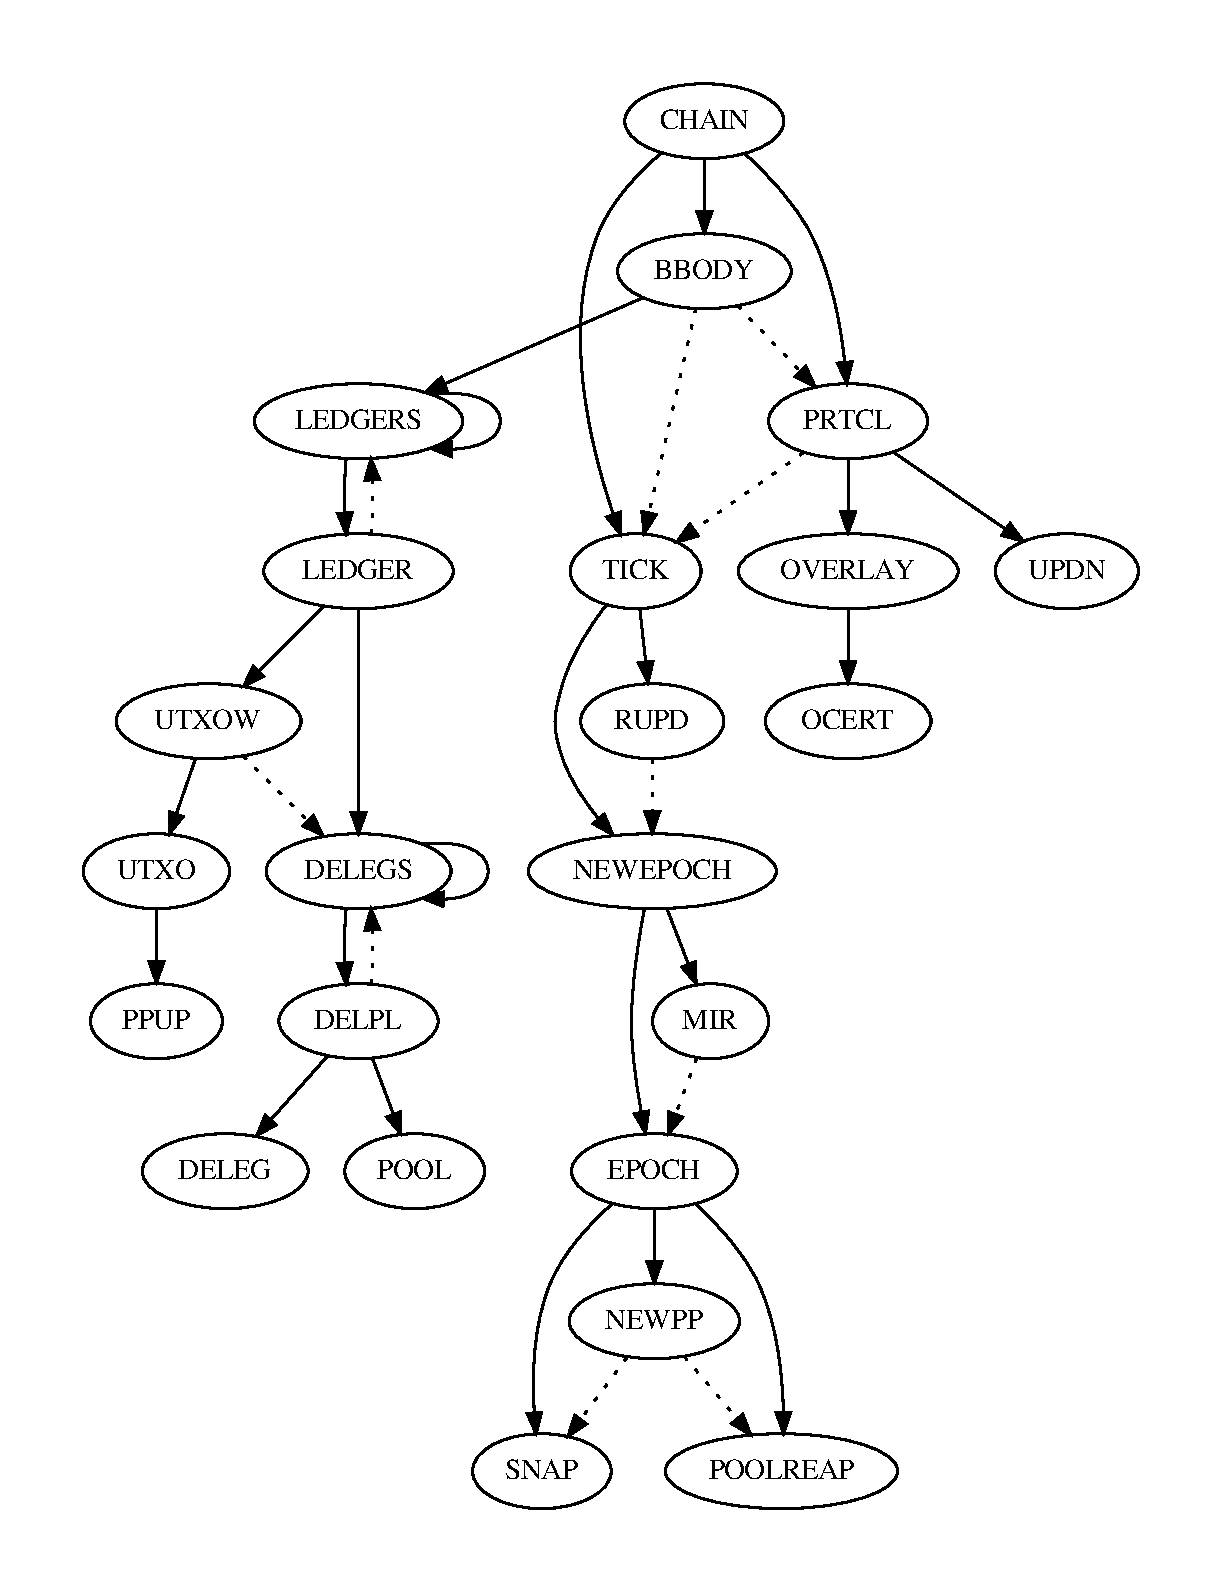
\includegraphics[width=\textwidth]{rules}
  \caption{STS Rules, Sub-Rules and Dependencies}
  \label{fig:sts-rules-dependencies}
\end{figure}

%%% Local Variables:
%%% mode: latex
%%% TeX-master: "ledger-spec"
%%% End:

\newcommand{\Val}{\fun{Val}}
\newcommand{\POV}[2]{\ensuremath{\mathsf{PresOfVal}(#1, \mathsf{#2})}}

\section{Properties}
\label{sec:properties}

The properties of this section are modifications and additions to the properties of the Shelley ledger. See \cite{shelley_spec} for definitions used here. We need to amend the definition of $\Val$ to the following:

\begin{equation*}
    \Val(x \in \Value) = x
\end{equation*}
\begin{equation*}
    \Val(x \in \Coin) = \fun{inject}~x
\end{equation*}
\begin{equation*}
    \Val((\wcard\mapsto (y \in \Value))^{*}) = \sum y
\end{equation*}

\begin{lemma}
  \label{lemma:utxo-pres-of-value}
  For all environments $e$, transactions $t$, and states $s$, $s'$, if
  \begin{equation*}
    e\vdash s\trans{utxo}{t}s'
  \end{equation*}
  then
  \begin{equation*}
    \Val(s) + wm = \Val(s')
  \end{equation*}
  where $wm = \fun{inject} (\fun{wbalance}~(\fun{txwdrls}~{t})) + \fun{mint}~(\fun{txbody}~{t})$.
\end{lemma}
\begin{proof}
  The proof is identical to the corresponding one in the previous
  specification, except that unfolding $\fun{consumed}$ gives an
  additional $\fun{mint}~{txb}$ term and all $\Coin$ quantities have
  to be converted to $\Value$.
\end{proof}

We also need to track the sum of the $\fun{mint}$ fields of all
transactions in a block, for which we write $\fun{mint}(b)$.

\begin{theorem}[Preservation of Value]
  \label{thm:chain-pres-of-value}
  For all environments $e$, blocks $b$, and states $s$, $s'$, if
  \begin{equation*}
    e\vdash s\trans{chain}{b}s'
  \end{equation*}
  then
  \begin{equation*}
    \Val(s) + \fun{mint}(b) = \Val(s')
  \end{equation*}
\end{theorem}
\begin{proof}
  Similar to the corresponding proof in the Shelley specification,
  for a given $x$ and transition $\mathsf{TR}$, let \POV{x, TR}
  be the statement:

  \begin{tabular}{l}
    for all environments $e$, signals $\sigma$, and states $s$, $s'$,
    $$
    $e\vdash s\trans{tr}{\sigma}s'~\implies~\Val(s) + x = \Val(s')$.
    $$
  \end{tabular}
  \noindent
  Then, \POV{\fun{mint}~{txb}}{LEDGER} follows from
  Lemma~\ref{lemma:utxo-pres-of-value}.  By induction, we have \\
  \POV{\fun{mint}(b)}{LEDGERS}. The rest of the proof works as
  previously, using \POV{0}{TR} or \POV{\fun{mint}(b)}{TR} as needed.
\end{proof}

\begin{theorem}[Preservation of Ada]
  \label{thm:chain-pres-of-ada}
  For all environments $e$, blocks $b$, and states $s$, $s'$, if
  \begin{equation*}
    e\vdash s\trans{chain}{b}s'
  \end{equation*}
  then
  \begin{equation*}
    \fun{coin}(\Val(s)) = \fun{coin}(\Val(s'))
  \end{equation*}
\end{theorem}
\begin{proof}
  The hypothesis implies that for all transactions $tx$ included in
  $b$, there exist some $e_{tx}, s_{tx}$ and $s'_{tx}$ such that
  $e_{tx}\vdash s_{tx}\trans{utxo}{tx}s'_{tx}$, so
  $\fun{coin}(\fun{mint}~tx) = 0$ for all transactions included
  in $b$. This implies $\fun{coin}(\fun{mint}(b)) = 0$, so the
  claim follows by Lemma~\ref{thm:chain-pres-of-value}.
\end{proof}
\section{Leader Value Calculation}
\label{sec:leader-value-calc}

This section details how we determine whether a node is entitled to lead (under
the Praos protocol) given the output of its verifiable random function
calculation.

\begin{figure}
  \emph{Values associated with the leader value calculations}
  \begin{equation*}
  \begin{array}{r@{~\in~}lr}
    \var{certNat} & \{n | n \in \N, n \in [0,2^{512})\} & \text{Certified natural value from VRF} \\
    \var{f} & [0,1] & \text{Active slot coefficient} \\
    \sigma & [0,1] & \text{Stake proportion}
  \end{array}
  \end{equation*}
\end{figure}

\subsection{Computing the leader value}

The verifiable random function gives us a 64-byte random output. We interpret
this as a natural number $\var{certNat}$ in the range $[0,2^{512})$.

\subsection{Node eligibility}

As per \cite{ouroboros_praos}, a node is eligible to lead when its leader value
$p < 1 - (1 - f)^\sigma$. We have

\begin{align*}
  p & < 1 - (1 -f)^\sigma \\
  \iff \left(\frac{1}{1-p}\right) & < \exp{(-\sigma \cdot \ln{(1-f)})}
\end{align*}

The latter inequality can be efficiently computed through use of its Taylor
expansion and error estimation to stop computing terms once we are certain that
the result will be either above or below the target value.

We carry out all computations using fixed precision arithmetic (specifically, we
use 34 decimal bits of precision, since this is enough to represent the fraction
of a single lovelace.)

As such, we define the following:

\begin{align*}
  p & = \frac{\var{certNat}}{2^{512}} \\
  q & = 1 - p \\
  c & = \ln{(1 - f)}
\end{align*}

and define the function \textit{checkLeaderVal} as follows:

\begin{equation*}
  \fun{checkLeaderVal}~\var{certNat}~\sigma~\var{f} =
    \left\{
      \begin{array}{l@{~}r}
        \mathsf{True}, & f = 1 \\
        \frac{1}{q} < \exp{(-\sigma \cdot c)}, & \text{ otherwise}
      \end{array}
    \right.
\end{equation*}

\section{Errata}
\label{sec:errata}

We list issues found within the Shelley ledger which will be corrected in future eras.

\subsection{Total stake calculation}
\label{sec:errata:total-stake}

As described in \cite[3.4.3]{delegation_design}, stake is sometimes considered
relative to all the delegated stake, and sometimes relative to the
totally supply less the amount held by the reserves.
The former is called active stake, the latter total stake.


The $\fun{createRUpd}$ function from Figure~\ref{fig:rules:reward-update} uses the
current value of the reserve pot, named $\var{reserves}$, to calculate the total stake.
It should, however, use the value of the reserve pot as it was during the previous
epoch, since $\fun{createRUpd}$ is creating the rewards earned during the previous epoch
(see the overview in Section~\ref{sec:reward-overview}).

\subsection{Active stake registrations and the Reward Calculation}
\label{sec:errata:active-accounts-and-reward-calc}

The reward calculation takes the set of active reward accounts as a parameter
(the forth parameter of $\fun{reward}$ in Figure~\ref{fig:functions:reward-calc}).
It is only used at the end of the calculation for filtering out unregistered accounts.
Therefore, if a stake credential is deregistered just before the reward calculation starts,
it cannot reregister before the end of the epoch in order to get the rewards.
The time within the epoch when the reward calculation starts should not make any difference.
Note that this does not affect the earnings that stake pools make from their margin,
since each pool's total stake is summed before filtering.
The solution is to not filter by the current active reward accounts, since rewards for
unregistered accounts go to the treasury already anyway.

\subsection{Stability Windows}
\label{sec:errata:stability-windows}

The constant $RandomnessStabilisationWindow$ was intended to be used only
for freezing the candidate nonce in the $\mathsf{UPDN}$ rule
from Figure~\ref{fig:rules:update-nonce}.
This was chosen as a good value for both Ouroboros Praos and Ouroboros Genesis.
The implementation mistakenly used the constant in the $\mathsf{RUPD}$ rule
from Figure~\ref{fig:rules:reward-update}, and used $\StabilityWindow$
in for the $\mathsf{UPDN}$ transition.

The constant $\StabilityWindow$ is a good choice for the $\mathsf{UPDN}$
transition while we remain using Ouroboros Praos, but it will be changed before
adopting Ouroboros Genesis in the consensus layer.

There is no problem with using $RandomnessStabilisationWindow$ for the
$\mathsf{RUPD}$ transition, since anything after $\StabilityWindow$ would work,
but there is no reason to do so.

\subsection{Reward aggregation}
\label{sec:errata:reward-aggregation}

On any given epoch, a reward account can earn rewards by being a member of a stake pool,
and also by being the registered reward account for a stake pool (to receive leader rewards).
A reward account can be registered to receive leader rewards from multiple stake pools.
It was intended that reward accounts receive the sum of all such rewards,
but a mistake caused reward accounts to receive at most one of them.

In Figure~\ref{fig:functions:reward-calc}, the value of $\var{potentialRewards}$ in the
$\fun{rewardOnePool}$ function should be computed using an aggregating union
$\unionoverridePlus$, so that member rewards are not overridden by leader rewards.
Similarly, the value of $\var{rewards}$ in the $\fun{reward}$ function should be computed
using an aggregating union so that leader rewards from multiple sources are aggregated.

This was corrected at the Allegra hard fork.
There were sixty-four stake addresses that were affected,
each of which was reimbursed for the exact amount lost using a MIR certificate.
Four of the stake address were unregistered and had to be re-registered.
The unregistered addresses were reimbursed in transaction
\newline
$a01b9fe136e5703668c9c7776a76cc8541b84824635d237e270670a8ca56a392$,
and the registered addresses were reimbursed in transaction
\newline
$8cab8049e3b8c4802d7d11277b21afc74056223a596c39ef00e002c2d1f507ad$.

\subsection{Byron redeem addresses}
\label{sec:errata:byron-redeem-addresses}

The bootstrap addresses from Figure~\ref{fig:defs:addresses} were not intended
to include the Byron era redeem addresses
(those with addrtype 2, see the Byron CDDL spec).
These addresses were, however, not spendable in the Shelley era.
At the Allegra hard fork they were removed from the UTxO
and the Ada contained in them was returned to the reserves.


\clearpage

\addcontentsline{toc}{section}{References}
\bibliographystyle{habbrv}
\bibliography{references}

\clearpage
\begin{appendix}
  \section{Cryptographic Details}
\label{sec:crypto-details}

\subsection{Hashing}
We present the (informal) properties of cryptographically safe hash functions:
\begin{description}
\item[Preimage resistance] It should be hard to find a message with a given hash value.
\item[Second preimage resistance] Given one message, it should be hard to find another message with the same hash value.
\item[Collision resistance] It should be hard to find two messages with the same hash value. 
\end{description}

\noindent In practice, several cryptographic protocols use hash functions as random oracles. 
However, the properties of our scheme do not depend on it.  

The hashing algorithm we use for all verification keys and multi-signature scripts is BLAKE2b-224\footnote{Note that for the signature 
and verification algorithms, as well as the proving and verification algorithms of VRFs, we use the hash function as defined in the IETF standard (see Section~\ref{sec:app-addresses} and Section~\ref{sec:app-vrf}).}.
Explicitly, this is the payment and stake credentials (Figure~\ref{fig:defs:addresses}),
the genesis keys and their delegates (Figure~\ref{fig:ts-types:pp-update}),
stake pool verification keys (Figure~\ref{fig:delegation-transitions}),
and VRF verification keys (Figure~\ref{fig:delegation-defs}). 
The only property we require of this hash function is that of Second Preimage resistance. Given the hash of verification key or multi-signature script, it should be hard to find a different key or script with the same hash. 

Everywhere else we use BLAKE2b-256. In this case we do require second preimage resistance and collision resistance. We use the output of these hash functions to produce signatures (see Figure~\ref{fig:rules:utxow-shelley}), meaning that if an adversary can find two messages with the same hash, it could break the intended EUF-CMA (Existentially UnForgeable against a Chosen Plaintext Attack) property of the underlying signature scheme. 
 
In the CDDL specification in Appendix~\ref{sec:cddl},
$\mathsf{hash28}$ refers to BLAKE2b-224 and
and $\mathsf{hash32}$ refers to BLAKE2b-256.
BLAKE2 is specified in RFC 7693 \cite{rfcBLAKE2}.

\subsection{Addresses}
\label{sec:app-addresses}
The \fun{sign} and \fun{verify} functions from Figure~\ref{fig:crypto-defs-shelley}
use Ed25519. See \cite{rfcEdDSA}.

\subsection{KES}
The \fun{sign_{ev}} and \fun{verify_{ev}} functions from Figure~\ref{fig:kes-defs-shelley}
use the iterated sum construction from Section 3.1 of \cite{cryptoeprint:2001:034}.
We allow up to $2^7$ key evolutions, which is larger than the maximum number
of evolutions allow by the spec, \MaxKESEvo, which will be set to $90$.
See Figure~\ref{fig:rules:ocert}.

\subsection{VRF}
\label{sec:app-vrf}
The \fun{verifyVrf} function from Figure~\ref{fig:defs-vrf}
uses ECVRF-ED25519-SHA512-Elligator2 as described in the draft IETF specification
\cite{rfcVRFDraft}.

More generally, we expect the following properties from a Verifyable Random Function: 
\begin{description}
\item[Full uniqueness] For any fixed public VRF key and for \textit{any} input seed, there is a unique VRF output that can be proved valid. 
\item[Full collision resistance] It should be computationally infeasible to find two distinct VRF inputs that have the same VRF output, even if the adversary knows the private key. 
\item[Pseudorandomness] Assuming the public-private key pair has been generated honestly, the VRF hash output on any adversarially-chosen VRF input looks indistinguishable from random for a computationally bounded adversary who does not know the private key. 
\end{description}

\subsection{Multi-Signatures}
As presented in Figure~\ref{fig:types-msig}, Shelley realizes multi-signatures 
in a native way, via a script-like DSL. One defines the conditions required to 
validate a multi-signature, and the script takes care of verifying the 
correctness of the request. It does so in a na\"ive way, i.e. checking every 
signature individually. For instance, if the requirement is to have $n$ valid 
signatures out of some set $\mathcal{V}$ of public keys, the na\"ive 
script-based solution checks if: (i) the number of submitted signatures is 
greater or equal to $n$, (ii) the distinct verification keys are part of the set 
$\mathcal{V}$, and (iii) at least $n$ signatures are valid. However, there are 
more efficient ways to achieve this using more advanced multi-signature schemes, 
that allow for aggregating both the signatures and the verification procedure. 
This results in less data to be stored on-chain, and a cheaper verification 
procedure. Several schemes provide these properties~\cite{musigBoneh, musig, 
musig2, pixel}, and we are currently investigating which would be the best fit 
for the Cardano ecosystem. We formally introduce multi-signature schemes.

\sloppy
A multi-signature scheme~\cite{musigs} is defined as a tuple of algorithms 
$\textsf{MS} = (\textsf{MS-Setup}, \textsf{MS-KG}, \textsf{MS-AVK}, 
\allowbreak\textsf{MS-Sign}, \textsf{MS-ASign}, \textsf{MS-Verify)}$ such that 
$\Pi\leftarrow\textsf{MS-Setup}(1^k)$ generates public parameters---where $k$ is 
the security parameter. Given the public parameters, one can generate a 
verification-signing key pair calling, 
$(\mathsf{vk,sk})\leftarrow\textsf{MS-KG}(\Pi)$. A multi-signature scheme 
provides a signing and an aggregate functionality. Mainly
\begin{itemize}
\item $\sigma\leftarrow\textsf{MS-Sign}(\Pi, \mathsf{sk}, m)$, produces a 
signature, $\sigma$, over a message $m$ using signing key $\mathsf{sk}$, and
\item $\tilde{\sigma}\leftarrow\textsf{MS-ASig}(\Pi, m, \mathcal{V, S)}$, where 
given a message $m$, a set of signatures, $\mathcal{S}$, over the message $m$, 
and the corresponding set of verification keys, $\mathcal{V}$, aggregates all 
signatures into a single, aggregate signature $\tilde{\sigma}$. 
\end{itemize}

To generate an aggregate verification key, the verifier calls the function 
$\mathsf{avk}\leftarrow\textsf{MS-AVK}(\Pi, \mathcal{V})$, which given input a 
set of verification keys, $\mathcal{V}$, returns an aggregate verification key 
that can be used for the verification of the aggregate siganture: 
$\textsf{MS-Verify}(\Pi, \mathsf{avk}, m, 
\tilde{\sigma})\in\{\textsf{true},\textsf{false}\}$. 

Note the distinction between multi-signature schemes (as described above) and 
multi-signatures as defined in Figure~\ref{fig:types-msig}. In 
Figure~\ref{fig:types-msig} we allow scripts to consider valid the 
\type{RequireAllOf}, \type{RequireAnyOf} or \type{RequireMOfN} typed signatures. 
In the definition above, given a set of public keys $\mathcal{V}$, a signature 
is considered valid if \textit{all} key owners participate. However, such 
multi-signature schemes together with a simple script-like DSL can achieve the 
properties defined in Figure~\ref{fig:types-msig} while still providing the 
benefits of a simple verification procedure, and a smaller signature size. 

  \section{Binary Address Format}
\label{sec:address-binary}

\newcommand{\binary}[1]{\ensuremath{\mathsf{#1}}}

Excepting bootstrap addresses,
the binary format for every address has a 1-byte header, followed by a payload
(bootstrap addresses use the binary encoding from the Byron era).
The header is composed of two nibbles (two 4-bit segments),
indicating the address type and the network id.

$$
\begin{array}{r@{~=~}l}
    \mathsf{address} & \mathsf{header\_byte}|\mathsf{payload} \\
                     & \mathsf{addr\_type\_nibble}|\mathsf{network\_nibble}|\mathsf{payload}
\end{array}
$$

\subsection{Header, first nibble}
\label{sec:address-binary-header-first-nibble}

The first nibble of the header specifies the type of the address.
Bootstrap addresses can also be identified by the first nibble.

\begin{center}
\begin{tabular}{ |c|c|c|c| }
 \hline
 address type & payment credential & stake credential & header, first nibble \\
 \hline
 \hline
 base address & keyhash      & keyhash    & \binary{0000} \\
 base address & scripthash   & keyhash    & \binary{0001} \\
 base address & keyhash      & scripthash & \binary{0010} \\
 base address & scripthash   & scripthash & \binary{0011} \\
 \hline
 pointer address & keyhash    & ptr & \binary{0100} \\
 pointer address & scripthash & ptr & \binary{0101} \\
 \hline
 enterprise address & keyhash    & - & \binary{0110} \\
 enterprise address & scripthash & - & \binary{0111} \\
 \hline
 bootstrap address & keyhash    & - & \binary{1000} \\
 \hline
 stake address & - & keyhash & \binary{1110} \\
 stake address & - & scripthash & \binary{1111} \\
 \hline
 future formats & ? & ? & \binary{1001}-\binary{1101} \\
 \hline
\end{tabular}
\end{center}

\subsection{Header, second nibble}
\label{sec:address-binary-header-second-nibble}

Excepting bootstrap addresses, the second nibble of the header specifies the network.

\begin{center}
\begin{tabular}{ |c|c| }
 \hline
 network & header, second nibble \\
 \hline
 \hline
 testnets & \binary{0000} \\
 mainnet & \binary{0001} \\
 future networks & \binary{0010}-\binary{1111}\\
 \hline
\end{tabular}
\end{center}

\subsection{Header, examples}
\label{sec:address-binary-header-examples}

On a \textbf{testnet},
the header for a \textbf{pointer} address whose payment credential is a \textbf{keyhash} is:
$$\binary{00000100}$$

On \textbf{mainnet}, the header for a \textbf{pointer} address whose payment credential is a \textbf{keyhash} is:
$$\binary{00010100}$$

On \textbf{mainnet}, the header for a \textbf{pointer} address whose payment credential is a \textbf{scripthash} is:
$$\binary{00010101}$$

\subsection{Payloads}
\label{sec:address-binary-payloads}

The payload for the different address types are as follows:

\begin{center}
\begin{tabular}{ |c|c| }
 \hline
 address type & payload \\
 \hline
 \hline
 base address & two 28-byte bytestrings \\
 \hline
 pointer address & one 28-byte bytestring,
 and three variable-length unsigned integers \\
 \hline
 enterprise address & one 28-byte bytestrings \\
 \hline
 stake address & one 28-byte bytestrings \\
 \hline
\end{tabular}
\end{center}

The variable-length encoding used in pointers addresses is the base-128 representation
of the number, with the the most significant bit of each byte indicating continuation.
If the significant bit is $0$, then another bytes follows.

  \section{Bootstrap Witnesses}
\label{sec:bootstrap-witnesses}

\subsection{Bootstrap Witnesses CBOR Specification}

In the Byron era of Cardano, public keys are transmitted
on chain as extended public keys as specified in \cite{bip32}.
The Shelley era of Cardano does not use extended public keys,
but does use the same cryptographic signing algorithm,
namely Ed25519.

The extended public key consists of 64 bytes,
the first 32 of which corresponds to the public key,
the second 32 of which correpsonds to something called the chain code:

$$\mathsf{extended\_pubkey} = \mathsf{pubkey}|\mathsf{chain\_code}$$

The chaincode is required for constructing bootstrap witnesses.

The CBOR specification of bootstrap witnesses,
named $\mathsf{bootstrap\_witness}$,
is given in
\url{https://github.com/input-output-hk/cardano-ledger-specs/tree/master/eras/shelley/impl/cddl-files}.

In the Shelley era, only pubkey address are supported,
and are named bootstrap addresses.

The bootstrap witness consists of the public key, the signature,
the chain code, and the address attributes.
As explained above, the public key and the signature format
are the same as for all other witnesses in the Shelley era.
The address attributes has the same format as from the Byron era address,
as specified by $\mathsf{addrattr}$ in
\url{https://github.com/input-output-hk/cardano-ledger-specs/blob/master/eras/byron/cddl-spec/byron.cddl}.


\subsection{Bootstrap Address ID Recovery}

The bootstrap address ID, named $\mathsf{addressid}$ in the Byron CDDL
specification above, can be computed as follows.

First construct the following byte string:

$$\mathsf{b} =
  \mathsf{0x830082005840}
  | \mathsf{pubkey\_bytes}
  | \mathsf{chain\_code\_bytes}
  | \mathsf{attributes\_bytes}
$$

The address ID is then obtained by first applying
sha3 256 to $\mathsf{b}$ and then applying blake2b44 to the result.
$$\mathsf{address\_id} =
  \mathsf{blake2b44}(\mathsf{sha3\_256}~\mathsf{b})
$$

  \section{CBOR Serialization Specification}
\label{sec:cddl}

Our CBOR (RFC 7049 \cite{rfcCBOR})
serialization scheme is specified using
CDDL (RFC 8610 \cite{rfcCDDL}).

The CDDL specification is located at
\url{https://github.com/input-output-hk/cardano-ledger-specs/tree/master/shelley/chain-and-ledger/shelley-spec-ledger-test/cddl-files}.

% TODO - Include the CDDL spec inline?
% \lstinputlisting[backgroundcolor = \color{lightgray}]{../executable-spec/cddl-files/shelley.cddl}

  \section{Implementation of \fun{txSize}}
\label{sec:txSize}

The minimum fee calculation in Figure~\ref{fig:defs:protocol-parameters-helpers}
depends on an abstract $\fun{txSize}$ function.
We have implemented $\fun{txSize}$ as the number of bytes in the CBOR serialization
of the transaction, as defined in Appendix~\ref{sec:cddl}.

  \section{Proofs}
\label{sec:proofs}

\newif\ifproofs
% \proofstrue comment in to include generated proofs

For the proofs we use the automated theorem prover
MetiTarski~\cite{DBLP:journals/jar/AkbarpourP10} which is specialized for proofs
over real arithmetic, including elementary functions.

\begin{proof}
The property~(\ref{prop:minimal-refund}) (p.~\pageref{prop:minimal-refund}) for
the minimal refund can be proven automatically via

\begin{verbatim}
fof(minimal_refund, conjecture,
! [Dmin, Lambda, Delta, Dval] :
((Dmin : (=0,1=) & Lambda > 0 & Delta > 0 & Dval > 0
=>
Dval*Dmin >= 0 &
(Dval * (Dmin + (1 - Dmin) * exp(-Lambda * Delta))) : (=Dval * Dmin, Dval=)))).

fof(floor_lower_upper, conjecture,
! [X] :
(X >= 0 => X - 1 <= floor(X) & floor(X) <= X)).
\end{verbatim}
  \verb|minimal_refund| shows that the resulting value is within the interval
  $[d_{val}\cdot d_{min}, d_{val}]$ and that $d_{val}\cdot d_{min}$ is
  non-negative, while \verb|floor_lower_upper| shows that the floor of a value
  $x$ has an upper bound $x$ and lower bound $x - 1$.

\ifproofs
\begin{verbatim}
SZS output start CNFRefutation for minRefund.tptp
cnf(lgen_le_neg, axiom, (X <= Y | ~ lgen(0, X, Y))).

cnf(leq_left_divide_mul_pos, axiom, (Y * Z < X | X / Z <= Y | Z <= 0)).

cnf(interval_intro, axiom,
    (~ lgen(R, A, X) | ~ lgen(S, X, B) | interval(R, A, S, B, X))).

cnf(interval_elim1, axiom, (~ interval(R, A, S, B, X) | lgen(R, A, X))).

cnf(interval_elim2, axiom, (~ interval(R, A, S, B, X) | lgen(S, X, B))).

cnf(exp_upper_bound_cf2, axiom,
    (0 <= X | ~ lgen(R, (X ^ 2 + 6 * X + 12) / (X ^ 2 - 6 * X + 12), Y) |
     lgen(R, exp(X), Y))).

fof(minimal_refund, conjecture,
    (! [Dmin, Lambda, Delta, Dval] :
       ((interval(0, 0, 0, 1, Dmin) & 0 < Lambda & 0 < Delta & 0 < Dval) =>
        (0 <= Dval * Dmin &
         interval(0, Dval * Dmin, 0, Dval,
                  Dval * (Dmin + (1 - Dmin) * exp(-Lambda * Delta))))))).

fof(subgoal_0, plain,
    (! [Dmin, Lambda, Delta, Dval] :
       ((interval(0, 0, 0, 1, Dmin) & 0 < Lambda & 0 < Delta & 0 < Dval) =>
        0 <= Dval * Dmin)), inference(strip, [], [minimal_refund])).

fof(subgoal_1, plain,
    (! [Dmin, Lambda, Delta, Dval] :
       (((interval(0, 0, 0, 1, Dmin) & 0 < Lambda & 0 < Delta & 0 < Dval) &
         0 <= Dval * Dmin) =>
        interval(0, Dval * Dmin, 0, Dval,
                 Dval * (Dmin + (1 - Dmin) * exp(-Lambda * Delta))))),
    inference(strip, [], [minimal_refund])).

fof(negate_0_0, plain,
    (~ ! [Dmin, Lambda, Delta, Dval] :
         ((interval(0, 0, 0, 1, Dmin) & 0 < Lambda & 0 < Delta &
           0 < Dval) => 0 <= Dval * Dmin)),
    inference(negate, [], [subgoal_0])).

fof(normalize_0_0, plain,
    (? [Delta, Dmin, Dval, Lambda] :
       (0 < Delta & 0 < Dval & 0 < Lambda & Dval * Dmin < 0 &
        interval(0, 0, 0, 1, Dmin))),
    inference(canonicalize, [], [negate_0_0])).

fof(normalize_0_1, plain,
    (skoDvalC2 * skoDminC2 < 0 & 0 < skoDeltaC2 & 0 < skoDvalC2 &
     0 < skoLambdaC2 & interval(0, 0, 0, 1, skoDminC2)),
    inference(skolemize, [], [normalize_0_0])).

fof(normalize_0_2, plain, (interval(0, 0, 0, 1, skoDminC2)),
    inference(conjunct, [], [normalize_0_1])).

fof(normalize_0_3, plain, (skoDvalC2 * skoDminC2 < 0),
    inference(conjunct, [], [normalize_0_1])).

fof(normalize_0_4, plain, (0 < skoLambdaC2),
    inference(conjunct, [], [normalize_0_1])).

fof(normalize_0_5, plain, (0 < skoDvalC2),
    inference(conjunct, [], [normalize_0_1])).

fof(normalize_0_6, plain, (0 < skoDeltaC2),
    inference(conjunct, [], [normalize_0_1])).

cnf(refute_0_0, plain, (interval(0, 0, 0, 1, skoDminC2)),
    inference(canonicalize, [], [normalize_0_2])).

cnf(refute_0_1, plain,
    (~ interval(0, 0, 0, 1, skoDminC2) | lgen(0, 0, skoDminC2)),
    inference(subst, [], [interval_elim1])).

cnf(refute_0_2, plain, (lgen(0, 0, skoDminC2)),
    inference(resolve, [], [refute_0_0, refute_0_1])).

cnf(refute_0_3, plain, (0 <= skoDminC2),
    inference(arithmetic, [], [refute_0_2])).

cnf(refute_0_4, plain, (skoDvalC2 * skoDminC2 < 0),
    inference(canonicalize, [], [normalize_0_3])).

cnf(refute_0_5, plain, (0 < skoDvalC2 * (skoDminC2 * -1)),
    inference(arithmetic, [], [refute_0_4])).

cnf(refute_0_6, plain, (0 < skoLambdaC2),
    inference(canonicalize, [], [normalize_0_4])).

cnf(refute_0_7, plain, (0 < skoDvalC2),
    inference(canonicalize, [], [normalize_0_5])).

cnf(refute_0_8, plain, (0 < skoDeltaC2),
    inference(canonicalize, [], [normalize_0_6])).

cnf(refute_0_9, plain, (skoDminC2 < 0),
    inference(decision, [],
              [refute_0_5, refute_0_6, refute_0_7, refute_0_8])).

cnf(refute_0_10, plain, ($false),
    inference(resolve, [], [refute_0_3, refute_0_9])).

fof(negate_1_0, plain,
    (~ ! [Dmin, Lambda, Delta, Dval] :
         (((interval(0, 0, 0, 1, Dmin) & 0 < Lambda & 0 < Delta &
            0 < Dval) & 0 <= Dval * Dmin) =>
          interval(0, Dval * Dmin, 0, Dval,
                   Dval * (Dmin + (1 - Dmin) * exp(-Lambda * Delta))))),
    inference(negate, [], [subgoal_1])).

fof(normalize_1_0, plain,
    (? [Delta, Dmin, Dval, Lambda] :
       (0 < Delta & 0 < Dval & 0 < Lambda &
        ~ interval(0, Dval * Dmin, 0, Dval,
                   Dval * (Dmin + (1 - Dmin) * exp(-Lambda * Delta))) &
        0 <= Dval * Dmin & interval(0, 0, 0, 1, Dmin))),
    inference(canonicalize, [], [negate_1_0])).

fof(normalize_1_1, plain,
    (0 < skoDeltaC3 & 0 < skoDvalC3 & 0 < skoLambdaC3 &
     ~ interval(0, skoDvalC3 * skoDminC3, 0, skoDvalC3,
                skoDvalC3 *
                (skoDminC3 +
                 (1 - skoDminC3) * exp(-skoLambdaC3 * skoDeltaC3))) &
     0 <= skoDvalC3 * skoDminC3 & interval(0, 0, 0, 1, skoDminC3)),
    inference(skolemize, [], [normalize_1_0])).

fof(normalize_1_2, plain,
    (~ interval(0, skoDvalC3 * skoDminC3, 0, skoDvalC3,
                skoDvalC3 *
                (skoDminC3 +
                 (1 - skoDminC3) * exp(-skoLambdaC3 * skoDeltaC3)))),
    inference(conjunct, [], [normalize_1_1])).

fof(normalize_1_3, plain, (interval(0, 0, 0, 1, skoDminC3)),
    inference(conjunct, [], [normalize_1_1])).

fof(normalize_1_4, plain, (0 <= skoDvalC3 * skoDminC3),
    inference(conjunct, [], [normalize_1_1])).

fof(normalize_1_5, plain, (0 < skoLambdaC3),
    inference(conjunct, [], [normalize_1_1])).

fof(normalize_1_6, plain, (0 < skoDvalC3),
    inference(conjunct, [], [normalize_1_1])).

fof(normalize_1_7, plain, (0 < skoDeltaC3),
    inference(conjunct, [], [normalize_1_1])).

cnf(refute_1_0, plain,
    (1 *
     (12 +
      skoLambdaC3 *
      (skoDeltaC3 * 6 + skoLambdaC3 * (skoDeltaC3 * skoDeltaC3))) <
     12 +
     skoLambdaC3 *
     (skoDeltaC3 * -6 + skoLambdaC3 * (skoDeltaC3 * skoDeltaC3)) |
     12 +
     skoLambdaC3 *
     (skoDeltaC3 * 6 + skoLambdaC3 * (skoDeltaC3 * skoDeltaC3)) <= 0 |
     (12 +
      skoLambdaC3 *
      (skoDeltaC3 * -6 + skoLambdaC3 * (skoDeltaC3 * skoDeltaC3))) /
     (12 +
      skoLambdaC3 *
      (skoDeltaC3 * 6 + skoLambdaC3 * (skoDeltaC3 * skoDeltaC3))) <= 1),
    inference(subst, [], [leq_left_divide_mul_pos])).

cnf(refute_1_1, plain,
    (~ lgen(0, exp(X_000190), X_000191) | exp(X_000190) <= X_000191),
    inference(subst, [], [lgen_le_neg])).

cnf(refute_1_2, plain,
    (~ lgen(0,
            (X_000190 ^ 2 + 6 * X_000190 + 12) /
            (X_000190 ^ 2 - 6 * X_000190 + 12), X_000191) | 0 <= X_000190 |
     lgen(0, exp(X_000190), X_000191)),
    inference(subst, [], [exp_upper_bound_cf2])).

cnf(refute_1_3, plain,
    (~ lgen(0,
            (X_000190 ^ 2 + 6 * X_000190 + 12) /
            (X_000190 ^ 2 - 6 * X_000190 + 12), X_000191) | 0 <= X_000190 |
     exp(X_000190) <= X_000191),
    inference(resolve, [], [refute_1_2, refute_1_1])).

cnf(refute_1_4, plain,
    (X_000191 <
     (12 + X_000190 * (6 + X_000190)) / (12 + X_000190 * (-6 + X_000190)) |
     0 <= X_000190 | exp(X_000190) <= X_000191),
    inference(arithmetic, [], [refute_1_3])).

cnf(refute_1_5, plain,
    (1 <
     (12 +
      skoLambdaC3 * (skoDeltaC3 * -1) *
      (6 + skoLambdaC3 * (skoDeltaC3 * -1))) /
     (12 +
      skoLambdaC3 * (skoDeltaC3 * -1) *
      (-6 + skoLambdaC3 * (skoDeltaC3 * -1))) |
     0 <= skoLambdaC3 * (skoDeltaC3 * -1) |
     exp(skoLambdaC3 * (skoDeltaC3 * -1)) <= 1),
    inference(subst, [], [refute_1_4])).

cnf(refute_1_6, plain,
    (~ interval(0, skoDvalC3 * skoDminC3, 0, skoDvalC3,
                skoDvalC3 *
                (skoDminC3 +
                 (1 - skoDminC3) * exp(-skoLambdaC3 * skoDeltaC3)))),
    inference(canonicalize, [], [normalize_1_2])).

cnf(refute_1_7, plain,
    (~ interval(0, skoDvalC3 * skoDminC3, 0, skoDvalC3,
                skoDvalC3 * skoDminC3 +
                exp(skoLambdaC3 * (skoDeltaC3 * -1)) *
                (skoDvalC3 * (1 + skoDminC3 * -1)))),
    inference(arithmetic, [], [refute_1_6])).

cnf(refute_1_8, plain,
    (~ lgen(0, skoDvalC3 * skoDminC3,
            skoDvalC3 * skoDminC3 +
            exp(skoLambdaC3 * (skoDeltaC3 * -1)) *
            (skoDvalC3 * (1 + skoDminC3 * -1))) |
     ~ lgen(0,
            skoDvalC3 * skoDminC3 +
            exp(skoLambdaC3 * (skoDeltaC3 * -1)) *
            (skoDvalC3 * (1 + skoDminC3 * -1)), skoDvalC3) |
     interval(0, skoDvalC3 * skoDminC3, 0, skoDvalC3,
              skoDvalC3 * skoDminC3 +
              exp(skoLambdaC3 * (skoDeltaC3 * -1)) *
              (skoDvalC3 * (1 + skoDminC3 * -1)))),
    inference(subst, [], [interval_intro])).

cnf(refute_1_9, plain,
    (~ lgen(0, skoDvalC3 * skoDminC3,
            skoDvalC3 * skoDminC3 +
            exp(skoLambdaC3 * (skoDeltaC3 * -1)) *
            (skoDvalC3 * (1 + skoDminC3 * -1))) |
     ~ lgen(0,
            skoDvalC3 * skoDminC3 +
            exp(skoLambdaC3 * (skoDeltaC3 * -1)) *
            (skoDvalC3 * (1 + skoDminC3 * -1)), skoDvalC3)),
    inference(resolve, [], [refute_1_8, refute_1_7])).

cnf(refute_1_10, plain,
    (0 <
     exp(skoLambdaC3 * (skoDeltaC3 * -1)) *
     (skoDvalC3 * (-1 + skoDminC3)) |
     skoDvalC3 * (1 + skoDminC3 * -1) <
     exp(skoLambdaC3 * (skoDeltaC3 * -1)) *
     (skoDvalC3 * (1 + skoDminC3 * -1))),
    inference(arithmetic, [], [refute_1_9])).

cnf(refute_1_11, plain,
    (0 <
     exp(skoLambdaC3 * (skoDeltaC3 * -1)) *
     (skoDvalC3 * (-1 + skoDminC3)) |
     exp(skoLambdaC3 * (skoDeltaC3 * -1)) *
     (skoDvalC3 * (-1 + skoDminC3)) <= 0),
    introduced(tautology, [assume])).

cnf(refute_1_12, plain,
    (0 < 0 | skoDvalC3 * (-1 + skoDminC3) < 0 |
     0 < skoDvalC3 * (-1 + skoDminC3) |
     exp(skoLambdaC3 * (skoDeltaC3 * -1)) *
     (skoDvalC3 * (-1 + skoDminC3)) <= 0),
    inference(split, [], [refute_1_11])).

cnf(refute_1_13, plain,
    (0 < skoDvalC3 * (-1 + skoDminC3) |
     0 < skoDvalC3 * (1 + skoDminC3 * -1) |
     exp(skoLambdaC3 * (skoDeltaC3 * -1)) *
     (skoDvalC3 * (-1 + skoDminC3)) <= 0),
    inference(arithmetic, [], [refute_1_12])).

cnf(refute_1_14, plain,
    (exp(skoLambdaC3 * (skoDeltaC3 * -1)) <
     0 / (skoDvalC3 * (-1 + skoDminC3)) |
     0 <= skoDvalC3 * (-1 + skoDminC3) |
     exp(skoLambdaC3 * (skoDeltaC3 * -1)) *
     (skoDvalC3 * (-1 + skoDminC3)) <= 0),
    inference(split, [], [refute_1_11])).

cnf(refute_1_15, plain,
    (exp(skoLambdaC3 * (skoDeltaC3 * -1)) *
     (skoDvalC3 * (-1 + skoDminC3)) <= 0 |
     skoDvalC3 * (1 + skoDminC3 * -1) <= 0),
    inference(arithmetic, [], [refute_1_14])).

cnf(refute_1_16, plain,
    (0 < skoDvalC3 * (-1 + skoDminC3) |
     exp(skoLambdaC3 * (skoDeltaC3 * -1)) *
     (skoDvalC3 * (-1 + skoDminC3)) <= 0),
    inference(resolve, [], [refute_1_15, refute_1_13])).

cnf(refute_1_17, plain, (interval(0, 0, 0, 1, skoDminC3)),
    inference(canonicalize, [], [normalize_1_3])).

cnf(refute_1_18, plain,
    (~ interval(0, 0, 0, 1, skoDminC3) | lgen(0, skoDminC3, 1)),
    inference(subst, [], [interval_elim2])).

cnf(refute_1_19, plain, (lgen(0, skoDminC3, 1)),
    inference(resolve, [], [refute_1_17, refute_1_18])).

cnf(refute_1_20, plain, (skoDminC3 <= 1),
    inference(arithmetic, [], [refute_1_19])).

cnf(refute_1_21, plain, (0 <= skoDvalC3 * skoDminC3),
    inference(canonicalize, [], [normalize_1_4])).

cnf(refute_1_22, plain, (skoDvalC3 * (skoDminC3 * -1) <= 0),
    inference(arithmetic, [], [refute_1_21])).

cnf(refute_1_23, plain, (0 < skoLambdaC3),
    inference(canonicalize, [], [normalize_1_5])).

cnf(refute_1_24, plain, (0 < skoDvalC3),
    inference(canonicalize, [], [normalize_1_6])).

cnf(refute_1_25, plain, (0 < skoDeltaC3),
    inference(canonicalize, [], [normalize_1_7])).

cnf(refute_1_26, plain, (skoDvalC3 * (-1 + skoDminC3) <= 0),
    inference(decision, [],
              [refute_1_20, refute_1_22, refute_1_23, refute_1_24,
               refute_1_25])).

cnf(refute_1_27, plain,
    (exp(skoLambdaC3 * (skoDeltaC3 * -1)) *
     (skoDvalC3 * (-1 + skoDminC3)) <= 0),
    inference(resolve, [], [refute_1_26, refute_1_16])).

cnf(refute_1_28, plain,
    (skoDvalC3 * (1 + skoDminC3 * -1) <
     exp(skoLambdaC3 * (skoDeltaC3 * -1)) *
     (skoDvalC3 * (1 + skoDminC3 * -1))),
    inference(resolve, [], [refute_1_27, refute_1_10])).

cnf(refute_1_29, plain,
    (skoDvalC3 * (1 + skoDminC3 * -1) /
     (skoDvalC3 * (1 + skoDminC3 * -1)) <
     exp(skoLambdaC3 * (skoDeltaC3 * -1)) |
     skoDvalC3 * (1 + skoDminC3 * -1) <= 0),
    inference(split, [], [refute_1_28])).

cnf(refute_1_30, plain,
    (1 < exp(skoLambdaC3 * (skoDeltaC3 * -1)) |
     skoDvalC3 * (1 + skoDminC3 * -1) <= 0 | 1 = skoDminC3 |
     skoDvalC3 = 0), inference(arithmetic, [], [refute_1_29])).

cnf(refute_1_31, plain,
    (0 < skoDvalC3 * (1 + skoDminC3 * -1) | 1 = skoDminC3 | skoDvalC3 = 0),
    inference(decision, [],
              [refute_1_25, refute_1_24, refute_1_23, refute_1_22,
               refute_1_20])).

cnf(refute_1_32, plain,
    (1 < exp(skoLambdaC3 * (skoDeltaC3 * -1)) | 1 = skoDminC3 |
     skoDvalC3 = 0), inference(resolve, [], [refute_1_30, refute_1_31])).

cnf(refute_1_33, plain, (skoDvalC3 != 0 | 1 = skoDminC3),
    inference(decision, [],
              [refute_1_25, refute_1_24, refute_1_23, refute_1_22,
               refute_1_20])).

cnf(refute_1_34, plain,
    (1 < exp(skoLambdaC3 * (skoDeltaC3 * -1)) | 1 = skoDminC3),
    inference(resolve, [], [refute_1_32, refute_1_33])).

cnf(refute_1_35, plain,
    (1 <
     (12 +
      skoLambdaC3 * (skoDeltaC3 * -1) *
      (6 + skoLambdaC3 * (skoDeltaC3 * -1))) /
     (12 +
      skoLambdaC3 * (skoDeltaC3 * -1) *
      (-6 + skoLambdaC3 * (skoDeltaC3 * -1))) |
     0 <= skoLambdaC3 * (skoDeltaC3 * -1) | 1 = skoDminC3),
    inference(resolve, [], [refute_1_5, refute_1_34])).

cnf(refute_1_36, plain,
    (1 <
     (12 +
      skoLambdaC3 *
      (skoDeltaC3 * -6 + skoLambdaC3 * (skoDeltaC3 * skoDeltaC3))) /
     (12 +
      skoLambdaC3 *
      (skoDeltaC3 * 6 + skoLambdaC3 * (skoDeltaC3 * skoDeltaC3))) |
     skoLambdaC3 * skoDeltaC3 <= 0 | 1 = skoDminC3),
    inference(arithmetic, [], [refute_1_35])).

cnf(refute_1_37, plain,
    (skoDvalC3 * (1 + skoDminC3 * -1) < 0 |
     0 < skoDvalC3 * (1 + skoDminC3 * -1)),
    inference(split, [], [refute_1_28])).

cnf(refute_1_38, plain,
    (0 < skoDvalC3 * (-1 + skoDminC3) |
     0 < skoDvalC3 * (1 + skoDminC3 * -1)),
    inference(arithmetic, [], [refute_1_37])).

cnf(refute_1_39, plain,
    (0 < skoDvalC3 * (1 + skoDminC3 * -1) |
     skoDvalC3 * (-1 + skoDminC3) <= 0),
    inference(decision, [],
              [refute_1_25, refute_1_24, refute_1_23, refute_1_22,
               refute_1_20])).

cnf(refute_1_40, plain, (0 < skoDvalC3 * (1 + skoDminC3 * -1)),
    inference(resolve, [], [refute_1_39, refute_1_38])).

cnf(refute_1_41, plain, (0 < skoLambdaC3 * skoDeltaC3 | 1 = skoDminC3),
    inference(decision, [],
              [refute_1_40, refute_1_25, refute_1_24, refute_1_23,
               refute_1_22, refute_1_20])).

cnf(refute_1_42, plain,
    (1 <
     (12 +
      skoLambdaC3 *
      (skoDeltaC3 * -6 + skoLambdaC3 * (skoDeltaC3 * skoDeltaC3))) /
     (12 +
      skoLambdaC3 *
      (skoDeltaC3 * 6 + skoLambdaC3 * (skoDeltaC3 * skoDeltaC3))) |
     1 = skoDminC3), inference(resolve, [], [refute_1_36, refute_1_41])).

cnf(refute_1_43, plain, (1 != skoDminC3),
    inference(decision, [],
              [refute_1_40, refute_1_25, refute_1_24, refute_1_23,
               refute_1_22, refute_1_20])).

cnf(refute_1_44, plain,
    (1 <
     (12 +
      skoLambdaC3 *
      (skoDeltaC3 * -6 + skoLambdaC3 * (skoDeltaC3 * skoDeltaC3))) /
     (12 +
      skoLambdaC3 *
      (skoDeltaC3 * 6 + skoLambdaC3 * (skoDeltaC3 * skoDeltaC3)))),
    inference(resolve, [], [refute_1_42, refute_1_43])).

cnf(refute_1_45, plain,
    (1 *
     (12 +
      skoLambdaC3 *
      (skoDeltaC3 * 6 + skoLambdaC3 * (skoDeltaC3 * skoDeltaC3))) <
     12 +
     skoLambdaC3 *
     (skoDeltaC3 * -6 + skoLambdaC3 * (skoDeltaC3 * skoDeltaC3)) |
     12 +
     skoLambdaC3 *
     (skoDeltaC3 * 6 + skoLambdaC3 * (skoDeltaC3 * skoDeltaC3)) <= 0),
    inference(resolve, [], [refute_1_0, refute_1_44])).

cnf(refute_1_46, plain,
    (0 < skoLambdaC3 * (skoDeltaC3 * -12) |
     skoLambdaC3 *
     (skoDeltaC3 * 6 + skoLambdaC3 * (skoDeltaC3 * skoDeltaC3)) <= -12),
    inference(arithmetic, [], [refute_1_45])).

cnf(refute_1_47, plain,
    (0 < skoLambdaC3 * (skoDeltaC3 * -12) |
     -12 <
     skoLambdaC3 *
     (skoDeltaC3 * 6 + skoLambdaC3 * (skoDeltaC3 * skoDeltaC3))),
    inference(decision, [],
              [refute_1_40, refute_1_25, refute_1_24, refute_1_23,
               refute_1_22, refute_1_20])).

cnf(refute_1_48, plain, (0 < skoLambdaC3 * (skoDeltaC3 * -12)),
    inference(resolve, [], [refute_1_46, refute_1_47])).

cnf(refute_1_49, plain, (skoLambdaC3 * (skoDeltaC3 * -12) <= 0),
    inference(decision, [],
              [refute_1_40, refute_1_25, refute_1_24, refute_1_23,
               refute_1_22, refute_1_20])).

cnf(refute_1_50, plain, ($false),
    inference(resolve, [], [refute_1_49, refute_1_48])).
SZS output end CNFRefutation for minRefund.tptp
\end{verbatim}

\begin{verbatim}
SZS output start CNFRefutation for floor.tptp
cnf(lgen_le_neg, axiom, (X <= Y | ~ lgen(0, X, Y))).

cnf(floor_upper_bound, axiom, (~ lgen(R, X, Y) | lgen(R, floor(X), Y))).

cnf(floor_lower_bound, axiom, (X - 1 < Y | lgen(R, Y, floor(X)))).

fof(floor_lower_upper, conjecture,
    (! [X] : (0 <= X => (X - 1 <= floor(X) & floor(X) <= X)))).

fof(subgoal_0, plain, (! [X] : (0 <= X => X - 1 <= floor(X))),
    inference(strip, [], [floor_lower_upper])).

fof(subgoal_1, plain,
    (! [X] : ((0 <= X & X - 1 <= floor(X)) => floor(X) <= X)),
    inference(strip, [], [floor_lower_upper])).

fof(negate_0_0, plain, (~ ! [X] : (0 <= X => X - 1 <= floor(X))),
    inference(negate, [], [subgoal_0])).

fof(normalize_0_0, plain, (? [X] : (floor(X) < X - 1 & 0 <= X)),
    inference(canonicalize, [], [negate_0_0])).

fof(normalize_0_1, plain, (floor(skoXC2) < skoXC2 - 1 & 0 <= skoXC2),
    inference(skolemize, [], [normalize_0_0])).

fof(normalize_0_2, plain, (floor(skoXC2) < skoXC2 - 1),
    inference(conjunct, [], [normalize_0_1])).

cnf(refute_0_0, plain, (floor(skoXC2) < skoXC2 - 1),
    inference(canonicalize, [], [normalize_0_2])).

cnf(refute_0_1, plain, (floor(skoXC2) < -1 + skoXC2),
    inference(arithmetic, [], [refute_0_0])).

cnf(refute_0_2, plain,
    (~ lgen(0, X_000012, floor(X_000011)) | X_000012 <= floor(X_000011)),
    inference(subst, [], [lgen_le_neg])).

cnf(refute_0_3, plain,
    (X_000011 - 1 < X_000012 | lgen(0, X_000012, floor(X_000011))),
    inference(subst, [], [floor_lower_bound])).

cnf(refute_0_4, plain,
    (X_000011 - 1 < X_000012 | X_000012 <= floor(X_000011)),
    inference(resolve, [], [refute_0_3, refute_0_2])).

cnf(refute_0_5, plain,
    (-1 + X_000011 < X_000012 | X_000012 <= floor(X_000011)),
    inference(arithmetic, [], [refute_0_4])).

cnf(refute_0_6, plain,
    (-1 + skoXC2 < -1 + skoXC2 | -1 + skoXC2 <= floor(skoXC2)),
    inference(subst, [], [refute_0_5])).

cnf(refute_0_7, plain, (-1 + skoXC2 < -1 + skoXC2),
    inference(resolve, [], [refute_0_6, refute_0_1])).

cnf(refute_0_8, plain, ($false), inference(arithmetic, [], [refute_0_7])).

fof(negate_1_0, plain,
    (~ ! [X] : ((0 <= X & X - 1 <= floor(X)) => floor(X) <= X)),
    inference(negate, [], [subgoal_1])).

fof(normalize_1_0, plain,
    (? [X] : (X < floor(X) & 0 <= X & X - 1 <= floor(X))),
    inference(canonicalize, [], [negate_1_0])).

fof(normalize_1_1, plain,
    (skoXC3 < floor(skoXC3) & 0 <= skoXC3 & skoXC3 - 1 <= floor(skoXC3)),
    inference(skolemize, [], [normalize_1_0])).

fof(normalize_1_2, plain, (skoXC3 < floor(skoXC3)),
    inference(conjunct, [], [normalize_1_1])).

cnf(refute_1_0, plain, (skoXC3 < floor(skoXC3)),
    inference(canonicalize, [], [normalize_1_2])).

cnf(refute_1_1, plain,
    (~ lgen(0, floor(X_000034), X_000035) | floor(X_000034) <= X_000035),
    inference(subst, [], [lgen_le_neg])).

cnf(refute_1_2, plain,
    (~ lgen(0, X_000034, X_000035) | lgen(0, floor(X_000034), X_000035)),
    inference(subst, [], [floor_upper_bound])).

cnf(refute_1_3, plain,
    (~ lgen(0, X_000034, X_000035) | floor(X_000034) <= X_000035),
    inference(resolve, [], [refute_1_2, refute_1_1])).

cnf(refute_1_4, plain, (X_000035 < X_000034 | floor(X_000034) <= X_000035),
    inference(arithmetic, [], [refute_1_3])).

cnf(refute_1_5, plain, (skoXC3 < skoXC3 | floor(skoXC3) <= skoXC3),
    inference(subst, [], [refute_1_4])).

cnf(refute_1_6, plain, (skoXC3 < skoXC3),
    inference(resolve, [], [refute_1_5, refute_1_0])).

cnf(refute_1_7, plain, ($false), inference(arithmetic, [], [refute_1_6])).
SZS output end CNFRefutation for floor.tptp
\end{verbatim}
\fi
\end{proof}


\begin{proof}
  For the property~(\ref{prop:reward-splitting})
  (p.~\pageref{prop:reward-splitting}) for reward splitting we actually show a
  stronger one, by removing the floor function. Using the fractional values we
  get an upper bound for the real value and showing that this upper bound is
  bounded by $\hat{f}$ we show that the real value is also bounded by
  $\hat{f}$. To eliminate the sum, we use the identity $\frac{s +
    \sum_{j}t_{j}}{\sigma} = 1$, see the definition of
  $\sigma$ in~\cite{delegation_design}. Using this, we show for $\hat{f} > c$

  \begin{equation*}
    \begin{array}{cll}
      & 0 \leq c + (\hat{f} - c)\cdot (m + (1 - m))\cdot \frac{s}{\sigma} +
        \sum_{j}(\hat{f}-c)\cdot(1-m)\cdot\frac{t_{j}}{\sigma} & \leq \hat{f} \\
      \Leftrightarrow &
                        0\leq c + (\hat{f}-c)\cdot m \cdot \frac{s}{\sigma} + (\hat{f}
                        -c)\cdot(1-m)\cdot\frac{s + \sum_{j}t_{j}}{\sigma} & \leq \hat{f} \\
      \Leftrightarrow &
                        0\leq c + (\hat{f}-c)\cdot m \cdot \frac{s}{\sigma} + (\hat{f}
                        -c)\cdot(1-m) & \leq \hat{f} \\
    \end{array}
  \end{equation*}

  This can be proven automatically using

\begin{verbatim}
fof(reward_splitting, conjecture,
! [C, F, M, S, Sigma] :
(
M : (=0, 1=) & C >= 0 & F > C & Sigma : (0, 1=) & S : (=0, Sigma=)
=>
C + (F - C) * M * S / Sigma + (F - C) * (1 - M) <= F &
0 <= C + (F - C) * M * S / Sigma + (F - C) * (1 - M))).
\end{verbatim}

  \ifproofs
\begin{verbatim}
SZS output start CNFRefutation for rewardsplit.tptp
cnf(leq_left_divide_mul_pos, axiom, (Y * Z < X | X / Z <= Y | Z <= 0)).

cnf(leq_right_divide_mul_pos, axiom, (Y < X * Z | X <= Y / Z | Z <= 0)).

cnf(leq_left_divide_mul_neg, axiom, (Y * Z < X | Y <= X / Z | 0 <= Z)).

cnf(leq_right_divide_mul_neg, axiom, (Y < X * Z | Y / Z <= X | 0 <= Z)).

cnf(interval_elim1, axiom, (~ interval(R, A, S, B, X) | lgen(R, A, X))).

cnf(interval_elim2, axiom, (~ interval(R, A, S, B, X) | lgen(S, X, B))).

fof(reward_splitting, conjecture,
    (! [C, F, M, S, Sigma] :
       ((interval(0, 0, 0, 1, M) & 0 <= C & C < F &
         interval(1, 0, 0, 1, Sigma) & interval(0, 0, 0, Sigma, S)) =>
        (C + (F - C) * M * S / Sigma + (F - C) * (1 - M) <= F &
         0 <= C + (F - C) * M * S / Sigma + (F - C) * (1 - M))))).

fof(subgoal_0, plain,
    (! [C, F, M, S, Sigma] :
       ((interval(0, 0, 0, 1, M) & 0 <= C & C < F &
         interval(1, 0, 0, 1, Sigma) & interval(0, 0, 0, Sigma, S)) =>
        C + (F - C) * M * S / Sigma + (F - C) * (1 - M) <= F)),
    inference(strip, [], [reward_splitting])).

fof(subgoal_1, plain,
    (! [C, F, M, S, Sigma] :
       (((interval(0, 0, 0, 1, M) & 0 <= C & C < F &
          interval(1, 0, 0, 1, Sigma) & interval(0, 0, 0, Sigma, S)) &
         C + (F - C) * M * S / Sigma + (F - C) * (1 - M) <= F) =>
        0 <= C + (F - C) * M * S / Sigma + (F - C) * (1 - M))),
    inference(strip, [], [reward_splitting])).

fof(negate_0_0, plain,
    (~ ! [C, F, M, S, Sigma] :
         ((interval(0, 0, 0, 1, M) & 0 <= C & C < F &
           interval(1, 0, 0, 1, Sigma) & interval(0, 0, 0, Sigma, S)) =>
          C + (F - C) * M * S / Sigma + (F - C) * (1 - M) <= F)),
    inference(negate, [], [subgoal_0])).

fof(normalize_0_0, plain,
    (? [C, F, M, S, Sigma] :
       (C < F & F < C + (F - C) * M * S / Sigma + (F - C) * (1 - M) &
        0 <= C & interval(0, 0, 0, Sigma, S) & interval(0, 0, 0, 1, M) &
        interval(1, 0, 0, 1, Sigma))),
    inference(canonicalize, [], [negate_0_0])).

fof(normalize_0_1, plain,
    (skoFC2 <
     skoCC2 + (skoFC2 - skoCC2) * skoMC2 * skoSC2 / skoSigmaC2 +
     (skoFC2 - skoCC2) * (1 - skoMC2) & skoCC2 < skoFC2 & 0 <= skoCC2 &
     interval(0, 0, 0, 1, skoMC2) & interval(0, 0, 0, skoSigmaC2, skoSC2) &
     interval(1, 0, 0, 1, skoSigmaC2)),
    inference(skolemize, [], [normalize_0_0])).

fof(normalize_0_2, plain, (interval(0, 0, 0, skoSigmaC2, skoSC2)),
    inference(conjunct, [], [normalize_0_1])).

fof(normalize_0_3, plain, (interval(1, 0, 0, 1, skoSigmaC2)),
    inference(conjunct, [], [normalize_0_1])).

fof(normalize_0_4, plain, (interval(0, 0, 0, 1, skoMC2)),
    inference(conjunct, [], [normalize_0_1])).

fof(normalize_0_5, plain,
    (skoFC2 <
     skoCC2 + (skoFC2 - skoCC2) * skoMC2 * skoSC2 / skoSigmaC2 +
     (skoFC2 - skoCC2) * (1 - skoMC2)),
    inference(conjunct, [], [normalize_0_1])).

fof(normalize_0_6, plain, (0 <= skoCC2),
    inference(conjunct, [], [normalize_0_1])).

fof(normalize_0_7, plain, (skoCC2 < skoFC2),
    inference(conjunct, [], [normalize_0_1])).

cnf(refute_0_0, plain, (interval(0, 0, 0, skoSigmaC2, skoSC2)),
    inference(canonicalize, [], [normalize_0_2])).

cnf(refute_0_1, plain,
    (~ interval(0, 0, 0, skoSigmaC2, skoSC2) |
     lgen(0, skoSC2, skoSigmaC2)), inference(subst, [], [interval_elim2])).

cnf(refute_0_2, plain, (lgen(0, skoSC2, skoSigmaC2)),
    inference(resolve, [], [refute_0_0, refute_0_1])).

cnf(refute_0_3, plain, (skoSC2 <= skoSigmaC2),
    inference(arithmetic, [], [refute_0_2])).

cnf(refute_0_4, plain, (interval(1, 0, 0, 1, skoSigmaC2)),
    inference(canonicalize, [], [normalize_0_3])).

cnf(refute_0_5, plain,
    (~ interval(1, 0, 0, 1, skoSigmaC2) | lgen(1, 0, skoSigmaC2)),
    inference(subst, [], [interval_elim1])).

cnf(refute_0_6, plain, (lgen(1, 0, skoSigmaC2)),
    inference(resolve, [], [refute_0_4, refute_0_5])).

cnf(refute_0_7, plain, (0 < skoSigmaC2),
    inference(arithmetic, [], [refute_0_6])).

cnf(refute_0_8, plain,
    (~ interval(0, 0, 0, skoSigmaC2, skoSC2) | lgen(0, 0, skoSC2)),
    inference(subst, [], [interval_elim1])).

cnf(refute_0_9, plain, (lgen(0, 0, skoSC2)),
    inference(resolve, [], [refute_0_0, refute_0_8])).

cnf(refute_0_10, plain, (0 <= skoSC2),
    inference(arithmetic, [], [refute_0_9])).

cnf(refute_0_11, plain, (interval(0, 0, 0, 1, skoMC2)),
    inference(canonicalize, [], [normalize_0_4])).

cnf(refute_0_12, plain,
    (~ interval(0, 0, 0, 1, skoMC2) | lgen(0, 0, skoMC2)),
    inference(subst, [], [interval_elim1])).

cnf(refute_0_13, plain, (lgen(0, 0, skoMC2)),
    inference(resolve, [], [refute_0_11, refute_0_12])).

cnf(refute_0_14, plain, (0 <= skoMC2),
    inference(arithmetic, [], [refute_0_13])).

cnf(refute_0_15, plain,
    (skoFC2 <
     skoCC2 + (skoFC2 - skoCC2) * skoMC2 * skoSC2 / skoSigmaC2 +
     (skoFC2 - skoCC2) * (1 - skoMC2)),
    inference(canonicalize, [], [normalize_0_5])).

cnf(refute_0_16, plain,
    (skoMC2 * (skoCC2 * -1 + skoFC2) <
     skoSC2 * (skoMC2 * (skoCC2 * -1 + skoFC2)) / skoSigmaC2),
    inference(arithmetic, [], [refute_0_15])).

cnf(refute_0_17, plain,
    (skoSC2 * (skoMC2 * (skoCC2 * -1 + skoFC2)) <
     skoMC2 * (skoCC2 * -1 + skoFC2) * skoSigmaC2 | 0 <= skoSigmaC2 |
     skoSC2 * (skoMC2 * (skoCC2 * -1 + skoFC2)) / skoSigmaC2 <=
     skoMC2 * (skoCC2 * -1 + skoFC2)),
    inference(subst, [], [leq_right_divide_mul_neg])).

cnf(refute_0_18, plain,
    (skoSC2 * (skoMC2 * (skoCC2 * -1 + skoFC2)) <
     skoMC2 * (skoCC2 * -1 + skoFC2) * skoSigmaC2 | 0 <= skoSigmaC2),
    inference(resolve, [], [refute_0_17, refute_0_16])).

cnf(refute_0_19, plain,
    (skoSC2 * (skoMC2 * (skoCC2 * -1 + skoFC2)) <
     skoSigmaC2 * (skoMC2 * (skoCC2 * -1 + skoFC2)) | 0 <= skoSigmaC2),
    inference(arithmetic, [], [refute_0_18])).

cnf(refute_0_20, plain,
    (skoMC2 * (skoCC2 * -1 + skoFC2) * skoSigmaC2 <
     skoSC2 * (skoMC2 * (skoCC2 * -1 + skoFC2)) |
     skoSC2 * (skoMC2 * (skoCC2 * -1 + skoFC2)) / skoSigmaC2 <=
     skoMC2 * (skoCC2 * -1 + skoFC2) | skoSigmaC2 <= 0),
    inference(subst, [], [leq_left_divide_mul_pos])).

cnf(refute_0_21, plain,
    (skoMC2 * (skoCC2 * -1 + skoFC2) * skoSigmaC2 <
     skoSC2 * (skoMC2 * (skoCC2 * -1 + skoFC2)) | skoSigmaC2 <= 0),
    inference(resolve, [], [refute_0_20, refute_0_16])).

cnf(refute_0_22, plain,
    (skoSC2 * (skoMC2 * (skoCC2 + skoFC2 * -1)) <
     skoSigmaC2 * (skoMC2 * (skoCC2 + skoFC2 * -1)) | skoSigmaC2 <= 0),
    inference(arithmetic, [], [refute_0_21])).

cnf(refute_0_23, plain, (0 <= skoCC2),
    inference(canonicalize, [], [normalize_0_6])).

cnf(refute_0_24, plain, (skoCC2 < skoFC2),
    inference(canonicalize, [], [normalize_0_7])).

cnf(refute_0_25, plain, (skoSigmaC2 < skoSC2),
    inference(decision, [],
              [refute_0_7, refute_0_10, refute_0_14, refute_0_19,
               refute_0_22, refute_0_23, refute_0_24])).

cnf(refute_0_26, plain, ($false),
    inference(resolve, [], [refute_0_3, refute_0_25])).

fof(negate_1_0, plain,
    (~ ! [C, F, M, S, Sigma] :
         (((interval(0, 0, 0, 1, M) & 0 <= C & C < F &
            interval(1, 0, 0, 1, Sigma) & interval(0, 0, 0, Sigma, S)) &
           C + (F - C) * M * S / Sigma + (F - C) * (1 - M) <= F) =>
          0 <= C + (F - C) * M * S / Sigma + (F - C) * (1 - M))),
    inference(negate, [], [subgoal_1])).

fof(normalize_1_0, plain,
    (? [C, F, M, S, Sigma] :
       (C < F & C + (F - C) * M * S / Sigma + (F - C) * (1 - M) < 0 &
        0 <= C & C + (F - C) * M * S / Sigma + (F - C) * (1 - M) <= F &
        interval(0, 0, 0, Sigma, S) & interval(0, 0, 0, 1, M) &
        interval(1, 0, 0, 1, Sigma))),
    inference(canonicalize, [], [negate_1_0])).

fof(normalize_1_1, plain,
    (skoCC3 + (skoFC3 - skoCC3) * skoMC3 * skoSC3 / skoSigmaC3 +
     (skoFC3 - skoCC3) * (1 - skoMC3) < 0 & skoCC3 < skoFC3 & 0 <= skoCC3 &
     skoCC3 + (skoFC3 - skoCC3) * skoMC3 * skoSC3 / skoSigmaC3 +
     (skoFC3 - skoCC3) * (1 - skoMC3) <= skoFC3 &
     interval(0, 0, 0, 1, skoMC3) & interval(0, 0, 0, skoSigmaC3, skoSC3) &
     interval(1, 0, 0, 1, skoSigmaC3)),
    inference(skolemize, [], [normalize_1_0])).

fof(normalize_1_2, plain, (interval(0, 0, 0, 1, skoMC3)),
    inference(conjunct, [], [normalize_1_1])).

fof(normalize_1_3, plain, (interval(1, 0, 0, 1, skoSigmaC3)),
    inference(conjunct, [], [normalize_1_1])).

fof(normalize_1_4, plain, (interval(0, 0, 0, skoSigmaC3, skoSC3)),
    inference(conjunct, [], [normalize_1_1])).

fof(normalize_1_5, plain,
    (skoCC3 + (skoFC3 - skoCC3) * skoMC3 * skoSC3 / skoSigmaC3 +
     (skoFC3 - skoCC3) * (1 - skoMC3) < 0),
    inference(conjunct, [], [normalize_1_1])).

fof(normalize_1_6, plain, (0 <= skoCC3),
    inference(conjunct, [], [normalize_1_1])).

fof(normalize_1_7, plain, (skoCC3 < skoFC3),
    inference(conjunct, [], [normalize_1_1])).

cnf(refute_1_0, plain, (interval(0, 0, 0, 1, skoMC3)),
    inference(canonicalize, [], [normalize_1_2])).

cnf(refute_1_1, plain,
    (~ interval(0, 0, 0, 1, skoMC3) | lgen(0, skoMC3, 1)),
    inference(subst, [], [interval_elim2])).

cnf(refute_1_2, plain, (lgen(0, skoMC3, 1)),
    inference(resolve, [], [refute_1_0, refute_1_1])).

cnf(refute_1_3, plain, (skoMC3 <= 1),
    inference(arithmetic, [], [refute_1_2])).

cnf(refute_1_4, plain, (interval(1, 0, 0, 1, skoSigmaC3)),
    inference(canonicalize, [], [normalize_1_3])).

cnf(refute_1_5, plain,
    (~ interval(1, 0, 0, 1, skoSigmaC3) | lgen(1, 0, skoSigmaC3)),
    inference(subst, [], [interval_elim1])).

cnf(refute_1_6, plain, (lgen(1, 0, skoSigmaC3)),
    inference(resolve, [], [refute_1_4, refute_1_5])).

cnf(refute_1_7, plain, (0 < skoSigmaC3),
    inference(arithmetic, [], [refute_1_6])).

cnf(refute_1_8, plain, (interval(0, 0, 0, skoSigmaC3, skoSC3)),
    inference(canonicalize, [], [normalize_1_4])).

cnf(refute_1_9, plain,
    (~ interval(0, 0, 0, skoSigmaC3, skoSC3) | lgen(0, 0, skoSC3)),
    inference(subst, [], [interval_elim1])).

cnf(refute_1_10, plain, (lgen(0, 0, skoSC3)),
    inference(resolve, [], [refute_1_8, refute_1_9])).

cnf(refute_1_11, plain, (0 <= skoSC3),
    inference(arithmetic, [], [refute_1_10])).

cnf(refute_1_12, plain,
    (~ interval(0, 0, 0, 1, skoMC3) | lgen(0, 0, skoMC3)),
    inference(subst, [], [interval_elim1])).

cnf(refute_1_13, plain, (lgen(0, 0, skoMC3)),
    inference(resolve, [], [refute_1_0, refute_1_12])).

cnf(refute_1_14, plain, (0 <= skoMC3),
    inference(arithmetic, [], [refute_1_13])).

cnf(refute_1_15, plain,
    (skoCC3 + (skoFC3 - skoCC3) * skoMC3 * skoSC3 / skoSigmaC3 +
     (skoFC3 - skoCC3) * (1 - skoMC3) < 0),
    inference(canonicalize, [], [normalize_1_5])).

cnf(refute_1_16, plain,
    (skoSC3 * (skoMC3 * (skoCC3 * -1 + skoFC3)) / skoSigmaC3 <
     skoFC3 * -1 + skoMC3 * (skoCC3 * -1 + skoFC3)),
    inference(arithmetic, [], [refute_1_15])).

cnf(refute_1_17, plain,
    ((skoFC3 * -1 + skoMC3 * (skoCC3 * -1 + skoFC3)) * skoSigmaC3 <
     skoSC3 * (skoMC3 * (skoCC3 * -1 + skoFC3)) | 0 <= skoSigmaC3 |
     skoFC3 * -1 + skoMC3 * (skoCC3 * -1 + skoFC3) <=
     skoSC3 * (skoMC3 * (skoCC3 * -1 + skoFC3)) / skoSigmaC3),
    inference(subst, [], [leq_left_divide_mul_neg])).

cnf(refute_1_18, plain,
    ((skoFC3 * -1 + skoMC3 * (skoCC3 * -1 + skoFC3)) * skoSigmaC3 <
     skoSC3 * (skoMC3 * (skoCC3 * -1 + skoFC3)) | 0 <= skoSigmaC3),
    inference(resolve, [], [refute_1_17, refute_1_16])).

cnf(refute_1_19, plain,
    (skoSC3 * (skoMC3 * (skoCC3 + skoFC3 * -1)) <
     skoSigmaC3 * (skoFC3 + skoMC3 * (skoCC3 + skoFC3 * -1)) |
     0 <= skoSigmaC3), inference(arithmetic, [], [refute_1_18])).

cnf(refute_1_20, plain,
    (skoSC3 * (skoMC3 * (skoCC3 * -1 + skoFC3)) <
     (skoFC3 * -1 + skoMC3 * (skoCC3 * -1 + skoFC3)) * skoSigmaC3 |
     skoFC3 * -1 + skoMC3 * (skoCC3 * -1 + skoFC3) <=
     skoSC3 * (skoMC3 * (skoCC3 * -1 + skoFC3)) / skoSigmaC3 |
     skoSigmaC3 <= 0), inference(subst, [], [leq_right_divide_mul_pos])).

cnf(refute_1_21, plain,
    (skoSC3 * (skoMC3 * (skoCC3 * -1 + skoFC3)) <
     (skoFC3 * -1 + skoMC3 * (skoCC3 * -1 + skoFC3)) * skoSigmaC3 |
     skoSigmaC3 <= 0), inference(resolve, [], [refute_1_20, refute_1_16])).

cnf(refute_1_22, plain,
    (skoSC3 * (skoMC3 * (skoCC3 * -1 + skoFC3)) <
     skoSigmaC3 * (skoFC3 * -1 + skoMC3 * (skoCC3 * -1 + skoFC3)) |
     skoSigmaC3 <= 0), inference(arithmetic, [], [refute_1_21])).

cnf(refute_1_23, plain, (0 <= skoCC3),
    inference(canonicalize, [], [normalize_1_6])).

cnf(refute_1_24, plain, (skoCC3 < skoFC3),
    inference(canonicalize, [], [normalize_1_7])).

cnf(refute_1_25, plain, (1 < skoMC3),
    inference(decision, [],
              [refute_1_7, refute_1_11, refute_1_14, refute_1_19,
               refute_1_22, refute_1_23, refute_1_24])).

cnf(refute_1_26, plain, ($false),
    inference(resolve, [], [refute_1_3, refute_1_25])).
SZS output end CNFRefutation for rewardsplit.tptp
\end{verbatim}
  \fi
\end{proof}

%%% Local Variables:
%%% mode: latex
%%% TeX-master: "ledger-spec"
%%% End:

\end{appendix}


\end{document}
